
%%% The DTC.tex file
%%% Authors: Christopher Douglas, Christopher Schommer-Pries, and Noah Snyder

\documentclass{amsart}


%%%%%%% Standard Packages
\usepackage{amsmath}       % I think this gives me some symbols
\usepackage{amsthm}        % Does theorem stuff
\usepackage{amssymb}       % more symbols and fonts
\usepackage{amsfonts}
\usepackage[all]{xy}
\usepackage{xspace}
\usepackage{calc}



\setlength{\topskip}{0pt}
\setlength{\footskip}{30pt}
\headheight=0pt
\topmargin=0pt
\headsep=18pt
\textheight=603pt %% 792pt to page, 648 is 9in
\textwidth=420pt  %% 612pt to page, 468pt is 6.5in
\oddsidemargin=25pt
\evensidemargin=25pt

\pagestyle{plain}


%%%%%% Adds hyperlinks
\usepackage[colorlinks, linkcolor=black, citecolor=blue,
	% pagebackref,
 	%bookmarksnumbered=true
	]{hyperref}
	
	
	
%%%%%% Tikz !!! Commands and Macros %%%%%%%%%%%%%
\usepackage{tikz}
\usetikzlibrary{matrix}


%%%% These draw triple or quadruple set of arrows of length 0.5 cm
\DeclareMathOperator{\righttriplearrows} {{\; \tikz{ \foreach \y in {0, 0.1, 0.2} { \draw [-stealth] (0, \y) -- +(0.5, 0);}} \; }}
\DeclareMathOperator{\lefttriplearrows} {{\; \tikz{ \foreach \y in {0, 0.1, 0.2} { \draw [stealth-] (0, \y) -- +(0.5, 0);}} \; }}
\DeclareMathOperator{\rightquadarrows} {{\; \tikz{ \foreach \y in {0, 0.1, 0.2, 0.3} { \draw [-stealth] (0, \y) -- +(0.5, 0);}} \; }}
\DeclareMathOperator{\leftquadarrows} {{\; \tikz{ \foreach \y in {0, 0.1, 0.2, 0.3} { \draw [stealth-] (0, \y) -- +(0.5, 0);}} \; }}

%%%%%%% End TikZ Commands and Macros %%%%%%%%%%%%%



%%%%%%%%%%%%%%%%%%%%%% Theorem Styles and Counters %%%%%%%%%%%%%%%%%%%%%%%%%%
% These all use the same "theorem" counter. 
\theoremstyle{plain} %%% Plain Theorem Styles.
\newtheorem{theorem}{Theorem}[section]
\newtheorem{lemma}[theorem]{Lemma}
\newtheorem{corollary}[theorem]{Corollary}          
\newtheorem{proposition}[theorem]{Proposition}              

\theoremstyle{definition} %%%% Definition-like Commands  
\newtheorem{definition}[theorem]{Definition}

\theoremstyle{remark}  %%%% Remark-like Commands
\newtheorem{remark}[theorem]{Remark}
\newtheorem{example}[theorem]{Example}
%%%%%%%%%%%%%%%%%%%%%% End Theorem Styles and Counters %%%%%%%%%%%%%%%%%%%%%%%%%%

%%%% Misc symbols %%%%%

\newcommand{\nn}{\nonumber}
\newcommand{\nid}{\noindent}
\newcommand{\ra}{\rightarrow}
\newcommand{\la}{\leftarrow}
\newcommand{\xra}{\xrightarrow}
\newcommand{\xla}{\xleftarrow}

\newcommand{\Bord}{\mathrm{Bord}}
\newcommand{\Vect}{\mathrm{Vect}}
\newcommand{\TC}{\mathrm{TC}}

\def\cA{\mathcal A}\def\cB{\mathcal B}\def\cC{\mathcal C}\def\cD{\mathcal D}
\def\cE{\mathcal E}\def\cF{\mathcal F}\def\cG{\mathcal G}\def\cH{\mathcal H}
\def\cI{\mathcal I}\def\cJ{\mathcal J}\def\cK{\mathcal K}\def\cL{\mathcal L}
\def\cM{\mathcal M}\def\cN{\mathcal N}\def\cO{\mathcal O}\def\cP{\mathcal P}
\def\cQ{\mathcal Q}\def\cR{\mathcal R}\def\cS{\ess}\def\cT{\mathcal T}
\def\cU{\mathcal U}\def\cV{\mathcal V}\def\cW{\mathcal W}\def\cX{\mathcal X}
\def\cY{\mathcal Y}\def\cZ{\mathcal Z}

\def\AA{\mathbb A}\def\BB{\mathbb B}\def\CC{\mathbb C}\def\DD{\mathbb D}
\def\EE{\mathbb E}\def\FF{\mathbb F}\def\GG{\mathbb G}\def\HH{\mathbb H}
\def\II{\mathbb I}\def\JJ{\mathbb J}\def\KK{\mathbb K}\def\LL{\mathbb L}
\def\MM{\mathbb M}\def\NN{\mathbb N}\def\OO{\mathbb O}\def\PP{\mathbb P}
\def\QQ{\mathbb Q}\def\RR{\mathbb R}\def\SS{\mathbb S}\def\TT{\mathbb T}
\def\UU{\mathbb U}\def\VV{\mathbb V}\def\WW{\mathbb W}\def\XX{\mathbb X}
\def\YY{\mathbb Y}\def\ZZ{\mathbb Z}

%%%%%%%%%















% 0. Abstract
%
% 1. Introduction
% 1.1. Background and motivation
% 1.2. Results
% Acknowledgments
% 
%
% 2. Tensor categories
% 2.1. Linear categories
% 2.2. Tensor products and colimits of linear categories
% 2.3. Tensor category bimodules and bimodule composition
% 2.4. The 3-category of tensor categories.
% 2.5. Fusion categories
%
%
% 3. Local field theory in dimension 3
% 3.1 Dualizability in 3-categories
% 3.2 Structure groups of 3-manifolds
%
%
% 4. Dualizability and fusion categories
% 4.1. Fusion categories are dualizable
%%4.1.1. Functors of finite semisimple module categories have adjoints
%%4.1.2. Indecomposable modules with braided fusion commutant have adjoints
%%4.1.3. Fusion categories have duals 
% 4.2. Examples of dualization structures
%
%
% 5. The Serre automorphism of a fusion category
% 5.1. The double dual is the Serre automorphism
% 5.1.1. n-framed 1-manifolds and the Serre automorphism
% 5.1.2. Computing the Serre automorphism
%     [Thm: Serre(C) = [**].]
% 5.2. The quadruple dual is trivial
%     [Bimodulification Lemma]
%     [Thm: If C is dualizable, that is fusion, then ****=1.]
%
%6. Pivotality as a descent condition
%6.1. Fusion category TFTs are string
%6.2. Pivotal fusion category TFTs are orpo    
	%[Thm: A fusion category is pivotal if and only if the associated TFT is orpo.]
%6.3. Structure groups of fusion category TFTs.
   % [Conj: All TC-valued TFTs are orpo.] [This conj is equivalent to ENO.]
   % [Conj: All TC-valued orpo TFTs are oriented.] [Sketch: Drinfeld centers of pivotal fusion categories are anomaly free modular, therefore oriented 123; pushout to show oriented as 0123.]



\begin{document}

\title{$3$-dimensional topology and finite tensor categories}

\begin{abstract}
The Turaev-Viro construction assigns to a spherical fusion category a 3-dimensional topological field theory.  We generalize this construction in three ways. First we construct a fully local 0123 extended TFT (improving on Balsam and Kirillov's 123 TFT).  Second, we relax the assumption of sphericality on the fusion category; an arbitrary fusion category gives a $3$-framed TFT while an additional choice of spherical structure yields an oriented TFT.  Finally, we show that finite tensor categories give fully extended theories which are only defined on certain $3$-dimensional bordisms.  This correspondence between finite tensor categories and TFTs allows one to translate algebraic statements and arguments into topology and vice-versa.  We give two main examples of this correspondence.  We explain how various adjectives describing fusion categories (e.g. spherical) relate to topological adjectives describing the TFT.  Also, we reprove the fact that the quadruple dual functor is trivial by showing that it is essentially equivalent to the fact that $\pi_1(\mathrm{SO}_3) \cong \mathbb{Z}/2$.
\end{abstract}
	
\author{Christopher L. Douglas}
\address{
%Department of Mathematics, University of California, Berkeley, CA 94720, USA
}
\email{cdouglas@math.berkeley.edu}
	
\author{Christopher Schommer-Pries}
\address{
% Department of Mathematics, MIT \\
%	Harvard University\\
%	1 Oxford St.\\
%	Cambridge, MA 02138
} % Current Address
\email{schommerpries.chris.math@gmail.com}

\author{Noah Snyder}
\address{}
\email{nsnyder@math.columbia.edu}

\thanks{The first author was partially supported by a Miller Research Fellowship.  The second author was partially supported by NSF fellowship DMS-0902808.}


\maketitle	
\setcounter{tocdepth}{3}
\tableofcontents
%%%%%%%%

\section{Introduction}
% 1. Introduction
% 1.1. Background and motivation
% 1.2. Results
% 1.3. Acknowledgments

\CDcomm{The story: ``Fusion categories provided local field theories, and the structure (pivotality) of the fusion category corresponds to the structure (spinness) of the local field theory."}

\CDcomm{We are aiming to keep this paper to 30 pages.}

An $n+1$-dimensional topological field theory, according to Atiyah and Segal, is a symmetric monoidal functor from the category of $n+1$-dimensional bordisms to the category of vector spaces.  So, a TFT assigns to any closed $n$-manifold a vector space, and to any bordism it assigns a linear function between the corresponding vector spaces.  In particular, to a closed $n+1$-manifold a TFT assigns an endomorphism of the trivial vector space, that is a scalar.  Thus, TFTs can be thought of as topological invariants which can be computed by chopping the manifold up into smaller pieces.  A fully local (or fully extended) TFT allows one to cut the manifold not just along codimension one boundaries, but allows boundaries with corners of arbitrary codimension.  To state this rigorously we must understand the structure of cobordisms with corners.  Just as ordinary bordisms from a symmetric monoidal category, bordisms with corners  form a symmetric monoidal $n$-category.  Rigorously, a fully local TFT is a functor of symmetric $n$-categories from the $n$-category of bordisms with corners to another symmetric monoidal $n$-category.  

The Turaev-Viro construction (as generalized by Ocneanu and Barrett--Westbury) assigns to any spherical fusion category a 3-dimensional topological field theory.  We generalize this construction in two ways.  First we construct a fully local $0123$ extended TFT.  This local TFT takes values in the $3$-category $\TC$ (whose whose objects, $1$-morphisms, $2$-morphisms, and $3$-morphisms are tensor categories, bimodule categories, functors, and natural transformations, respectively) and the fusion category arises as the image of a point.  Second, we relax the assumption of sphericality on the fusion category.  TFTs come in flavors depending on the topological structure put on the bordism category (e.g. orientation, spin structure, etc.).  An arbitrary fusion category gives a $3$-framed TFT while the additional choice of spherical structure gives an oriented TFT.  Third we relax semisimplicity, to get a ``non-compact" fully local $3$-framed $3$-dimensional TFT.  Non-compact means that the TFT is only defined on $3$-dimensional bordism where each connected component intersects the incoming boundary nontrivially.

Each of these generalizations is inspired by the cobordism hypothesis (originally proposed by Baez-Dolan, but improved and proved by Lurie) which gives a classification of local TFTs.  This classification states that an $n$-dimensional $n$-framed local field theory is determined (up to isomorphism) by the image of a point, and furthermore the possible images of points are exactly the ``fully dualizable" objects in the target $n$-category.  Finally, other flavors of $n$-dimensional local field theories are given by homotopy fixed points of actions of certain groups on the fully dualizable objects.  In particular, being fully dualizable is a {\bf property} while being a homotopy fixed point is a {\bf choice of structure}.  Note that being fusion is a property (semisimple, finitely many simple objects, tensor product is exact), while being spherical is a structure (choice of natural isomorphism between the identity and the double dual).  Finite tensor categories satisfy all but one of the conditions of being fully dualizable, this condition corresponds exactly to the $3$-handle, and so the proof of the cobordism hypothesis gives a non-compact field theory.


\subsection{Background and motivation}

\subsection{Results}.

%%

The first half of the paper, sections~\ref{sec-lft} and~\ref{sec-dualfusion}, focuses on [local field theory in dimension three and the dualizability of fusion categories].

The main theorem:
\begin{theorem}
Fusion categories are dualizable.
\end{theorem}
%!% Keep this statement this short and snappy in the introduction.  In the main text it can be fleshed out with more precision about the ambient 3-category.

A key application of this theorem is the construction of a plethora of local field theories:
\begin{corollary}
For any fusion category there is a local topological quantum field theory whose value on a point is that fusion category.
\end{corollary}

In particular, the theorem provides localizations of Turaev-Viro field theories:
\begin{corollary}
There is a local field theory whose value on a circle is the center of the fusion category of representations of a loop group at (any nondegenerate?) level.
\end{corollary}
Of course, the fusion category of representations of a loop group is merely an example, and can be replaced by any fusion category here.  This result is related to recent work of Kirillov and Balsam~\cite{kirillovbalsam}, which constructs a semi-local (that is, $1+1+1$-dimensional) version of Turaev-Viro theory.  In particular, our $0+1+1+1$-dimensional theory has the same value on a circle as the Kirillov-Balsam theory.  
%!% Add?: Assuming widely believed statements about the classification of 123 theories, it follows that our theory agrees with KB on 123 manifolds.
%!% Add mention of how sphericality comes in?

%%

The second half of the paper, sections~\ref{sec-serre} and~\ref{sec-pivot}, focuses on [Serre/doubledual/pivotality].

The main theorem:
\begin{theorem}
The Serre automorphism of a fusion category $\cC$ is the bimodule associated to the double dual functor $**: \cC \ra \cC$.
\end{theorem}

Because the Serre automorphism is necessarily order 2, this theorem provides a simple topological proof of the following generalization (?) of a theorem of ENO:
\begin{corollary}
The quadruple dual functor $****: \cC \ra \cC$ on a fusion category is naturally isomorphic to the identity functor.
\end{corollary}

A key insight resulting from the field-theoretic perspective on fusion categories is that the ENO conjecture, namely that fusion categories are pivotal, is equivalent to the spin-independence of the topological field theories associated to fusion categories:
\begin{theorem}
A fusion category $\cC$ is pivotal if and only if the local field theory associated to $\cC$ is independent of spin structure.
\end{theorem}
A precise formulation of this result, in terms of a descent condition for the bordism structure group of the local field theory, is given in section~\ref{sec-pivot-orpo}.
%\begin{theorem}
%A fusion category $\cC$ is pivotal if and only if the tensor-category-valued local field theory $F_{\cC} : \StringBord_0^3 \ra \TC$ associated to $\cC$ descends to a field theory on oriented $p_1$ bordism.
%\end{theorem}



\subsection*{Acknowledgments}
Ben Balsam, Pavel Etingof, Andr\'e Henriques, Alexander Kirillov Jr., Scott Morrison, Kevin Walker.

The first author would like to especially thank Andr\'e Henriques for general enlightment and specific ideas regarding, among other topics, the structure of the 3-category of tensor categories, the classification of structure spaces in dimension 3,  the homotopy theory of those structure spaces, and the corresponding obstruction theory for structured field theories.

\CD{CD's comment color}
\CSP{CSP's comment color}
\NS{NS's comment color}


\section{Tensor categories} \label{sec-tc}

\CSPcomm{
Some things which should go in this section:
\begin{itemize}
	\item linear categories, multilinear functors. 
	\item tensor categories and their functors
	\item rigid tensor categories. 
	
	\item finite linear categories 
	\item The Deligne tensor product
	\item rigid tensor categories. 
	\item module categories.
	\item exact module categories. 
	\item adjoint functor theorem, representable functor conditions. 
	\item multi-fusion cats. (?)
\end{itemize}

Also the results that are newish:
\begin{itemize}
	\item Theorem \ref{thm:DelignePrdtOverATCExists}
	\item Lemma \ref{Lma:FunctorsAsATensorPdt}
\end{itemize}
}



%\CD{The organization of this section might well change as we decide what exactly we should include.}

%\CDcomm{Our goal is to define $\TC(3)$, ie [...].  We are not trying to include a huge discussion of all the different variations $\TC(i)$, which can occur in DTCII.}


\CSPcomm{I think we should just restrict  $\lincat$ to mean finite linear categories}
\CDcomm{[2Vect = idempotent complete additive categories enriched in Vect]}



\subsection{Linear Categories and Tensor Categories} \label{sec-tc-lincat}

	Let $k$ be a fixed ground field. A {\em linear category} is an abelian category with a compatible enrichment over $\overline{\Vect}_k$, the category of (possibly infinite dimensional) $k$-vector spaces. 
	\CSP{What is our notational difference for finite dimensional vector spaces versus all vector spaces.}
A {\em linear functor} is a right exact additive functor, which is also a functor of $\overline{\Vect}_k$-enriched categories. 
	\CSP{How do people feel about me putting right exactness into the definition of linear functor?}
More generally if $\{\cA_\alpha\}$ denotes a collection of linear categories then a {\em multilinear functor} from $\{\cA_\alpha\}$ into a linear category $\cB$ consists of a functor
\begin{equation*}
	F: \prod \cA_\alpha \to \cB
\end{equation*}
such that $F$ is linear in each variable separately. A linear category will be said to {\em have enough projectives} if every simple object has a projective cover. 

\begin{warning}
	All linear functors considered in this paper are {\em right exact} functors.
\end{warning}



\begin{definition}
	A {\em tensor category} is a linear monoidal category $(\cC, \otimes, 1, \alpha, \lambda, \rho)$ such that the functor $\otimes$ is multilinear. A {\em tensor functor} is a monoidal functor which is also linear.
\end{definition}

\begin{example}
	Both $\overline{\Vect}_k$ and $\Vect_k$ (the category of finite dimensional vector spaces) are examples of tensor categories. If $A$ is an algebra in $\Vect_k$, then the categories of finitely presented left and right modules, $\Mod{A}{}$ and $\Mod{}{A}$, are linear categories. More generally, if $\cC$ is a tensor category and $A$ is an algebra object in $\cC$ (also known as a monoid object), then the categories $\Mod{A}{}(\cC)$ and $\Mod{}{A}(\cC)$ of left and right $A$-module objects in $\cC$ are also linear categories.
\end{example}

\begin{example}
	If $\cM$ is a linear categories, then the category of (right exact) linear endofunctors $\Fun(\cM, \cM)$ is a tensor category. 
\end{example}

Given a monoidal category $\cC$, there are three important notions of opposite. We will denote by $\cC^{\op}$ the monoidal category whose underlying category is opposite to the underlying  category of $\cC$, and whose monoidal structure is inherited from the monoidal structure of $\cC$; we call it the {\em opposite monoidal category}.  By contrast, we will let $\cC^{\mp}$ denote the monoidal category whose underlying category is the underlying category of $\cC$, and whose monoidal structure is defined by $[a] \otimes [b] := [b \otimes a]$, where $[a]$ refers to the object $a \in \cC$ viewed as an object of $\cC^{\mp}$; we call this the {\em monoidal opposite category}.  Finally, there is $\cC^{\mop}$, which denotes the monoidal category whose underlying  category is $\cC^{\op}$ and whose monoidal structure is inherited from the monoidal structure of $\cC^{\mp}$; we call this the {\em opposite monoidal opposite category}.

\begin{definition}
	An object $x$ of a monoidal category $\cC$ {\em admits a left dual} if there exists an object $x^*$ (a {\em left dual}) and morphisms, the {\em unit} $\eta: 1 \to x \otimes x^*$ and the {\em counit} $\varepsilon: x^* \otimes x \to 1$, satisfying the following pair of `Zig-Zag' equations:
	\begin{align*}
		(id_{x} \otimes \varepsilon  ) \circ (  \eta \otimes id_{x}) &= id_{x} \\
		(\varepsilon \otimes id_{x^*}) \circ (id_{x^*} \otimes \eta) &= id_{x^*}.
	\end{align*}
The object $x$ {\em admits a right dual} (denoted ${}^*x$) if it admits a left dual in $\cC^{mp}$. Finally, a monoidal category is {\em rigid} if every object admits both left and right duals. 
\end{definition}

\begin{remark}
	The potentially confusing notation $x^*$ for the {\em left} dual of $x$ is a product of the confluence of two equivalent notions of duality, one coming from work on monoidal categories and the other coming from the notion of adjoint functor.  
\end{remark}

\begin{remark}
	For a fixed object $x$ which admits a left dual, there is an obvious category whose objects $(x^*, \eta, \varepsilon)$ consist of those left duals, with choices of unit and counit maps. This category is easily shown to be {\em contractible} (equivalent to the terminal category). Hence the choice of a left dual is unique up to unique isomorphism. In particular there are canonical isomorphism ${}^*(x^*) \cong ({}^*x)^* \cong x$. 
\end{remark}

\begin{lemma} \label{lma:RigidIsExact}
	Let $(\cC, \otimes)$ be a rigid tensor category. Then the multilinear functor $\otimes: \cC \times \cC \to \cC$ is exact in both variables. 
\end{lemma}

\begin{proof}
	The units and counits give rise to natural isomorphisms
 \begin{equation*}
 	\hom(x \otimes y, z) \cong \hom( x, z \otimes y^*) \cong \hom(y, {}^*x \otimes z).
 \end{equation*}
	Hence for all $x$ and $y$ the functors $(-)\otimes x$ and $y \otimes (-)$ admit both left and right adjoints, and are consequently exact. 
\end{proof}

\begin{corollary}
	A $\cC$ a rigid tensor category is semisimple if and only if $1 \in \cC$ is a projective object. 
\end{corollary}

\begin{proof}
	A semisimple linear category is one in which every object is projective, in particular the unit object. Thus it is enough to show if $1 \in \cC$ is projective, then every object is projective. This follows since $\hom(P, -) = \hom( 1, (-) \otimes P^*)$ is an exact functor. 
\end{proof}

\begin{remark}
	The assignment $x \mapsto x^*$ gives rise to an equivalence of rigid tensor categories $(-)^*: \cC \to \cC^{mop}$. Consequently the assignment $x \mapsto x^{**}$ gives an autoequivalence of any rigid tensor category. 
\end{remark}

\subsection{Bimodule Categories}

\begin{definition}
	Let $\cC$ and $\cD$ be tensor categories. A {\em $\cC$-$\cD$-bimodule category} is a bicategory with two objects $x$ and $y$ such that
	\begin{itemize}
		\item all hom categories are linear categories, 
		\item horizontal composition is multilinear, and
		\item there are identifications of monoidal categories $\hom(x,x) \simeq \cD$, $\hom(y,y) \simeq \cC$, and $\hom(y,x) \simeq \emptyset$.
	\end{itemize}
	We will often abuse notation and refer to the value $\cM = \hom(x,y)$ as the bimodule category. If $\cD \simeq \Vect_k$, then $\cM$ is a {\em left module category}. If $\cC \simeq \Vect_k$, then $\cM$ is a {\em right module category}.
\end{definition}
	
Unwrapping this definition we see that a left $\cC$-module category is a linear category $\cM$ together with a multilinear functor $\otimes^{\cM}: \cC \times \cM \to \cM$ and natural isomorphisms
%	\CSP{This looks a little gross. I should change it.}
	\begin{align*}
		\alpha: & \;    \otimes^{\cM} \circ (\otimes \times id_{\cM}) \cong  \otimes^{\cM} \circ (id_{\cC} \times \otimes^{\cM}) \\
		\lambda: & \; 1 \otimes^{\cM}(-) \cong id_{\cM},
	\end{align*}
%	\begin{align*}
%		\alpha: & \;    [(-) \otimes (-)] \otimes^{\cM} (-)  \cong  (- ) \otimes^{\cM} [ (-) \otimes^{\cM} (-)] \\
%		\lambda: & \; 1 \otimes^{\cM}(-) \cong id_{\cM},
%	\end{align*}	
	satisfying the evident pentagon and triangle identities. 

\begin{definition}
	A {\em bimodule functor} $F:\cM \to \cN$ is a functor of bicategories such that
%	\begin{itemize}
		 $F$ is the identity on objects and 
		 the restriction of $F$ to each hom category is linear. 
%	\end{itemize}
	A {\em bimodule transformation} is a transformation of functors of bicategories, such that the component 1-cells are trivial. 
\end{definition}
	
Thus a bimodule functor from a $\cC$-$\cD$-bimodule category $\cM$ to a $\cC'$-$\cD'$-bimodule category $\cM'$ consists in part of tensor functors $\cC \to \cC'$ and $\cD \to \cD'$, and a map of linear categories $\cM \to \cM'$, compatible with the induced module structures. Bimodule categories, functors, and transformations form a strict 2-category. 	
If $\cM$ and $\cN$ are both $\cC$-$\cD$ bimodule categories, then a bimodule functor which restricts to the identity functor on $\cC$ and $\cD$ will be called a {\em $\cC$-$\cD$-bimodule functor}.

\begin{example}
	Every linear category is a $\Vect_k$-$\Vect_k$-bimodule category in an essentially unique way. 
\end{example}

\begin{example}
	For any algebra object $A$ in a tensor category $\cC$ the categories $\Mod{}{A}(\cC)$ and $\Mod{A}{}(\cC)$ are respectively left and right $\cC$-module categories. 
\end{example}

\begin{example}
	Let $\cM$ and $\cN$ be left $\cC$-module categories. The categories $\Fun_{\cC}(\cM, \cM)$ and $\Fun_{\cC}(\cN, \cN)$ of (right exact) $\cC$-module endofunctors is a tensor category. The linear category $\Fun_{\cC}(\cM, \cN)$ is a $\Fun_{\cC}(\cM, \cM)$-$\Fun_{\cC}(\cN, \cN)$-bimodule category. 
	\CSP{Do I have the right convention for the actions here?}
\end{example}

\begin{remark}
 	Every left $\cC$-module category is naturally a right $\cC^{mp}$-module category. 
\end{remark}



\subsection{The Deligne Tensor Product and Finite Linear Categories}

\begin{definition} % This is from EGNO Definition 1.18.2.
	A linear category $\cC$ is {\em finite} if 
	\begin{enumerate}
		\item $\cC$ has finite dimensional spaces of morphisms;
		\item every object of $\cC$ has finite length;
		\item $\cC$ has enough projectives, i.e. every simple object of $\cC$ has a projective cover; and
		\item there are finitely many isomorphism classes of simple objects.  
	\end{enumerate}
\end{definition}


We have the following finite analog of the adjoint functor theorem. 

\begin{proposition}
	Let $\cC$ and $\cD$ be finite linear categories and let $\cG: \cC \rightarrow \cD$  be an additive $\overline{\Vect}$-enriched functor (not necessarily right exact). Then the following conditions are equivalent:
	\begin{enumerate}
		\item $\cG$ is left exact;  
		\item $\cG$ is left exact and satisfies the following \\ {\em Solution Set Condition:} For each $d \in \cD$ there is a finite set $I$ and a collection of arrows $f_i:d \to \cG(c_i)$ such that every arrow $h:d \to \cG(c)$ can be written as a composite $h = \cG(t) \circ f_i$ for some index $i \in I$ and some $t: c_i \to c$; 
		\item $\cG$ admits an (additive, $\overline{\Vect}$-enriched) left adjoint.
	\end{enumerate}
\end{proposition}
\begin{proof}
	(This is a variation of the proof given in [MacLane Cat for working, V.6.Thm 2]).)
\cite{???}
Suppose that $\cG$ admits a left adjoint, $\cF$. Then $\cG$ is itself a right adjoint and hence commutes with all limits. In particular $\cG$ is a left exact functor. Moreover, as $\cF$ commutes with coproducts, it is automatically additive, and as the unit and counit maps are linear maps of vector spaces, $\cF$ is also $\overline{\Vect}$-enriched. 


To construct a left adjoint for $\cG$, it suffices (and is necessary) to construct for each $d \in \cD$ a universal arrow $d \to \cG(c)$ (i.e. initial object of the comma category $(d \downarrow \cG)$)
\CSP{Do I need to explain what `comma category' means?}
 for then the left adjoint may be constructed pointwise as $\cF(d) = c$. To this end, fix $d \in \cD$ and suppose that $\cG$ satisfies the solution set condition. Define the element $w$ of the comma category as the product of the $d \to \cG(c_i)$. Since $\cG$ is left exact, it commutes with finite limits, and hence the forgetful functor $(d \downarrow \cG) \to \cC$ creates limits. In particular the comma category has all finite limits, and this  product exists and is given explicitly by 
\begin{equation*}
	w = \bigoplus_i f_i :  d \to \cG( \oplus_i c_i) = \bigoplus_i \cG(c_i).
\end{equation*}
The morphism spaces of $(d \downarrow \cG)$ are finite dimensional vector spaces, and so we may choose a finite basis for $\hom(w,w)$. Let $v$ be defined as the equalizer of this finite collection of maps. Again, this finite limit exists and may be created in $\cC$. By construction $v$ actually equalizes {\em all} endomorphisms of $w$, and thus by a straightforward calculation [MacLane V.6.Thm 1], we see that $v$ is initial. 

Finally, if $\cG$ is left exact, then it satisfies the solution set condition. To see this note that each object $d \in \cD$  has a finite number of distinct quotients in $\cD$, hence also a finite number quotients of the form  $\cG(c)$ for some $c \in \cC$. Thus we may choose a finite index set $I$ and objects  $c_i \in \cC$, together with maps $d \to \cG(c_i)$ exhausting the finite collection of possible quotients of $d$. Since any map $d \to \cG(c)$ must factor through one of these quotients, we have construct a solution set.   
\end{proof}

\begin{corollary}
	A linear functor between finite linear categories always admits a right adjoint (which may not be a linear functor as it may fail to be right exact). If the linear functor is left exact, then it also admits a left adjoint which is also a linear functor. 
\end{corollary}

\begin{proof}
	The second statement is just a rephrasing of the above proposition; the first follows by passing to the opposite linear category.  
\end{proof}


\begin{corollary}
 A functor $G: \cC^\textrm{op} \to \Vect$ is representable if and only if it is left exact. 
\end{corollary}

\begin{proof}
	A representable functor $\hom(-, x):\cC^\text{op} \to \Vect$ is sends all limits in $\cC^\text{op}$ (i.e. colimits in $\cC$) to limits in $\Vect$. Hence it is left exact. 
%
% 0 <-- C <--  B <--- A <-- 0 in C/C^op
% 0 -->  Hom(c,x) ---> hom(b,x) ---> hom(a, x)
%		
Conversely, if $G: \cC^\text{op} \to \Vect$ is left exact, then by the above proposition it admits a left adjoint $F$. Thus for every every object $c \in \cC$ we have a natural isomorphism:
	\begin{equation*}
		G(c) \cong \hom_{\Vect_k}( k, G(c)) \cong \hom_{\cC^op}( F(k), c) = \hom_{\cC}(c, F(k) ).
	\end{equation*}
	In other words,  the object $F(k)$ represents the functor $G$. 
\end{proof}

\CSPcomm{ Wait, is this next one even true???
\begin{corollary}
	A finite tensor category $(\cC, \otimes)$ is rigid if and only if $\otimes$ is exact in each variable. 
\end{corollary}

\begin{proof}
	Lemma \ref{lma:RigidIsExact} shows that rigidity implies the exactness of $\otimes$. Conversely,  \CSPcomm{[.....]} \CSP{Get proof for this.}
\end{proof}
}
	
	It can be shown (for example by constructing a projective generator) that a finite linear category is equivalent to the category $\Mod{A}{}$ of finite dimensional modules over a finite dimensional $k$-algebra $A$.
This is in fact a special one of the main theorems of [EGNO]: 

\begin{theorem}[EGNO 2.11.6(i)] \label{thm:EGNO2.11.6}
	Let $\cM$ be a left module category over the finite tensor category $\cC$. If $\cM$ is finite as a linear category, then there exists an algebra object $A \in \cC$ such that $\cM \simeq \Mod{}{A} (\cC)$ as left $\cC$-module categories. 
\end{theorem}
\CSP{Should we leave it at that? or say some more about how the thm of EGNO is proven. (via internal homs)}

\begin{definition}
	Let $\cM$ be a right $\cC$-module category and $\cN$ a left $\cC$-module category. A {\em $\cC$-balanced functor} into a linear category $\cL$ is a multilinear functor $\cM \times \cN \to \cL$ together with a natural isomorphism $\otimes^{\cM} \times id_{\cN} \cong id_{\cM} \times \otimes^{\cN}$ satisfying the evident pentagon identity. A {\em $\cC$-balannce transformation} is a natural transformation $\eta:F \to G$ of $\cC$-balanced functors such that the following diagram commutes for all $M \in \cM$, $C \in \cC$, and $N \in \cN$:
\begin{center}
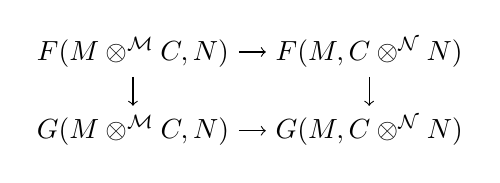
\begin{tikzpicture}
	\node (LT) at (0, 1) {$F(M \otimes^{\cM} C, N)$};
	\node (LB) at (0, 0) {$G(M \otimes^{\cM} C, N)$};
	\node (RT) at (3, 1) {$F(M, C \otimes^{\cN} N)$};
	\node (RB) at (3, 0) {$G(M, C \otimes^{\cN} N)$};
	\draw [->] (LT) -- node [left] {$$} (LB);
	\draw [->] (LT) -- node [above] {$$} (RT);
	\draw [->] (RT) -- node [right] {$$} (RB);
	\draw [->] (LB) -- node [below] {$$} (RB);
	%\node at (0.5, 1) {$\ulcorner$};
	%\node at (1.5, 0.5) {$\lrcorner$};
\end{tikzpicture}.
\end{center}
\end{definition}


\begin{definition}
	Let $\cA$ and $\cB$ be right and left $\cC$-module categories, respectively. The {\em Deligne tensor product $\cA \boxtimes_{\cC} \cB$} is the universal linear category admitting a $\cC$-balanced multilinear functor $\boxtimes_{\cC}: \cA \times \cB \to \cA \boxtimes_{\cC} \cB$. That is, there exists a $\cC$-balanced multilinear functor $\boxtimes_{\cC}: \cA \times \cB \to \cA \boxtimes_{\cC} \cB$ which induces, for all linear categories $\cD$, an equivalence between the categories of $\cC$-balanced multilinear functors $\cA \times \cB \to \cD$ and linear functors $\cA \boxtimes_{\cC} \cB \to \cD$. 
\end{definition}

If it exists, the Deligne tensor product is unique up to an equivalence, which in turn is unique up to unique natural isomorphism. Equivalently, the 2-category of linear categories representing the Deligne tensor product is either contractible or empty. 

\begin{theorem} \label{thm:DelignePrdtOverATCExists}
	Let $\cC$ be a finite tensor category and let $\cA_{\cC}$ and ${}_{\cC}\cB$ be finite right and left $\cC$-module categories, respectively. Then,
	\begin{enumerate}
		\item The Deligne tensor product $\cA \boxtimes_{\cC} \cB$ exists and is a finite linear category;
		\item If $\cA = \Mod{A}{}(\cC)$ and $\cB = \Mod{}{B}(\cC)$, then $\cA \boxtimes_{\cC} \cB \simeq \Mod{A }{B}(\cC)$;
	\end{enumerate} 
Moreover if $\cC$ is rigid, then 	
	\begin{enumerate}
		\item[(3)] The functor $\boxtimes_{\cC}$ is exact in each variable and satisfies 
		\begin{equation*}
			\hom_{\cA}(x,x') \otimes \hom_{\cB}(y, y') \cong \hom_{\cA \boxtimes_{\cC} \cB} (x \boxtimes_{\cC} y, x' \boxtimes_{\cC} y'),
		\end{equation*}
		\item[(4)] If $F: \cA \times \cB \to \cD$ is a $\cC$-balanced multilinear functor which is exact in each variable, then it defines an exact functor $\overline{F}: \cA \boxtimes_{\cC} \cB \to \cD$. 
	\end{enumerate} 
\end{theorem}

\begin{proof}
	When $\cC = \Vect_k$, this is classical [Deligne (Prop 5.13)] (see also [EGNO 1.46.2]).
	By Theorem \ref{thm:EGNO2.11.6} to show (1) and (2) it is enough to assume that $\cA = \Mod{A}{}(\cC)$ and $\cB = \Mod{}{B}(\cC)$ and show that $\Mod{A }{B}(\cC)$ has the desired universal property. Tensoring a left $A$-module and a right $B$-module gives a canonical $\cC$-balanced multilinear functor 
		\begin{equation*}
			T: \Mod{A}{}(\cC) \times \Mod{}{B}(\cC) \to \Mod{A}{B}(\cC),  
		\end{equation*}
and we will show that $T$ induces an equivalence between $\cC$-balanced multilinear functors $\cA \times \cB \to \cD$ and linear functors out of $\Mod{A}{B}(\cC)$.
	
	To this end, let $F:\Mod{}{A}(\cC) \times \Mod{B}{}(\cC) \to \cD$ be a $\cC$-balanced multilinear functor.  
	There is a unique right exact linear functor $\overline F: \Mod{B}{A}(\cC) \to \cA$ such that $F = \overline{F} \circ T$ which is defined as follows. On free bimodules $A \otimes X \otimes B \cong T(A \otimes X, B)$, we necessarily have $\overline{F}(A \otimes X \otimes B) \cong F(A \otimes X, B)$. Since  every $A$-$B$-bimodule $X$ is a coequalizer of free $A$-$B$-bimodules, namely the canonical coequalizer  
	\begin{equation*}
		X \leftarrow A \otimes X \otimes B \leftleftarrows A \otimes A \otimes X \otimes B \otimes B,
	\end{equation*}
	and since $\overline{F}$ is right exact the result follows.
	
	If $\cC$ is rigid, then by Lemma \ref{lma:RigidIsExact} the functor $T = \boxtimes_{\cC}$ is exact in each variable. The formula in (3) then follows as a standard exercise in using duals. Finally let $F: \cA \times \cB \to \cD$ be a $\cC$-balanced multilinear functor which is exact in each variable and let $\overline{F}: \cA \boxtimes_\cC \cB \to \cD$ be its linear extension (which is always right exact). Since $F$ is exact in each variable, $\overline{F}$ preserves left exact sequences of free $A$-$B$-bimodules (where the maps are also free). Since every $A$-$B$-bimodule has a functorial resolution by free $A$-$B$-bimodules (coming from the above mentioned coequalizer), a diagram chase shows that $\overline{F}$ is also left exact. Hence (4) is also satisfied. 
\end{proof}


%\begin{proposition}[]
%	Let $\cA$ and $\cB$ be finite linear categories. Then,
%	\begin{enumerate}
%		\item The Deligne tensor product $\cA \boxtimes \cB$ exists and is a finite linear category;
%		\item If $\cA = \Mod{A}{}$ and $\cB = \Mod{B}{}$, then $\cA \boxtimes \cB \simeq \Mod{A \otimes B}{}$;
%		\item The functor $\boxtimes$ is exact in each variable and satisfies 
%		\begin{equation*}
%			\hom_{\cA}(x,x') \otimes \hom_{\cB}(y, y') \cong \hom_{\cA \boxtimes \cB} (x \boxtimes y, x' \boxtimes y'),
%		\end{equation*}
%		\item If $F: \cA \times \cB \to \cC$ is a multilinear functor which is exact in each variable, then it defines an exact functor $\overline{F}: \cA \boxtimes \cB \to \cC$. 
%	\end{enumerate} 
%\end{proposition}


\begin{remark}
	We may use the case $\cC= \Vect_k$ to rewrite part the data  of a tensor category as a linear category $\cD$ equipped with an object $1 \in \cD$ and a linear functor $\otimes: \cD \boxtimes \cD \to \cD $, together with natural transformations $\alpha$, $\lambda$, and $\rho$, as before. 
\end{remark}

\begin{remark}
	If ${}_{\cD}\cA_{\cC}$ and ${}_{\cC}\cB_{\cE}$ are bimodule categories, then the actions of $\cD$ and $\cE$ induce a $\cD$-$\cE$-module category structure on $\cA \boxtimes_{\cC} \cB$. 
\end{remark}

\begin{lemma} \label{Lma:FunctorsAsATensorPdt}
	If $\cC$ is a finite tensor category and $\cM$ and $\cN$ are finite left $\cC$-module categories then the natural functor induces an equivalence
	\begin{equation*}
		\Fun_\cC(\cM, \cC) \boxtimes_\cC \cN \simeq \Fun_\cC(\cM,\cN).
	\end{equation*}
	Here $\Fun_\cC$ denotes the category of (right exact) $\cC$-module functors. 
	Moreover, if $\cM$ and $\cN$ are bimodule categories, then the above equivalence is a bimodule equivalence. 
\end{lemma}

\begin{proof}
	The last sentence follows since in that case the natural functor is a bimodule functor. By the Theorem \ref{thm:EGNO2.11.6}, there exist algebra objects $A, B \in \cC$ and equivalences $\cM \simeq \Mod{}{A}(\cC)$ and $\cN \simeq \Mod{}{B}(\cC)$. We show that both sides of the above equation are naturally equivalent to $\Mod{A}{B}(\cC)$, the category of $A$-$B$-bimodule objects in $\cC$. The equivalence $\Fun_\cC(\cM, \cN) \simeq \Mod{A}{B}(\cC)$ (\cite[Prop 2.12.2]{EGNO}) can be seen by mirroring the classical proof. A bimodule clearly gives rise to such a functor, and given a functor $f$, we obtain an $A$-$B$-bimodule $f(A)$. By $\cC$-linearity $f(X \otimes A) \cong X \otimes f(A)  \cong (X \otimes A) \otimes_A f(A) $ is determined on free $A$-modules. Since every object of $\cM$ may be written as a (canonical) coequalizer of free $A$-modules,
	\begin{equation*}
		M \leftarrow M \otimes A \leftleftarrows M \otimes A \otimes A
	\end{equation*} 
the functor $f$ is equivalent to the one determined by the bimodule $f(A)$. Thus the natural map  $\Mod{A}{B}(\cC) \to \Fun_\cC(\cM, \cN)$ is essentially surjective. The above argument also shows it is fully-faithful, so that $\Fun_\cC(\cM, \cN) \simeq \Mod{A}{B}(\cC)$, which in particular shows $\Fun_\cC(\cM, \cC) \simeq \Mod{}{A}(\cC)$. Now the result follows from Theorem \ref{thm:DelignePrdtOverATCExists}.
%Tensoring a left $A$-module and a right $B$-module gives a canonical $\cC$-balanced bilinear functor 
%\begin{equation*}
%	T: \Mod{A}{}(\cC) \times \Mod{}{B}(\cC) \to \Mod{A}{B}(\cC). 
%\end{equation*}
%To complete the proof we must show this induces an equivalence,
%\begin{equation*}
%	\Mod{}{A}(\cC) \boxtimes_\cC \Mod{B}{}(\cC) \simeq \Mod{B}{A}(\cC).
%\end{equation*}
%When $\cC = \Vect$, this is classical. More generally we must show that the right-hand-side has the desired universal property. For this purpose let $F:\Mod{}{A}(\cC) \times \Mod{B}{}(\cC) \to \cA$ be a $\cC$-balanced bilinear functor. There is a unique right exact linear functor $\overline F: \Mod{B}{A}(\cC) \to \cA$ such that $F = \overline{F} \circ T$ which is defined as follows. On free bimodules $A \otimes X \otimes B \cong T(A \otimes X, B)$, we necessarily have $\overline{F}(A \otimes X \otimes B) \cong F(A \otimes X, B)$. Since $\overline{F}$ is right exact and every $A$-$B$-bimodule is a coequalizer of free $A$-$B$-bimodules, the result follows. 	
\end{proof}




%\CD{[Fix the ground ring to be $\CC$?  Linear categories will mean linear over $\CC$?]}



\subsection{Exact Module Categories}

We will now specialize to the case that $\cC$ is a finite rigid tensor category. 

\begin{definition}
	Let $\cC$ be a finite rigid tensor category. A (left) $\cC$-module category $\cM$ will be called {\em exact} if for any object $M \in \cM$ and  projective object $P \in \cC$, the object $P \otimes M$ is projective in $\cM$. 
\end{definition}

\begin{example}
	If $\cC$ is semisimple (e.g. $\cC = \Vect$), then $\cM$ is an exact module category if and only if it is also semisimple.
\end{example}

\begin{example}
	$\cC$ is exact considered as a $\cC$-, $\cC^{mp}$-, or $\cC \otimes \cC^{mp}$-module category. 
\end{example}

The following omnibus theorem summarizes the key properties of exact module categories: 
\begin{theorem}[ENGO]
	Let $\cC$ be a finite rigid tensor category, and let $\cM$, $\cM'$, $\cM''$ be exact $\cC$-module categories, and $\cN$ an arbitrary $\cC$-module category. Then,
	\begin{enumerate}
		\item $\cM$ has enough projectives [EGNO lemma 2.7.1]
		\item Every projective object in $\cM$  is injective, and vice versa. [EGNO Cor 2.7.4]
		\item $\Fun_{\cC}(\cM, \cM')$ is finite [EGNO Prop 2.13.5]; In particular $\cM \simeq \Fun_{\cC}(\cC, \cM)$ is finite.
		\item Composition $\Fun_{\cC}(\cM, \cM') \times \Fun_{\cC}(\cM', \cM'') \to \Fuc_{\cC}(\cM, \cM'')$ is exact in each variable. [EGNO Lemma 2.13.2]		
		\item Every additive (not a priori right exact) module functor $F:\cM \to \cN$ is exact. Hence every functor $F \in \Fun_{\cC}(\cM, \cM')$ is exact, and has exact left and right adjoints. Moreover, it follows that   $\Fun_{\cC}(\cM,\cM)$ is again a finite rigid tensor category. 
	\end{enumerate}
\end{theorem}

\subsection{Multi-Fusion categories} \label{sec-tc-fusion}

\CD{CD continues to vote for using 'fusion' rather than 'multifusion'}

\begin{definition}
A \emph{fusion category} is a tensor category $\cC$ satisfying the following conditions:
\begin{enumerate}
\item For all objects $a, b \in \cC$, the vector space $\Hom(a,b)$ is finite dimensional.
\item The category $\cC$ is semisimple, with finitely many simple objects.
\item For every object $a \in \cC$, there exists an object $\ld{a} \in \cC$ that is a left dual for $a$ and there exists an object $\rd{a} \in \cC$ that is a right dual for $a$.
\end{enumerate}
\end{definition}

\begin{remark}
Here for brevity we use ``fusion category" to refer to what has elsewhere gone under the name ``multi-fusion category".
\end{remark}

\begin{proposition}
If $\cC$ is a fusion category, then there exist monoidal functors $\ld{(-)} : \cC \ra \cC^{\mop}$ and $\rd{(-)} : \cC \ra \cC^{\mop}$ whose values on any object $a \in \cC$ are respectively a left dual object $\ld{(a)}$ and a right dual object $\rd{(a)}$ for $a$.
\end{proposition} \CD{This proposition doesn't actually depend on fusion, right?  Should change the statement so that only what is needed (existence of duals) is assumed.}

\begin{proof}
Define the functor $\ld{(-)}$ on objects by picking for each object $a \in \cC$ a left dual object $\ld{a} \in \cC$.  Also pick a unit map $u: \ld{a} \; a \ra 1$ and a counit map $v: 1 \ra a \; \ld{a}$ giving $\ld{a}$ the structure of a left dual to $a$.  Define the functor $\ld{(-)}$ on a morphism $f: a \ra b$ by $\ld{(f)} := (u_b \cdot \id_{\ld{a}}) (\id_{\ld{b}} \cdot f \cdot \id_{\ld{a}}) (\id_{\ld{b}} \cdot v_a)$.  (This morphism $\ld{(f)}$ is called the \emph{mate} of $F$.)  Next we want to see that this functor is monoidal.  Observe that the morphisms $\ld{b} \; \ld{a} \; a \; b \xra{u_a} \ld{b} \; b \xra{u_b} 1$ and $1 \xra{v_a} a \; \ld{a} \xra{v_b} a \; b \; \ld{b} \; \ld{a}$ show that $(\ld{b} \; \ld{a})$ is a left dual to $(a b)$.  There is therefore a uniquely determined isomorphism from $(\ld{b} \; \ld{a})$ to $\ld{(a b)}$.  These isomorphisms provide the left dual functor with a monoidal structure.  The right dual functor is analogous.  % In principle, need to check naturality and hexagon for those isos.
\end{proof}
% This fact is asserted in Bruce's thesis; the functor part is mentioned in Selinger Eg 4.4.

\begin{remark}
The monoidal functor $\ld{(-)}: \cC \ra \cC^{\mop}$ is an equivalence of tensor categories; the inverse functor is $\rd{(-)}: \cC^{\mop} \ra \cC$.
\end{remark}

\begin{definition}
A fusion category $\cC$ is \emph{pivotal} if the double left dual functor $\ldd{(-)}: \cC \xra{\ld{(-)}} \cC^{\mop} \xra{\ld{(-)}} \cC$ is equivalent to the identity functor as a monoidal functor.
\end{definition}

In other words, a fusion category is pivotal if the left dual functor $\ld{(-)}: \cC \ra \cC^{\mop}$ and the right dual functor $\rd{(-)}: \cC \ra \cC^{\mop}$ are monoidally equivalent.





\section{The Symmetric Monoidal 3-Category of Tensor Categories}



%In this section we describe the symmetric monoidal 3-category of tensor categories. 
There are several potential theories of symmetric monoidal 3-category which one could select to describe the 3-category of tensor categories. We will employ the theory of iterated complete Segal spaces described by Clark Barwick, \CSP{Get reference. Possible a reference to Simpson's work too?} or more precisely the symmetric monoidal variant thereof. There are two special categories which play a fundamental role in this theory. These are the simplex category $\Delta$ and Segal's category $\Gamma$. We start with a review of $\Gamma$ and its role in describing symmetric monoidal structures. Then we review $\Delta$ and the most basic aspects (mostly definitional) of the theory of symmetric monoidal $(\infty,n)$-categories. Finally we present our construction of the symmetric monoidal $(\infty,3)$-category of tensor categories. 

\subsection{Symmetric monoidal structures via the category $\Gamma$}

\begin{definition}
	The category  $\Gamma$ has objects finite (unpointed, possibly empty) sets, and a morphism in $\Gamma$ from $A$ to $B$ consists of a function $f: A \to P(B)$, satisfying $f(x) \cap f(y) = \emptyset$ if $x \neq y$, where $P(B)$ denotes the power-set of $B$. 
\end{definition}

This category was introduced by Segal in \cite{Segal-Categories and Cohomology Theories}.  The opposite category $\Gamma^\textrm{op} \simeq Fin_*$ is the category of finite pointed sets. Let $(m) = \{ 1, 2, \dots, m\}$. For each element $a \in A$, there exists a canonical map $i_a: (1) \to A$, which is defined by setting $i_a(1) = \{a\} \subseteq A$. If $C$ is a category with finite products, then the category of commutative monoids in $C$ is equivalent to the category of functors $M:\Gamma^{op} \to C$ such that for all $A\in \Gamma$ the following {\em Segal map} is an isomorphism
\begin{equation*}
	\prod_{a \in A} i_a^*: M(A) \to \prod_{a \in A} M(1).
\end{equation*}
It will be instructive to spell this out explicitly. The case $A=\emptyset$ ensures that $M(\emptyset) = 1$, the terminal object of $C$. More generally $M(A) \cong M^{\times |A|}$. Maps in $\Gamma$ express ways to combine a $B$-tuple of elements of $M$ into an $A$-tuple of elements in $M$. Explicitly $f: A \to P(B)$
induces a map $f^*: M^{\times |B|} \to M^{\times |A|}$ which sends the $B$-tuple $(m_b)_{b \in B}$ to the $A$-tuple $(n_a)_{a \in A}$ where the element $n_a \in M$ is obtained by multiplying together all the elements $m_b$ where $b$ ranges over the elements in $f(a) \subseteq B$. This is a well-defined operation when $M$ is a commutative monoid, and conversely every such functor arises from a monoid in this manner. 

This generalizes to higher categories as well; the 2-category of symmetric monoidal categories is (weakly) equivalent to the 2-category of {\em strict} functors $\Gamma^{op} \to \Cat$ such that for each $A \in \Gamma$ the Segal maps are equivalences. Naively we expect this to mimic the case for monoids; a monoidal category $(M, \otimes)$ should give rise to a functor $\Gamma^\text{op} \to \Cat$ sending a set $A$ to $M^{\times |A|}$. However we immediately run into difficulty when we try to define functors for each map $f$ in $\Gamma$. Philosophically, we expect $f$ to induce a functor which sends a $B$-tuple of objects of $M$ to an $A$-tuple of objects of $M$ by multiplying together the objects of each $f(a)$-subtuple using the tensor product $\otimes$. However, unless $(M, \otimes)$ is a {\em strict} monoidal category, there is no canonical way to do this. We must choose an ordering and a bracketing of the elements indexed by each $f(a)$. Furthermore, even if we supply such choices, the result is not compatible with composition; we do not obtain a functor in this way. 

This leaves us with two possible avenues of pursuit:
\begin{enumerate}
	\item We relax our goal of obtaining a {\em strict} functor. The functors $f^*$ described above are not compatible with composition of maps in $\Gamma$, but they are compatible up to natural isomorphism of functor. In fact there are canonical coherent families of such natural isomorphisms and we obtain a {\em weak} functor from $\Gamma^\text{op}$ to the 2-category $\Cat$. 
	\item We realize that our initial guess that $A \mapsto M^{\times |A|}$ may have been overly optimistic. We content ourselves to have a strict functor $M: \Gamma^\text{op} \to \Cat$ where $M(A)$ is merely {\em equivalent} to  $M^{\times |A|}$. 
\end{enumerate}
Either of these options may be employed, and both give rise to equivalent ways to encode symmetric monoidal structures. The former option is only tenable if we have a tractable theory of weak functors at our disposal. For the case of symmetric monoidal categories we need a weak theory for 2-categories, and indeed there is a well established and usable theory. This option is entirely reasonable in that case. 

However in this paper we ultimately wish to describe a symmetric monoidal 3-category. Option (1) would generally require a robust theory of 4-categories and their weak functors. It is possible to do this using the theory of iterated complete Segal spaces, a model of $(\infty, n)$-categories which we will describe in the next section, but it is just as easy (and perhaps more explicit) to pursue the later option from the start. 

In the case where the monoidal structure in question is defined via a universal property, (which is the case of our primary interest) this second option has a particularly managable solution. Again, it is instructive to consider the 1-categorical case first. To this end we will now describe how the symmetric monoidal category of vector spaces may be encoded as a strict functor from $\Gamma^\text{op}$ to $\Cat$. 

The monoidal structure in $\Vect$ is given by the tensor product of vector spaces, which is defined by a well-known universal property. The tensor product of $V_1$ and $ V_2$ is a universal vector space receiving a bilinear map from $V_1 \times V_2$. In other words, the tensor product $V_{12}$ comes equipped with a bilinear map  $V_1 \times V_2 \to V_{12}$, inducing for all vector spaces $W$ a natural bijection between bilinear maps $V_1 \times V_2 \to W$ and linear maps $V_{12} \to W$. We will say that the bilinear map  $V_1 \times V_2 \to V_{12}$ {\em realizes $V_{12}$ as a tensor product}. As with all universal properties, if the tensor product exists then it is unique up to unique isomorphism, and so it is common practice to write $V_{12} = V_1 \otimes V_2$ for any choice of tensor product.

To define $\otimes$ as an honest functor, though, we must choose a specific representative for each pair $V_1$ and $V_2$. The standard method is to {\em define} the vector space $V_1 \otimes V_2$ as the vector space of linear combinations of formal expressions $v_1 \otimes v_2$ with $v_i \in V_i$, modulo the obvious relations. This operation is not strictly associative (for example the underlying sets of $(V_1 \otimes V_2) \otimes V_3$ and $V_1 \otimes (V_2 \otimes V_3)$ are distinct), but the universal property ensures it is associative up to canonical coherent natural isomorphism.

We will now describe how to encode this symmetric monoidal structure as a strict functor,
\begin{equation*}
	\Vect: \Gamma^\text{op} \to \Cat.
\end{equation*}  
In our initial naive attempt at constructing such a functor we identified the key difficulty: given a $B$-tuple of vector spaces, and a map $f: A \to P(B)$ in $\Gamma$ (i.e. a certain collection of subsets $f(a) \subseteq B$) we need to choose a way to take the tensor product of each of the corresponding subtuples. Rather then make such a choice for each $f$ (which yields only a weak functor $\Gamma^\text{op} \to \Cat$) we will enlarge $\Vect^{\times |B|}$ to include choices of these tensor products for each subset of $B$. 

The most canonical way to do this is to define $\Vect(B)$ to include all possible representatives of the tensor product for each of the subsets of $B$. Thus we obtain the following definition of the category $\Vect(B)$: 
\begin{itemize}
	\item The objects consist of a pair of collections, one of vector spaces $\{ V_S \}$ indexed by the subsets $S \subseteq B$, 
	the other of bilinear maps $ \{ v_{S,S'}: V_S \times V_{S'} \to V_{S \cup S'} \} $ 
	indexed by pairs of disjoint subsets $S, S' \subseteq B$. These are required to satisfy the following conditions:
	\begin{enumerate}
		\item $V_{\emptyset} = k$; 
		\item $v_{S,S'}$ realizes $V_{S \cup S'}$ as the tensor product of $V_S$ and $V_{S'}$;
		\item If $S, S', S'' \subseteq B$ are three pairwise disjoint subsets, then the following square of multilinear maps commutes:
	\begin{center}
	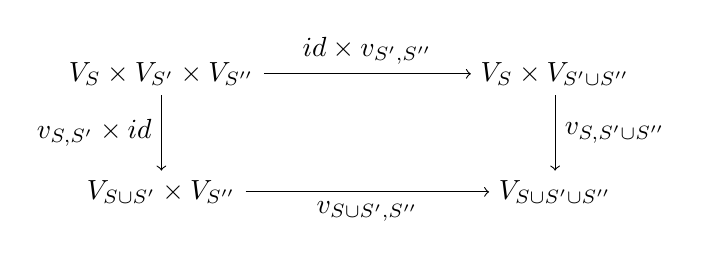
\begin{tikzpicture}
		\node (LT) at (0, 1.5) {$V_S \times V_{S'} \times V_{S''}$};
		\node (LB) at (0, 0) {$V_{S \cup S'} \times V_{S''}$};
		\node (RT) at (5, 1.5) {$V_S \times V_{S' \cup S''}$};
		\node (RB) at (5, 0) {$V_{S \cup S' \cup S''}$};
		\draw [->] (LT) -- node [left] {$v_{S,S'} \times id$} (LB);
		\draw [->] (LT) -- node [above] {$id \times v_{S', S''}$} (RT);
		\draw [->] (RT) -- node [right] {$v_{S, S' \cup S''}$} (RB);
		\draw [->] (LB) -- node [below] {$v_{S \cup S', S''}$} (RB);
		%\node at (0.5, 1) {$\ulcorner$};
		%\node at (1.5, 0.5) {$\lrcorner$};
	\end{tikzpicture}
	\end{center}
	\end{enumerate} 
	\item The morphisms from $\{ V_S, v_{S, S'} \} \to \{ W_S, w_{S, S'} \}$ consist of collections of linear maps $\{ \phi_S: V_S \to W_S \}$, such that $\phi_{\emptyset} = id$ and for each pair of disjoint subsets $S, S' \subseteq B$ the following square commutes:
	\begin{center}
	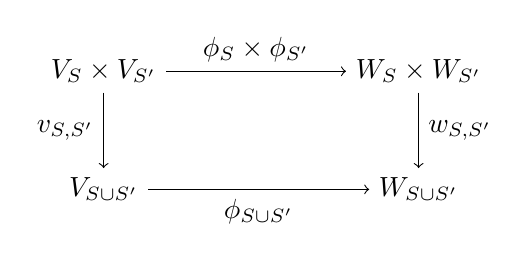
\begin{tikzpicture}
		\node (LT) at (0, 1.5) {$V_S \times V_{S'}$};
		\node (LB) at (0, 0) {$V_{S \cup S'}$};
		\node (RT) at (4, 1.5) {$W_S \times W_{S'}$};
		\node (RB) at (4, 0) {$ W_{S \cup S'}$};
		\draw [->] (LT) -- node [left] {$v_{S,S'}$} (LB);
		\draw [->] (LT) -- node [above] {$\phi_S \times \phi_{S'}$} (RT);
		\draw [->] (RT) -- node [right] {$w_{S,S'}$} (RB);
		\draw [->] (LB) -- node [below] {$\phi_{S \cup S'}$} (RB);
		%\node at (0.5, 1) {$\ulcorner$};
		%\node at (1.5, 0.5) {$\lrcorner$};
	\end{tikzpicture}.
	\end{center}
\end{itemize}
Thus an object of $\Vect(A)$ consist partly of an $A$-tuple of vector spaces, namely $ (V_{\{a\}})_{a \in A}$. Each vector space $V_S$ should then be thought of as a {\em choice} of simultaneous tensor product of all the $V_{\{a\}}$ where $a \in S$. The data and conditions of an object of $\Vect(A)$ make this philosophical viewpoint precise, and similarly for the morphisms of $\Vect(A)$. 

The assignment $A \mapsto \Vect(A)$ gives a functor $\Vect: \Gamma^{op} \to \Cat$, for if $f: A \to P(B)$, then we obtain a functor $f^*: \Vect(B) \to \Vect(A)$ as follows. If $T \subseteq A$, let $f(T) = \cup_{a \in T} f(a) \subseteq B$. Then an object $\{ V_S, v_{S,S'} \}_{S, S' \subseteq B}$ of $\Vect(B)$ is sent via $f^*$ to the object $\{ W_T, w_{T, T'} \}_{T, T' \subseteq A} \in \Vect(A)$, where 
\begin{equation*}
	W_T = V_{f(T)} \quad \textrm{and} \quad  w_{T, T'} = v_{f(T), f(T')}.
\end{equation*}
This is easily seen to be strictly compatible with composition in $\Gamma^\text{op}$. Moreover, since the tensor product is defined by a universal property, the forgetful functor $\Vect(A) \to \Vect^{\times |A|}$ is an equivalence of categories, as desired.  


\subsection{Symmetric Monoidal $(\infty,3)$-Categories}

\begin{definition}
	The simplex category $\Delta$ is a skeleton of the category of finite non-empty totally ordered sets and order preserving maps. The objects of $\Delta$ are the ordered sets $[n] = \{ 0 < 1 < 2 < \cdots < n\}$. A {\em $k$-simplex} of $[n]$ is a strictly order preserving map $[k] \to [n]$. There are $ {n+1}\choose {k+1}$ such maps. $0$-simplices will be called {\em vertices} and $1$-simplices will be called {\em edges}. 
\end{definition}

This is the category of combinatorial simplices. The vertices of $[n]$ have a natural ordering induced from the ordering of $[n]$. Let $[m + n]$ denote the ordered concatenation of $[m]$ with $[n]$. We thus obtain the following commuting square,
\begin{equation} \label{Eqn:Segal-Co-Map}
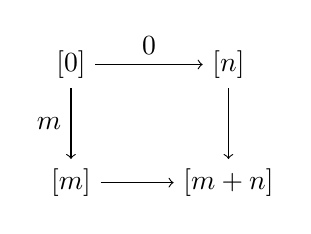
\begin{tikzpicture}[baseline = 0.75cm]
	\node (LT) at (0, 1.5) {$[0]$};
	\node (LB) at (0, 0) {$[m]$};
	\node (RT) at (2, 1.5) {$[n]$};
	\node (RB) at (2, 0) {$[m+n]$};
	\draw [->] (LT) -- node [left] {$m$} (LB);
	\draw [->] (LT) -- node [above] {$0$} (RT);
	\draw [->] (RT) -- node [right] {$$} (RB);
	\draw [->] (LB) -- node [below] {$$} (RB);
	%\node at (0.5, 1) {$\ulcorner$};
	%\node at (1.5, 0.5) {$\lrcorner$};
\end{tikzpicture}
\end{equation}
where $0: [0] \to [n]$ and $m: [0] \to [m]$ denote the first and last vertices, respectively. 


Let $C$ be a category. The category of {\em simplcial objects of $C$} is the functor category $Fun(\Delta^\textrm{op}, C) = sC$. We write $X_\bullet$ for such a functor, and let $X_n$ denote the value assigned $[n] \in \Delta$. A {\em category internal to $C$} is a simplicial object $X$, such that the diagrams induced by those in equation (\ref{Eqn:Segal-Co-Map}),
\begin{center}
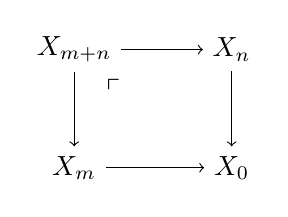
\begin{tikzpicture}
	\node (LT) at (0, 1.5) {$X_{m+n}$};
	\node (LB) at (0, 0) {$X_m$};
	\node (RT) at (2, 1.5) {$X_n$};
	\node (RB) at (2, 0) {$X_0$};
	\draw [->] (LT) -- node [left] {$$} (LB);
	\draw [->] (LT) -- node [above] {$$} (RT);
	\draw [->] (RT) -- node [right] {$$} (RB);
	\draw [->] (LB) -- node [below] {$$} (RB);
	\node at (0.5, 1) {$\ulcorner$};
	%\node at (1.5, 0.5) {$\lrcorner$};
\end{tikzpicture}
\end{center}
are a pullback diagrams. For a general simplicial object $X$, these commuting squares will be called {\em Segal squares} and if they are pullback squares we will say that $X$ satisfies the {\em Segal condition}. Hence a category internal to $C$ is a simplicial object satisfying the Segal condition. 

This may be contrasted with the notion of a category enriched to $C$, which consists of a {\em set} of objects together with hom objects $Hom(x,y) \in C$ (as opposed to an object $X_0 \in C$ of objects). Under certain conditions these notions may be related. Recall that a category is {\em extensive} (or {\em infinitary extensive}) if it admits small coproducts and coproducts are disjoint and stable under pullback. If $C$ is an extensive category with a terminal object, then a category enriched in $C$ is merely an internal category $X$ in which the object $X_0$ is {\em discrete}, i.e. a coproduct of terminal objects. Examples of extensive categories with terminal objects include the categories of sets, any category of presheaves (or more generally any Grothendieck topos), the category of topological spaces, and the category of small categories. 

\begin{example}
	An ordinary (small) category is a category enriched in sets.
\end{example}

Thus a category $C$ may equivalently be regarded as simplical set $NC_\bullet$ called the {\em nerve of $C$}. The $n^\textrm{th}$ set of $NC_{\bullet}$ is given by the formula
\begin{equation*}
	NC_n := \sqcup_{x_0, x_1, \dots, x_n \in C_0} \hom_C(x_0, x_1) \times \hom_C(x_1, x_2) \times \cdots \times \hom_C(x_{n-1}, x_n).
\end{equation*}
Regarding the ordered set $[n] \in \Delta$ as a category, $NC_n$ may be viewed as the set of functors from $[n]$ to $C$. 

\begin{example}
	A {\em strict 2-category} is a category enriched in categories.
\end{example}

Thus a strict 2-category may equivalently be regarded as a simplical object with values in $\Cat$, such that $X_0$ is a set (thought of as a discrete category), and such the the Segal squares are pullback squares. Since $X_0$ is a set, these pullbacks may be simultaneously regarded as pullbacks in the 1-category of categories and functors or as weak (or homotopy) pullbacks in the 2-category of categories, functors, and natural transformations. If $X_0$ is allowed to be a general category, these two notions of pullback may differ. 

\begin{definition}
	Let $\sSet$ denote the category of simplicial sets. An {\em $n$-fold simplicial space} is a functor $X: (\Delta^\textrm{op})^{\times n} \to \sSet$. A {\em $\Gamma$-$n$-fold simplicial space} is a functor $X: \Gamma^\textrm{op} \times (\Delta^\textrm{op})^{\times n} \to \sSet$.
\end{definition}

The categories of $n$-fold simplicial spaces and $\Gamma$-$n$-fold simplicial spaces admit combinatorial model structures which give robust theories of $(\infty, n)$-categories and symmetric monoidal $(\infty, n)$-categories, respectively. This is the context in which the cobordism hypothesis has been proven and is the context in which we frame our results. The fibrant objects of these model categories are the so-called $n$-fold complete Segal spaces and symmetric monoidal $n$-fold complete Segal spaces, respectively (these later are sometimes called special $\Gamma$-$n$-fold complete Segal spaces).
These fibrant objects enjoy many desirable properties. For example, the weak equivalences between fibrant objects are precisely the levelwise weak equivalences. Also many related constructions, like the homotopy category of an $(\infty, n)$-category, have simple direct descriptions for these fibrant objects. 

On the other hand, many examples occurring { in nature} do not arise as $n$-fold complete Segal spaces or as symmetric monoidal $n$-fold complete Segal spaces. For example in \cite{Lurie}, the $(\infty, n)$-category of cobordisms is constructed as a $n$-fold Segal space which is {\em not} complete. There are a number of classes of $n$-fold simplicial spaces which are intermediary between general $n$-fold simplicial spaces and the fibrant $n$-fold complete Segal spaces. For many purposes these intermediary objects are just as good as their fibrant replacement. One such intermediate notion is that of $n$-fold Segal category, and it is this intermediate notion to which we now turn. 
%\begin{definition}
%	An $n$-fold simplicial space $X$ is {\em essentially constant} if, when regarded as a functor $X: (\Delta^\textrm{op})^{\times n} \to h\textrm{-}(sSet)$, it is equivalent to a constant functor, where $h\textrm{-}(sSet)$ denotes the homotopy category of simplicial sets.  
%\end{definition}
%
We may regard any $n$-fold simplicial space as a simplicial object in $(n-1)$-fold simplicial spaces. A $0$-fold simplicial space is understood to be a simplicial set. 

\begin{definition}
	A $0$-fold simplicial space (i.e. a simplicial set) is a {\em $0$-fold Segal category} if it is a Kan complex. An $n$-fold simplicial space $X$, regarded as a simplicial object $X_\bullet$ in $(n-1)$-fold simplicial spaces is an {\em $n$-fold Segal category} if the following conditions are satisfied
		\begin{enumerate}
			\item The $(n-1)$-fold simplicial space $X_0$ is constant and discrete.
			\item Each of the $(n-1)$-fold simplicial spaces $X_k$ is an $(n-1)$-fold Segal category.
			\item For every $m, k$, the Segal square,
			\begin{center}
			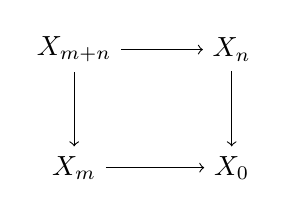
\begin{tikzpicture}
				\node (LT) at (0, 1.5) {$X_{m+n}$};
				\node (LB) at (0, 0) {$X_m$};
				\node (RT) at (2, 1.5) {$X_n$};
				\node (RB) at (2, 0) {$X_0$};
				\draw [->] (LT) -- node [left] {$$} (LB);
				\draw [->] (LT) -- node [above] {$$} (RT);
				\draw [->] (RT) -- node [right] {$$} (RB);
				\draw [->] (LB) -- node [below] {$$} (RB);
				%\node at (0.5, 1) {$\ulcorner$};
				%\node at (1.5, 0.5) {$\lrcorner$};
			\end{tikzpicture}
			\end{center}
			is a homotopy pull-back square of $(n-1)$-fold simplical spaces, computed with the $(\infty, n-1)$-model structure.
		\end{enumerate}
	\end{definition}
This final condition requires some explanation. The Segal square must realize $X_{m+n}$ as the homotopy fiber product $X_m \times_{X_0}^h X_n$, and this homotopy fiber product must be computed in the $(\infty, n-1)$-category model structure on $(n-1)$-fold simplicial sets. Moreover $X_{m+n}$ may not be levelwise equivalent to this homotopy fiber product, but merely weakly equivalent in this model structure. Fortunately, we require that $X_0$ is a discrete $(n-1)$-fold simplcial space. In this case the homotopy fiber product simplifies and is merely the ordinary fiber product. Thus condition (3) is equivalent to:

\begin{enumerate}
	\item [(3')] For every $m$ and $k$ the Segal map $X_{m+n} \to X_m \times_{X_0} X_n$ is an equivalence of $(n-1)$-fold Segal categories. 
\end{enumerate}

Moreover equivalences between $n$-fold Segal categories admit a fairly tractable inductive recognition principle. To describe this me must introduce a few auxiliary concepts. Let $X$ be an $n$-fold Segal category. Recall that $X_0$ is a constant discrete simplicial space, and so may be regarded as a set. We call the elements of $X_0$ objects of $X$. 
Inductively we will define three functorial constructions:
\begin{itemize}
	\item For every pair of objects $a,b \in X_0$, an $(n-1)$-fold Segal category $Hom_X(a,b)$.
	\item A category $\mathit{h}X$, called the {\em homotopy category} of $X$.
	\item A set $\pi_0 X$, which is the set of isomorphism classes of objects of $\mathit{h}X$. 
\end{itemize}
Once we have these constructions, equivalences of $n$-fold Segal categories are easily recognized: they are precisely those maps $f:X \to Y$ of $n$-fold simplicial spaces which induce bijections $\pi_0 f: \pi_0 X \to \pi_0 Y$, 
% equivalences of homotopy categories $\mathit{h}f:\mathit{h}X \to \mathit{h}Y$ 
and which induce equivalences of $(n-1)$-fold Segal categories $Hom_X(a,b) \to Hom_Y(fa, fb)$ for every pair of objects $a,b \in X_0$. Such maps also induce equivalences $\mathit{h}f:\mathit{h}X \to \mathit{h}Y$.

Given a pair objects $a,b \in X_0$ in an $n$-fold Segal category $X$, the $(n-1)$-fold Segal category $Hom_X(a,b)$ is defined to be the fiber over $(a,b) \in X_0 \times X_0$ of the map $(d_0, d_1): X_1 \to X_0 \times X_0$.  
\begin{center}
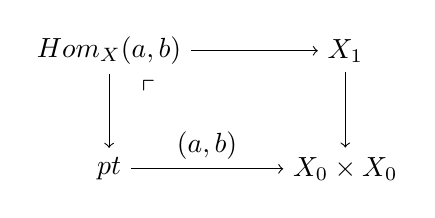
\begin{tikzpicture}
	\node (LT) at (0, 1.5) {$Hom_X(a,b)$};
	\node (LB) at (0, 0) {$pt$};
	\node (RT) at (3, 1.5) {$X_1$};
	\node (RB) at (3, 0) {$X_0\times X_0$};
	\draw [->] (LT) -- node [left] {$$} (LB);
	\draw [->] (LT) -- node [above] {$$} (RT);
	\draw [->] (RT) -- node [right] {$$} (RB);
	\draw [->] (LB) -- node [above] {$(a,b)$} (RB);
	\node at (0.5, 1) {$\ulcorner$};
	%\node at (1.5, 0.5) {$\lrcorner$};
\end{tikzpicture}
\end{center}
The homotopy category $\mathit{h}X$ has the same object set $X_0$, and the morphisms set between two objects is given as the set $Hom_{\mathit{h}X}(a,b) := \pi_0 Hom_X(a,b)$. For every triple of objects $a,b,c \in X_0$ we have a similar $(n-1)$-fold Segal category $Hom_X(a,b,c)$ which is defined as the fiber in $X_2$ over the point $(a,b,c)$ in $X_0 \times X_0 \times X_0$. Since $X$ is an $n$-fold Segal category we have induced maps of $(n-1)$-fold Segal categories,
\begin{equation*}
	Hom_X(a,b) \times Hom_X(b,c) \stackrel{\simeq}{\longleftarrow} Hom_X(a,b,c) \stackrel{}{\longrightarrow} Hom_X(a,c).
\end{equation*}
Composition in $\mathit{h}X$ is given by the induced map of sets,
\begin{equation*}
	 Hom_{\mathit{h}X}(a,b) \times Hom_{\mathit{h}X}(b,c) \cong \pi_0 Hom_X(a,b,c)\to \pi_0 Hom_X(a,c) = Hom_{\mathit{h}X}(a,c).
\end{equation*}

\begin{example}
	If we regard a set as a constant simplicial space, then the nerve of a category $NC$ is a 1-fold Segal category. $NC_0 = \textrm{ob}\ C$ and the space $Hom_{NC}(a,b)$ are the sets $Hom_C(a,b)$. Moreover $hNC \cong C$ is isomorphic to the category $C$. 
\end{example}

\begin{example}
	A strict 2-category $C$ may be regarded as a simplical object $C_\bullet$ in $\Cat$ whose $n^\textrm{th}$ category is given by the usual formula
	\begin{equation*}
		C_n := \sqcup_{x_0, x_1, \dots, x_n \in C_0} \hom_C(x_0, x_1) \times \hom_C(x_1, x_2) \times \cdots \times \hom_C(x_{n-1}, x_n).
	\end{equation*}
	We obtain a 2-fold simplicial set by applying the nerve construction to each of these categories, which, by viewing a set as a discrete simplicial space, we regard as a 2-fold simplcial space $NC_{\bullet \bullet}$. Since $C_\bullet$ satisfies the Segal condition, one deduces that $NC_{\bullet \bullet}$ is a 2-fold Segal category. 
	\footnote{Alternatively, one may start with the simplicial category $C_\bullet$, as before and apply the {\em complete Segal space nerve} to each of the categories $C_n$. The $k^\text{th}$ space of this simplicial space $N^{CSS}_\bullet C_n$ is obtained by first constructing the functor category $Fun([k], C_n)$, then throwing away the non-invertible natural transformations, and finally applying the classifying space functor to the resulting groupoid. This alternative has the advantage that it produces a {\em complete} Segal space $N^{CSS} C_n$. However for our purposes these are equivalent constructions as the canonical map $N C_n \to N^{CSS} C_n$ is a weak equivalence in the complete Segal space model structure. 
	%[Cite the Joyal Teinery paper for the Quillen equivalence between Segal spaces and Quasi-categories]
	} We call the association $C \mapsto NC_{\bullet \bullet}$ the {\em 2-categorical nerve}. 
	\CSP{We should get a reference for this.}
\end{example}

\begin{lemma} \label{lma:2catnervereflectsequiv}
	A strict functor of strict 2-categories $F: C \to D$ is a weak equivalence if and only if the induced map of 2-fold Segal categories $NC_{\bullet \bullet} \to ND_{\bullet \bullet}$ is an equivalence. 
\end{lemma}

\begin{proof}
	The functor $F$ is a weak equivalence if and only if 
	\begin{enumerate}
		\item it is essentially surjective on object, and
		\item for every pair of objects $a,b \in C$,  it induces an equivalence of categories $C(a,b) \to D(Fa, Fb)$.
	\end{enumerate}
On the other hand, a map of 2-fold Segal spaces $X \to Y$ is an equivalence if and only if
\begin{enumerate}
	\item it induces a bijection $\pi_0X \to \pi_0Y$, and
	\item for every pair of objects $a,b \in X_0$, it induces equivalences of 1-fold Segal spaces $Hom_X(a,b) \to Hom_Y(Fa, Fb)$.
\end{enumerate}
When $X = NC_{\bullet \bullet}$  is a 2-categorical nerve, $Hom_X(a,b) \cong NC(a,b)_{\bullet}$, so the second conditions are equivalent. Moreover, $\pi_0 NC_{\bullet \bullet}$ is easily seen to be the collection of equivalence classes of objects of $C$. Thus a functor inducing an equivalence of 2-categorical nerves induces a bijection on equivalence classes of objects. In particular if $F$ induces an equivalence of 2-categorical nerves, it is essentially surjective, and hence a weak equivalence of categories. It remains to see that a weak equivalence of categories necessarily induces a bijection on sets of equivalence classes of object. This follows as a well-known exercise.
\end{proof}

%If the $n$-fold Segal spaces $X_k$ are fibrant, that is complete, then these problems disappear. Weak equivalences between fibrant objects are computed levelwise, as are homotopy fiber products. 

%Thus in general we are left with the embarrassing responsibility of computing the correct homotopy fiber product $X_m \times_{X_0}^h X_n$, and showing that the canonical map from $X_{m+n}$ is a weak equivalence of $(\infty, n-1)$-categories. Fortunately there is another subclass of $n$-fold Segal spaces for which these two operations are relatively easy to perform: The {\em $n$-fold Segal categories}.

\begin{definition}
%   A $0$-fold Segal category is a Kan complex. An {\em $n$-fold Segal category} is an $n$-fold Segal space which satisfies
%   \begin{enumerate}
%   	\item $X_0$ is discrete, and
%   	\item for each $n$, $X_n$ is an $(n-1)$-fold Segal category. 
%   \end{enumerate}
	A {\em symmetric monoidal $n$-fold Segal category} (a.k.a. {\em special $\Gamma$-$n$-fold Segal category}) is a $\Gamma$-$n$-fold simplicial space $X$, which we view as a functor from $\Gamma^\textrm{op}$ to $n$-fold simplcial spaces, such that the following conditions are satisfied. 
	\begin{enumerate}
		\item $X_A$ is an $n$-fold Segal category for each $A \in \Gamma$. 
		\item For each set $A \in \Gamma$ (possibly empty) the canonical map,
		\begin{equation*}
			\prod_{a \in A} i_a^*: X_A \to \prod_{a \in A} X_{(1)}
		\end{equation*}
		is an equivalence of $n$-fold Segal categories. %\CSP{Should we also add the $X_{(0)} = pt$? We get $X_{(0)} \simeq pt$ for free.}
	%	\item (optional) The previous axiom implies that $X_\emptyset \simeq pt$. We assert that $X_\emptyset = pt$. 
	\end{enumerate}
\end{definition}

In the next section we will construct an example: $\TC$ the symmetric monoidal 3-fold Segal category of tensor categories. 

%Thus the goal of this section is to describe $\TC$ as a functor $\Gamma^{\op} \times (\Delta^{\op})^{\times 3} \to \sSet$. This is done in two stages. First we construct a nerve functor from the category of strict 2-categories to 2-fold Segal categories. This reduces the construction of $\TC$ to constructing a functor (also denoted $\TC$) from $\Gamma^{\op} \times \Delta^{\op}$ to the category of strict 2-categories and strict functors. As a warm-up, we first describe a functor $\lincat$ from $\Gamma^{\op}$ to strict 2-categories which serves as a model for the symmetric monoidal 2-category of linear categories. The functor $\TC$ is a more elaborate variation on this construction. 

%We now describe how a strict 2-category gives rise to a 2-fold Segal category. This can be regarded as a 2-categorical nerve. %Later we will construct explicitly $\TC$ as a simplicial object in the category of strict 2-categories. Applying the previous 2-categorical nerve yields a 3-fold simplcial space which is shown to be a 3-fold Segal category. A variation on these constructions yields the $\Gamma$-3-fold Segal space $\TC$. 
%\begin{definition}
%	A strict 2-category is a category object $(C_1 \rightrightarrows C_0)$ in categories such that the category of objects $C_0$ is discrete (i.e. its only morphisms are identities). 
%\end{definition}
%A strict 2-category gives rise to a simplicial category 




\subsection{The symmetric monoidal 3-category of tensor categories} \label{sec-tc-threecat}


We now describe the symmetric monoidal 3-fold Segal category $\TC$. We first construct it as a functor from $(\Gamma \times \Delta)^\textrm{op}$ to strict 2-categories, such that the Segal maps are weak equivalences. We may obtain a $\Gamma$-3-fold simplicial spaces by applying the 2-categorical nerve levelwise. Lemma \ref{lma:2catnervereflectsequiv} implies that the result is indeed a symmetric monoidal 3-fold Segal category. 

Let $A$ be a finite set and $[n]\in \Delta$. The strict 2-category $\TC(A,n)$ will have objects which consist of collections of several tensor categories, bimodule categories, functors, and natural transformations which are required to satisfy a host of conditions. The 1- and 2-morphisms of $\TC(A,n)$ will be defined similarly. Morally, one should regard $\TC(A,n)$ as the 2-category consisting of $A$-tuples of length $n$ strings of composable bimodule categories. In other words, if one had a pre-existing notion of 3-category, then $\TC(A,n)$ should be thought of as functors from the category $A \times [n]$ into the weak 3-category $\TC$. 

The problem with implementing this straightforward idea is that one almost invariably fails to produce a functor from $(\Gamma \times \Delta)^\textrm{op}$ to a category. This is largely due to the fact that  composition of bimodule categories is only weakly defined. It is defined up to equivalence of bimdule categories which are in turn defined up to unique natural isomorphism, but this is not sufficient to obtain a {\em strict} functor on $(\Gamma \times \Delta)^\textrm{op}$. One solution is to enlarge $\TC(A,n)$ to include choices of all the possible composites that one would need in order to obtain a strict functor to strict 2-categories. The resulting $\TC(A,n)$ is what we now describe.

As we mentioned, the objects of $\TC(A,n)$ are certain collections of tensor categories, bimodule categories, and their various maps. These collections are parametrized by the $k$-faces of $[n]$ and collections of disjoint subsets of $A$. We summarize the data of an object $X \in \TC(A,n)$ in Tables \ref{Table:ObjectOfTC} and \ref{Table:ObjectOfTC2}.
\begin{table}[ht]
	\caption{Data and Conditions for an object of $\TC(A,n)$.}
	\begin{tabular}{c |ccccc}
	 subsets \textbackslash\ faces & vertex $i$ & edge $ij$ & 2-face $ijk$ & 3-face $ijk\ell$ & 4-face \\
	\hline
	$S$ 				& $X_{S;i}$ & $X_{S; ij}$ & $b_{S; ijk}$  & $\alpha_{S;ijk\ell}$ & (TCO3) \\
	$S, S'$ 			& $x_{S, S';i}$ & $x_{S, S';ij}$ & $\psi_{S, S'; i j k}$ & (TCO4) & \\
	$S, S', S''$ 		& $\alpha_{S, S', S'';i}$ & $\alpha_{S, S', S'';ij}$ & (TCO5) &  & \\
	\hline
	$S, S', S'', S''' $	& \multicolumn{2}{c}{ \tikz[baseline=-0.1cm]{\draw [->] (0,0) -| (-0.2, 0.15);} (TCO6) \tikz[baseline=-0.1cm]{\draw [->] (0,0) -| (0.2, 0.15);}}  &  &  & \\
	\end{tabular}
	\label{Table:ObjectOfTC}
\end{table}	
\begin{table}[ht]
	\caption{Description of the Data of an object of $\TC(A,n)$.}	
	\begin{tabular}{l p{11cm}}
		datum & description of datum \\ \hline
		$X_{S;i}$ & A tensor category \\
		$X_{S;ij}$ & An $X_{S;i}$-$X_{S,j}$-bimodule category. \\
		$b_{S; ijk}$ & An $X_{S;j}$-balanced $X_{S;i}$-$X_{S,k}$-bilinear functor from $X_{S;ij}\times X_{S;jk}$ to $X_{S;ik}$. \\
		$\alpha_{S;ijk \ell}$  & A natural isomorphism of $X_{S;j}$/$X_{S;k}$-balanced $X_{S'i}$-$X_{S;\ell}$-bimodule functors from $b_{S;i k \ell} \circ (b_{S;ijk} \times id_{X_{S;k\ell}})$ to $b_{S;ij \ell} \circ (id_{X_{S;ij}} \times b_{S;jk\ell})$. \\ \hline
		$x_{S, S';i}$ & A bilinear tensor functor from $X_{S;i} \times X_{S';i}$ to $X_{S \cup S'; i}$. \\
		$x_{S, S';ij}$ & A bilinear bimodule functor from $X_{S;ij} \times X_{S';ij}$ to $X_{S \cup S'; ij}$. \\
		$\psi_{S, S'; i j k}$ & A natural isomorphism of $X_{S;j} / X_{S';j}$-balanced bimodule functors from $x_{S,S'; ik} \circ (b_{S; ijk} \times b_{S';ijk})$ to $b_{S \cup S'; ijk} \circ (x_{S,S';ij} \times x_{S \cup S'; jk}) \circ  \tau $, where $\tau$ exchanges the middle two factors.  \\ \hline
		$\alpha_{S, S', S'';i}$ & A natural isomorphism of multilinear tensor functors from
		$x_{S \sqcup S', S'';i}\circ (x_{S,S';i} \times 1)$  to 
		$x_{S, S' \sqcup S'';i} \circ (1 \times x_{S', S'';i})$. \\
		$\alpha_{S, S', S'';ij}$ & A natural isomorphism of multilinear bimodule functors from
		$x_{S \sqcup S', S'';ij}\circ (x_{S,S';ij} \times 1)$  to 
		$x_{S, S' \sqcup S'';ij} \circ (1 \times x_{S', S'';ij})$. \\
	\end{tabular}
	\label{Table:ObjectOfTC2}
\end{table}
This data is required to satisfy a the following conditions: \\
\newcounter{itemcounter}
\begin{list}{(TCO\arabic{itemcounter})}{\usecounter{itemcounter}}
%	\setlength{\leftmargin}{0pt}
	\item  The functors $x_{S,S';i}$, $x_{S,S'; ij}$, and $b_{S;ijk}$ realize equivalences with the following Deligne tensor products:
	\begin{align*}
		X_{S \cup S'; i} &\cong X_{S; i} \boxtimes X_{S';i} \\ 
		X_{S \cup S'; ij} &\cong X_{S; ij} \boxtimes X_{S';ij} \\ 
		X_{S; ik} & \cong X_{S;ij} \boxtimes_{X_{S;j}} X_{S;jk}
	\end{align*}
	\item  $X_{\emptyset; i} \cong \Vect$, with $X_{\emptyset; ij}$, $b_{\emptyset; ijk}$, and $\alpha_{\emptyset; ijk\ell}$ the evident identity morphisms and bimodule category. Moreover when either $S$ or $S'$ equals $\emptyset$, the functors $x_{S,S'; i}$ and $x_{S, S'; ij}$ and the transformation $\psi_{S,S'; ijk}$ are the canonical ones.  
	\item  For every 4-simplex $ijk\ell m$, $\alpha_{S; -}$ satisfies the evident pentagon equation.

	\item  For every pair of disjoint subsets $S, S'$ and every 3-simplex $ijk\ell$, the `hexagon' equation in Figure \ref{fig:EqnSSijkObject} is satisfied. 
\begin{figure}[ht]
	\caption{Equation for condition (TCO5) on the data of an object of $\TC(A,n)$.}
	\begin{center}
		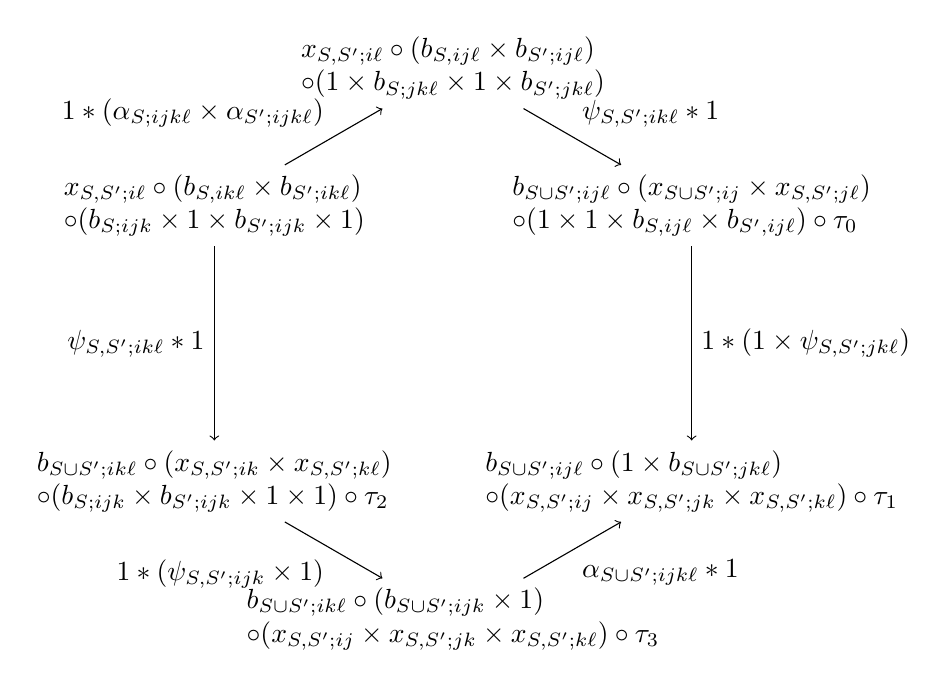
\begin{tikzpicture}[align=left]
	%		\node (A) at (126:2cm) {A};
	%		\node (B) at (54:2cm) {B};
	%		\node (C) at (342:2cm) {C}; % -18 degrees
	%		\node (D) at (270:2cm) {D};
	%		\node (E) at (198:2cm) {E};		
			\node  (A) at (150:3.5cm) {$x_{S, S'; i\ell} \circ (b_{S, ik\ell} \times b_{S'; ik\ell})$ \\ $\circ (b_{S; ijk} \times 1 \times b_{S'; ijk} \times 1)$};
			\node (B) at (90:3.5cm) {$x_{S, S'; i\ell} \circ (b_{S, ij\ell} \times b_{S'; ij\ell})$\\ $ \circ (1 \times b_{S; jk\ell} \times 1 \times b_{S'; jk\ell})$};
			\node (C) at (30:3.5cm) {$b_{S\cup S'; ij\ell} \circ (x_{S\cup S'; ij} \times x_{S, S'; j\ell}) $\\ $ \circ (1 \times 1 \times b_{S, ij\ell} \times b_{S', ij\ell} ) \circ \tau_0$}; 
			\node (D) at (330:3.5cm) {$b_{S\cup S'; ij\ell} \circ (1 \times b_{S \cup S'; jk\ell}) $\\ $ \circ (x_{S, S'; ij} \times x_{S, S'; jk} \times x_{S, S'; k\ell}) \circ \tau_1$};
			\node (E) at (270:3.5cm) {$b_{S \cup S'; ik\ell} \circ (b_{S \cup S';ijk} \times 1) $\\$ \circ (x_{S, S'; ij} \times x_{S, S'; jk} \times x_{S, S'; k\ell}) \circ \tau_3$};
			\node (F) at (210:3.5cm) {$b_{S \cup S'; ik\ell} \circ (x_{S, S'; ik} \times x_{S, S'; k \ell}) $\\$ \circ (b_{S;ijk} \times b_{S';ijk} \times 1 \times 1) \circ \tau_2$};
			\draw [->] (A) to node [above left] {$1*(\alpha_{S; ijk\ell} \times \alpha_{S'; ijk\ell})$} (B);
			\draw [->] (B) to node [above right] {$\psi_{S, S'; ik\ell}*1$} (C);
			\draw [->] (C) to node [right] {$1 * (1 \times \psi_{S,S'; jk\ell})$} (D);
			\draw [->] (A) to node [left] {$\psi_{S, S'; ik\ell}*1$} (F);
			\draw [->] (F) to node [below left] {$1 * (\psi_{S,S'; ijk} \times 1)$} (E);
			\draw [->] (E) to node [below right] {$\alpha_{S \cup S';ijk\ell} * 1$} (D);
		\end{tikzpicture}
	\end{center}
	\label{fig:EqnSSijkObject}
\end{figure}
where each $\tau_i$ represents an appropriate permutation of the factors. In other words, $(x_{S,S';-}, \psi_{S, S'; -})$ forms a structure analogous to a functor of bicategories. 
	\item  For every triple of disjoint subsets $S, S', S''$ and every 2-simplex $ijk$, the  `hexagon' equation in Figure \ref{fig:EqnSSSijObject} holds.
	\begin{figure}[ht]
		\caption{Equation for condition (TCO6) on the data of an object of $\TC(A,n)$.}
	\begin{center}
		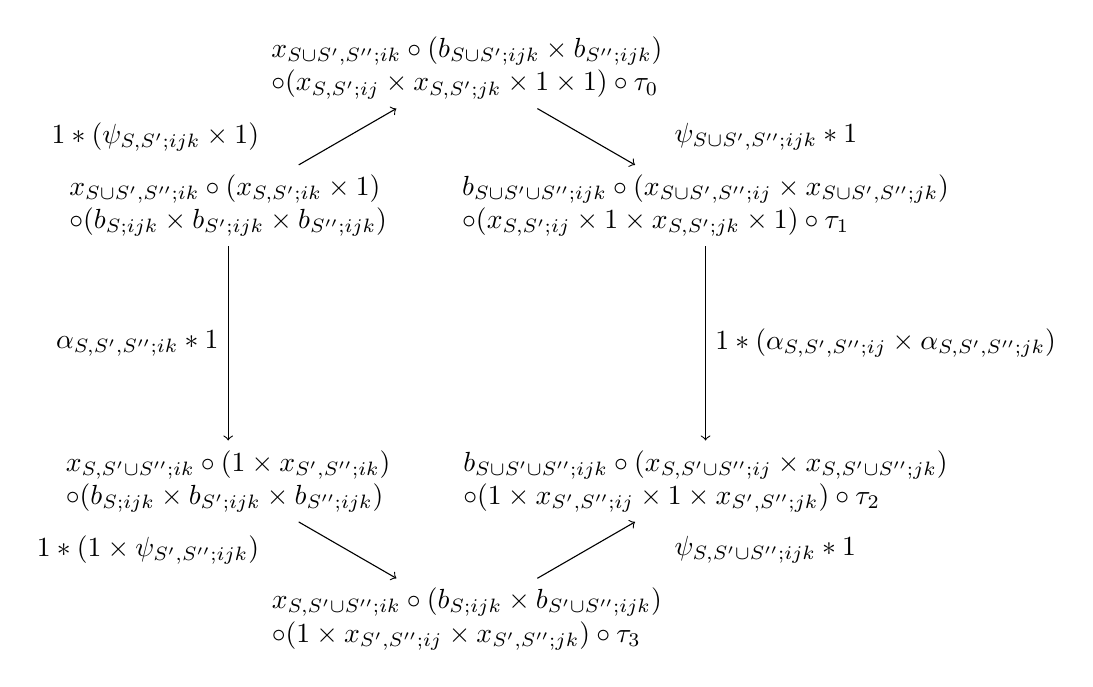
\begin{tikzpicture}[align=left]
	%		\node (A) at (126:2cm) {A};
	%		\node (B) at (54:2cm) {B};
	%		\node (C) at (342:2cm) {C}; % -18 degrees
	%		\node (D) at (270:2cm) {D};
	%		\node (E) at (198:2cm) {E};		
			\node (A) at (150:3.5cm) {$x_{S \cup S', S'';ik} \circ (x_{S, S'; ik} \times 1) $\\$\circ (b_{S;ijk} \times b_{S';ijk} \times b_{S'';ijk})$};
			\node (B) at (90:3.5cm) {$x_{S \cup S', S'';ik} \circ (b_{S\cup S'; ijk} \times b_{S''; ijk}) $\\$ \circ (x_{S, S'; ij} \times x_{S, S'; jk} \times 1 \times 1) \circ \tau_0$};
			\node (C) at (30:3.5cm) {$b_{S \cup S' \cup S''; ijk} \circ (x_{S \cup S', S''; ij} \times x_{S \cup S', S''; jk}) $\\$ \circ (x_{S, S'; ij} \times 1 \times x_{S, S'; jk} \times 1 ) \circ \tau_1$}; 
			\node (D) at (330:3.5cm) {$b_{S \cup S' \cup S''; ijk} \circ (x_{S , S' \cup S''; ij} \times x_{S,  S'\cup S''; jk}) $\\$ \circ ( 1 \times x_{S', S''; ij} \times 1 \times x_{S', S''; jk}) \circ \tau_2$};
			\node (E) at (270:3.5cm) {$x_{S, S' \cup S'';ik} \circ (b_{S;ijk} \times b_{S' \cup S''; ijk}) $\\$ \circ (1 \times x_{S', S'';ij} \times x_{S', S''; jk})  \circ \tau_3$};
			\node (F) at (210:3.5cm) {$x_{S, S' \cup S'';ik} \circ (1 \times x_{S', S''; ik} ) $\\$ \circ (b_{S;ijk} \times b_{S';ijk} \times b_{S'';ijk})$};
			\draw [->] (A) to node [left=1cm] {$1* (\psi_{S, S';ijk}\times 1)$} (B);
			\draw [->] (B) to node [right=1cm] {$\psi_{S\cup S', S''; ijk} * 1$} (C);
			\draw [->] (C) to node [right] {$1 * (\alpha_{S,S',S''; ij} \times \alpha_{S, S', S''; jk})$} (D);
			\draw [->] (A) to node [left] {$\alpha_{S, S', S'';ik}*1$} (F);
			\draw [->] (F) to node [ left=1cm] {$1 * (1 \times \psi_{S', S''; ijk})$} (E);
			\draw [->] (E) to node [right=1cm] {$\psi_{S, S' \cup S''; ijk}*1$} (D);
		\end{tikzpicture}
	\end{center}
		\label{fig:EqnSSSijObject}
	\end{figure}
	where $\tau_i$ is an appropriate permutation of the factors. 
	\item  For every quadruple of disjoint subsets $S, S', S'', S'''$, $\alpha_{-; i}$ and $\alpha_{-; ij}$ satisfy the evident pentagon equations. When $S' = \emptyset$ then $\alpha_{S, S', S''; i}$ and $\alpha_{S, S', S''; ij}$ satisfy the evident triangle identity. 
\end{list}

Let $X$ and $Y$ be two objects in $\TC(A,n)$. A 1-morphism from $X$ to $Y$ may only exist if each of the tensor categories agree identically $X_{S;i} = Y_{S;i}$ for each subset $S \subseteq A$ and vertex $i$ of $[n]$. In this case the 1-morphisms from $X$ to $Y$ consist of collections of data as in Table \ref{Table:1MorOfTC}.
\begin{table}[h]
	\caption{Data of a 1-morphism of $\TC(A,n)$.}
	\begin{tabular}{c |cccc}
	 subsets \textbackslash\ faces & vertex $i$ & edge $ij$ & 2-simplex $ijk$ & 3-simplex $ijk\ell$  \\
	\hline
	$S$ 				& n/a & $F_{S; ij}$ & $\xi_{S; ijk}$  &  (TC1M2) \\
	$S, S'$ 			& n/a & $\varphi_{S, S';ij}$ &  (TC1M3) & \\
	$S, S', S''$ 		& n/a  & (TC1M4) & & \\
	\end{tabular}
	
	\vspace{0.5cm}
	
	\begin{tabular}{l p{11cm}}
		datum & description of datum \\ \hline
		$F_{S;ij}$ & An $X_{S;i}$-$X_{S;j}$-bimodule functor from $X_{S;ij}$ to $Y_{S;ij}$. \\
		$\xi_{S;ijk}$ & A natural isomorphism of $X_{S;j}$-balanced $X_{S;i}$-$X_{S;k}$-bimodule functors from $b^Y_{S;ijk} \circ (F_{S;ij} \times F_{S; jk})$ to $F_{S;ik} \circ b^X_{S;ijk}$. \\
		$\varphi_{S,S'; ij}$ & A natural isomorphism of bilinear bimodule functors from $y_{S,S'; ij} \circ (F_{S; ij} \times F_{S';ij})$ to $F_{S \cup S'; ij} \circ x_{S, S'; ij}$. 
	\end{tabular}
	\label{Table:1MorOfTC}
\end{table}
This data is required to satisfy the following axioms:
\begin{list}{(TC1M\arabic{itemcounter})}{\usecounter{itemcounter}}
	\item If $S = \emptyset$, the $F_S;ij$ and $\xi_{S;ijk}$ are identities. If either $S$ or $S'$ is equal to $\emptyset$, then $\varphi_{S,S';ij}$ is the canonical map.
	\item For every subset $S$ and every 3-simplex $ijk\ell$ the hexagon equation in Figure \ref{fig:EqnSijklMorphism} holds.
	\begin{figure}[ht]
		\caption{Equation for condition (TC1M2) on the data of a 1-morphism of $\TC(A,n)$.}
		\begin{center}
			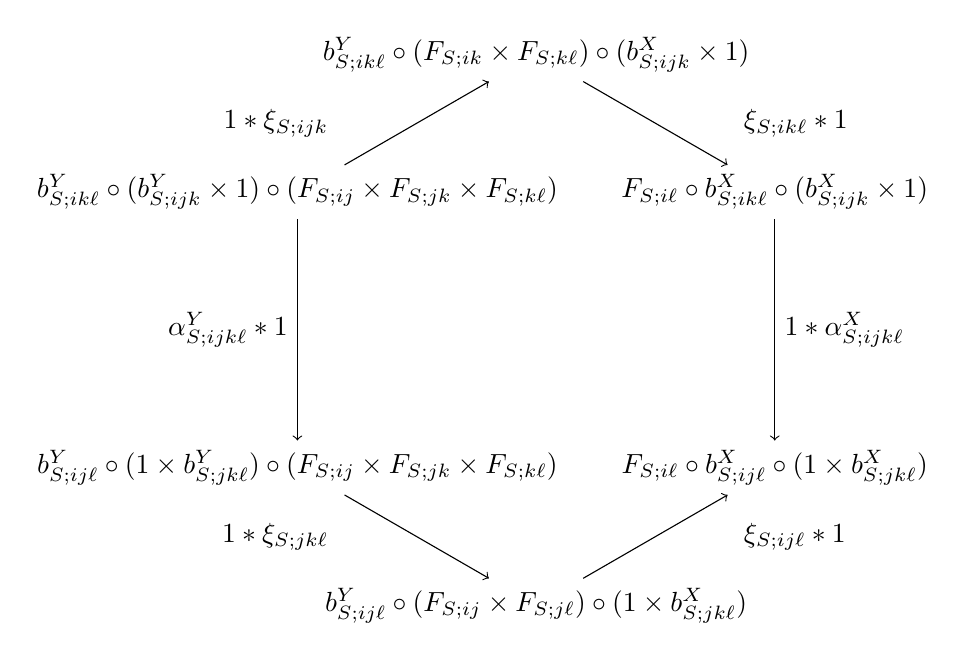
\begin{tikzpicture}[align=left]	
				\node (A) at (150:3.5cm) {$b^Y_{S;ik\ell} \circ (b^Y_{S;ijk} \times 1) \circ (F_{S;ij} \times F_{S;jk} \times F_{S;k\ell})$};
				\node (B) at (90:3.5cm) {$b^Y_{S;ik\ell} \circ (F_{S;ik} \times F_{S;k\ell}) \circ (b^X_{S;ijk} \times 1) $};
				\node (C) at (30:3.5cm) {$F_{S;i\ell} \circ b^X_{S;ik\ell} \circ (b^X_{S;ijk} \times 1)$}; 
				\node (D) at (330:3.5cm) {$F_{S;i\ell} \circ b^X_{S;ij\ell} \circ (1 \times b^X_{S;jk\ell})$};
				\node (E) at (270:3.5cm) {$b^Y_{S;ij\ell} \circ (F_{S;ij} \times F_{S;j\ell}) \circ (1 \times b^X_{S;jk\ell}) $};
				\node (F) at (210:3.5cm) {$b^Y_{S;ij\ell} \circ (1 \times b^Y_{S;jk\ell})  \circ (F_{S;ij} \times F_{S;jk} \times F_{S;k\ell})$};
				\draw [->] (A) to node [left=1cm] {$1*\xi_{S;ijk}$} (B);
				\draw [->] (B) to node [right=1cm] {$\xi_{S; ik\ell} * 1$} (C);
				\draw [->] (C) to node [right] {$1*\alpha^X_{S;ijk\ell}$} (D);
				\draw [->] (A) to node [left] {$\alpha^Y_{S;ijk\ell} * 1$} (F);
				\draw [->] (F) to node [ left=1cm] {$1*\xi_{S;jk\ell}$} (E);
				\draw [->] (E) to node [right=1cm] {$\xi_{S; ij\ell}*1$} (D);
			\end{tikzpicture}
		\end{center}
		\label{fig:EqnSijklMorphism}
	\end{figure}
	\item For every pair of disjoint subsets $S, S'$ and every 2-simplex $ijk$ the hexagon equation in Figure \ref{fig:EqnSSijkMorphism} holds, where $\tau$ permutes the middle factors. 
	\begin{figure}[ht]
		\caption{Equation for condition (TC1M3) on the data of a 1-morphism of $\TC(A,n)$.}
		\begin{center}
			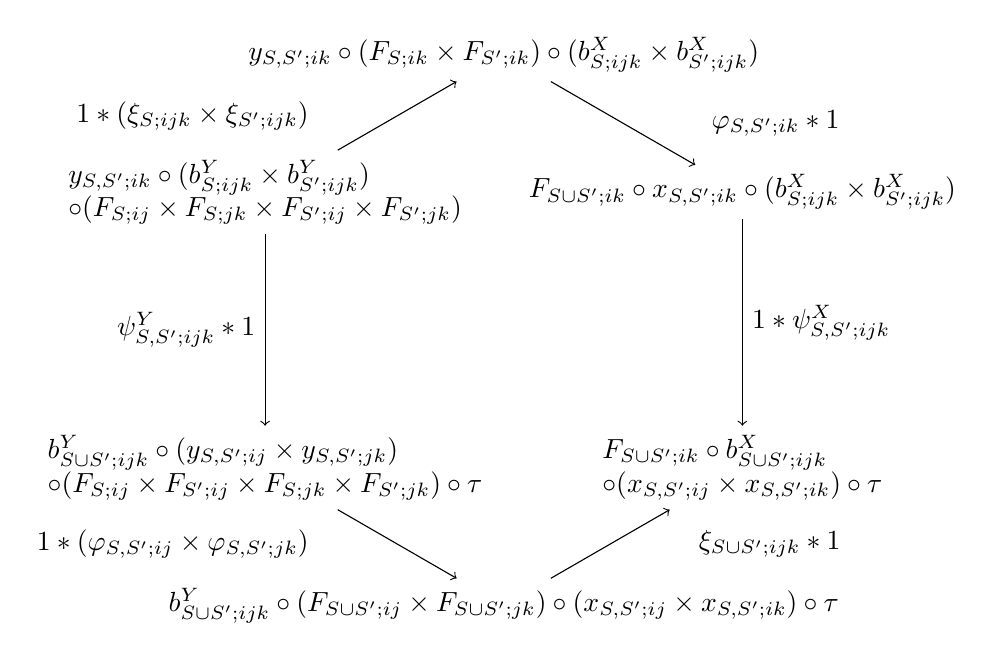
\begin{tikzpicture}[align=left]	
				\node (A) at (150:3.5cm) {$y_{S, S'; ik} \circ (b^Y_{S; ijk} \times b^Y_{S';ijk}) $\\$ \circ (F_{S; ij} \times F_{S; jk} \times F_{S'; ij} \times F_{S'; jk})$};
				\node (B) at (90:3.5cm) {$y_{S, S'; ik} \circ (F_{S; ik} \times F_{S'; ik}) \circ (b^X_{S;ijk} \times b^X_{S'; ijk}) $};
				\node (C) at (30:3.5cm) {$F_{S \cup S'; ik} \circ x_{S, S'; ik} \circ (b^X_{S;ijk} \times b^X_{S'; ijk})$}; 
				\node (D) at (330:3.5cm) {$F_{S \cup S'; ik} \circ b^X_{S \cup S'; ijk} $\\$ \circ (x_{S,S'; ij} \times x_{S,S'; ik}) \circ \tau$};
				\node (E) at (270:3.5cm) {$ b^Y_{S \cup S'; ijk} \circ (F_{S \cup S'; ij} \times F_{S \cup S'; jk}) \circ (x_{S,S'; ij} \times x_{S,S'; ik}) \circ \tau$};
				\node (F) at (210:3.5cm) {$ b^Y_{S \cup S'; ijk} \circ (y_{S,S'; ij} \times y_{S, S'; jk}) $\\$  \circ (F_{S; ij} \times F_{S'; ij} \times F_{S; jk}  \times F_{S'; jk}) \circ \tau$};
				\draw [->] (A) to node [left=1cm] {$1* (\xi_{S;ijk} \times \xi_{S';ijk})$} (B);
				\draw [->] (B) to node [right=1cm] {$\varphi_{S,S';ik}*1$} (C);
				\draw [->] (C) to node [right] {$1* \psi^X_{S, S'; ijk}$} (D);
				\draw [->] (A) to node [left] {$\psi^Y_{S, S'; ijk} * 1$} (F);
				\draw [->] (F) to node [ left=1cm] {$1* (\varphi_{S, S'; ij} \times \varphi_{S, S'; jk})$} (E);
				\draw [->] (E) to node [right=1cm] {$\xi_{S \cup S'; ijk}*1$} (D);
			\end{tikzpicture}
		\end{center}
		\label{fig:EqnSSijkMorphism}
	\end{figure} 
	\item For every triple of disjoint subsets $S, S', S''$ and every edge $ij$, the hexagon equation in Figure \ref{fig:EqnSSSijMorphism} holds.
	\begin{figure}[ht]
		\caption{Equation for condition (TC1M4) on the data of a 1-morphism of $\TC(A,n)$.}
		\begin{center}
			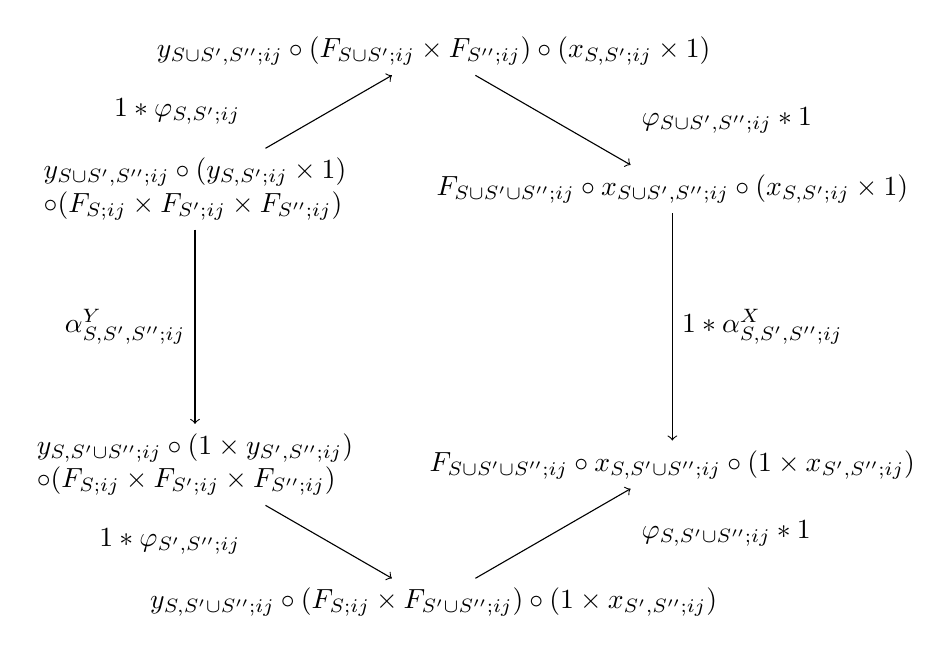
\begin{tikzpicture}[align=left]	
				\node (A) at (150:3.5cm) {$y_{S \cup S', S''; ij} \circ (y_{S, S'; ij} \times 1) $\\$ \circ (F_{S; ij} \times F_{S'; ij} \times F_{S''; ij})$};
				\node (B) at (90:3.5cm) {$y_{S \cup S', S''; ij} \circ (F_{S \cup S'; ij} \times F_{S'';ij}) \circ (x_{S,S';ij} \times 1) $};
				\node (C) at (30:3.5cm) {$F_{S \cup S' \cup S''; ij} \circ x_{S \cup S', S''; ij} \circ (x_{S,S';ij} \times 1)$}; 
				\node (D) at (330:3.5cm) {$F_{S \cup S' \cup S''; ij} \circ x_{S, S'\cup S''; ij} \circ (1 \times x_{S',S'';ij})$};
				\node (E) at (270:3.5cm) {$y_{S,  S'\cup S''; ij} \circ (F_{S;ij} \times F_{S' \cup S''; ij}) \circ (1 \times x_{S', S'';ij}) $};
				\node (F) at (210:3.5cm) {$y_{S,  S'\cup S''; ij} \circ (1 \times y_{S', S''; ij}) $\\$ \circ (F_{S; ij} \times F_{S'; ij} \times F_{S''; ij})$};
				\draw [->] (A) to node [left=1cm] {$1*\varphi_{S,S';ij}$} (B);
				\draw [->] (B) to node [right=1cm] {$\varphi_{S\cup S', S''; ij}*1$} (C);
				\draw [->] (C) to node [right] {$1 * \alpha^X_{S,S', S''; ij}$} (D);
				\draw [->] (A) to node [left] {$\alpha^Y_{S, S', S'';ij}$} (F);
				\draw [->] (F) to node [ left=1cm] {$1 * \varphi_{S', S''; ij}$} (E);
				\draw [->] (E) to node [right=1cm] {$\varphi_{S, S' \cup S''; ij}*1$} (D);
			\end{tikzpicture}
		\end{center}
		\label{fig:EqnSSSijMorphism}
	\end{figure}
\end{list}
A 2-morphism between 1-morphisms $F$ and $G$ from $X$ to $Y$ consists of a collection of $\{ \theta_{S;ij} \}$ consisting of $X_{S;i}$-$X_{S;j}$-bimodule natural transformations from $F_{S;ij}$ to $G_{S;ij}$ for each subset $S \subseteq A$ and 2-simplex $ij$ in $[n]$. For completeness we record this in Table \ref{Table:2MorOfTC}.
\begin{table}[h]
	\caption{Data of a 2-morphism of $\TC(A,n)$.}
	\begin{tabular}{c |ccc}
	 subsets \textbackslash\ faces & vertex $i$ & edge $ij$ & 2-simplex $ijk$   \\
	\hline
	$S$ 				& n/a & $\theta_{S; ij}$ &     (TC2M1) \\
	$S, S'$ 			& n/a &  (TC2M2)  &    \\
	\end{tabular}
%	
%	\vspace{0.5cm}
%	
%	\begin{tabular}{l p{11cm}}
%		datum & description of datum \\ \hline
%		$\theta_{S;ij}$ & An $X_{S;i}$-$X_{S;j}$-bimodule natural transformation from $X_{S;ij}$ to $Y_{S;ij}$. 
%	\end{tabular}
	\label{Table:2MorOfTC}
\end{table}
These are required to satisfy that $\theta_{\emptyset;ij}$ is the identity and the following pair of equations hold:
\begin{list}{(TC2M\arabic{itemcounter})}{\usecounter{itemcounter}}
	\item For each 2-simplex $ijk$, we have
	\begin{equation*}
		(\theta_{S; ik} * 1) \circ \xi^F_{S; ijk} = xi^G_{S;ijk} \circ (1 * (\theta_{S; ij} \times \theta_{S; jk})).
	\end{equation*}
	\item For each pair of disjoint subsets $S, S'$ we have
	\begin{equation*}
		(\theta_{S \cup S'; ij} * 1) \circ \varphi^F_{S, S'; ij} = \varphi^G_{S,S';ij} \circ (1*(\theta_{S;ij} \times \theta_{S';ij})).
	\end{equation*}
\end{list}
With these as objects, 1-morphisms, and 2-morphisms, the obvious composition makes $\TC(A,n)$ into a strict $2$-category. It is manifestly functorial in $A$ and $[n]$ and thus gives a (strict) functor 
\begin{equation*}
	\TC: \Gamma^\textrm{op} \times \Delta^\textrm{op} \to \Cat_2.
\end{equation*}
into the 1-category of strict 2-categories. Composing with the coherent nerve for strict 2-categories gives us a $\Gamma$-3-fold simplicial space, which we also denote $\TC$.

\begin{theorem}
	 $\TC$ is a symmetric monoidal 3-fold Segal category.  
\end{theorem}

\CSP{This maybe needs a little more explanation...}
\begin{proof}
	By Lemma \ref{lma:2catnervereflectsequiv} it is enough to show that the functor to strict 2-categories satisfies the appropriate Segal conditions, i.e. that the following Segal maps are weak equivalences of strict 2-categories:
	\begin{align*}
		\TC(A, m + n) & \to \TC(A, m) \times_{\TC(A, 0)} \TC(A, n), \\
		\TC(A, n) & \to \TC(1, n)^{\times |A|}. 
	\end{align*}
However $\TC$ is constructed in such a way that these Segal maps are manifestly weak equivalences. In each case the difference between the left-hand-side and the right-hand-side consists of choices of representatives of a Deligne tensor product (and maps representing the tensor product). The category of such choices is contractible (by the universal property of the Deligne tensor product) hence these Segal maps are equivalences. 
\end{proof}
 

\CSPcomm{Now maybe set up notion that will be used later in the paper? eg variations on TC, hom categories, etc?}


\section{Local Field Theory in Dimension Three} \label{sec-lft}

\subsection{Dualizability in 3-categories} \label{sec-lft-dual}
.
\CD{I guess the content of this section should be dictated by what we need for sections 4,5,6.  What is that?}

[Adjunction convention: $\bimod{C}{M}{D} \adj  \bimod{D}{N}{C}$ if there are $M \dtimes_D N \ra C$ and $D \ra N \dtimes_C M$ satisfying the S relations.] 

\CSPcomm{Set up terminology for evaluation and coevaluation.}


%\CSP{This proposition is stated as a remark, without proof in Jacob's paper.}

\begin{proposition}[Lurie, Remark 3.4.22] \label{prop-ambiadjoints}
	Let $\cA$ be a symmetric monoidal 3-category. Let $f: x \to y$ be a 1-morphism in $\cA$, and suppose that $f$ admits a right adjoint $f^R$,  so we have unit and counit maps $u:id_x \to f^R \circ f$ and $v:f \circ f^R \to id_y$. If $u$ and $v$ admit left adjoints $u^L$ and $v^L$, then $u^L$ and $v^L$ exhibit $f^R$ also as a left adjoint to $f$. 
\end{proposition}

\begin{proof}
\CDcomm{[Should we include a proof?]} \CSPcomm{Of Course we should include a proof. Jacob omits one, so there is none in the literature, plus we need it as a substitute for the cob hypothesis for our applications to finite tensor cats.}

By assumption we are given 3-morphisms,
\begin{align*}
	\varepsilon_v: v^L \circ v & \Rightarrow id_{f \circ f^R} \\
	\eta_v: id_{id_y} & \Rightarrow v \circ v^L \\
	\varepsilon_u: u^L \circ u & \Rightarrow id_{id_x} \\
	\eta_u: id_{f^R \circ f} & \Rightarrow  u \circ u^L
\end{align*}
which satisfy the Zig-Zag identities:
\begin{align*}
	 id_v  &= (id_v * \varepsilon_v) \circ (\eta_v * id_v)  \\
	 id_{v^L}  &= (\varepsilon_v * id_{v^L} ) \circ (id_{v^L} * \eta_v)  \\
	 id_u  &= (id_u * \varepsilon_u) \circ (\eta_u * id_u)  \\
	 id_{u^L}  &= (\varepsilon_u * id_{u^L} ) \circ (id_{u^L} * \eta_u).  
\end{align*}
We must show that the following Zig-Zag identities hold:
\begin{align*}
	 (id_{f} * u^L) \circ (v^L * id_{f} ) & \cong id_{f} \\
 	 (u^L * id_{f^R}) \circ (id_{f^R} * v^L) & \cong id_{f^R} 
\end{align*}
By assumption we may also choose isomorphisms as follows:
\begin{align*}
	\alpha: id_f &\stackrel{\cong}{\to} (v * id_f) \circ (id_f * u) \\
	\beta: id_{f^R} &\stackrel{\cong}{\to} (id_{f^R} * v) \circ (u * id_{f^R} ).
\end{align*}
Then the required isomorphisms are given by the following composites:
\begin{align*}
	(id_{f} * u^L) \circ (v^L * id_{f} )
		& \cong id_f \circ (id_{f} * u^L) \circ (v^L * id_{f} ) \\
		& \stackrel{\alpha}{\cong} (v * id_f) \circ (id_f * u) \circ (id_{f} * u^L) \circ (v^L * id_{f} ) \\
		&  \stackrel{\varepsilon_u }{\Rightarrow} (v * id_f) \circ (v^L * id_{f} ) \\
		& \stackrel{\varepsilon_v }{\Rightarrow} id_{f},  \\
	(u^L * id_{f^R}) \circ (id_{f^R} * v^L) 
		& \cong  id_{f^R} \circ (u^L * id_{f^R}) \circ (id_{f^R} * v^L)  \\
		& \stackrel{\beta}{\cong}  (id_{f^R} * v) \circ (u * id_{f^R} )  \circ (u^L * id_{f^R}) \circ (id_{f^R} * v^L) \\
		& \stackrel{\varepsilon_u }{\Rightarrow} (id_{f^R} * v) \circ (id_{f^R} * v^L) \\
		& \stackrel{\varepsilon_v }{\Rightarrow} id_{f^R}.
\end{align*}
\end{proof}

In particular, if you are in a situation where you happen to know a priori that the 2-morphisms $u$ and $v$ will have left adjoints, then you know that any adjoint to the 1-morphism $f$ will be ambidextrous.  % This proposition gets used in the Remark in the section computing the Serre automorphism.

\subsection{Structure groups of 3-manifolds} \label{sec-lft-struc}

\begin{definition}
An \emph{structure} for $n$-dimensional vector bundles is a space $T$ together with a fibration $f: T \ra BO(n)$.  A $T$-structure on an n-dimensional vector bundle $V$ on $X$ is a lift of the classifying map $X \xra{V} BO(n)$ along $f$ to $T$.
\end{definition}

We will be primarily interested in five structures for 3-dimensional vector bundles, namely \emph{orientation}, \emph{combing}, \emph{oriented $p_1$ structure}, \emph{quadratic structure}, and \emph{framing}.  The structure spaces for an orientation, combing, and framing are respectively $BSO(3)$, $BSO(2)$, and $BSO(1) = *$, all with the obvious maps to $BO(3)$.  The structure spaces for oriented $p_1$ structure and quadratic structure are as follows:
\begin{definition}
The following two spaces, together with the obvious maps to $BO(3)$, define the aforementioned bundle structures:
\begin{itemize}
\item[Orpo:] $BOrpo(3) := \hofib(BSO(3) \ra BSO \xra{p_1} K(\ZZ,4))$
\item[Quad:] $BQuad := \hofib(BSO(2) = BU(1) \xra{c_1^2} K(\ZZ,4))$
\end{itemize}
\end{definition}

\begin{remark}
``Orpo structure" is short for ``oriented $p_1$ structure", and sometimes goes under the name ``$p_1$ structure" in the literature.  We reserve the name "$p_1$ structure" for the structure group where only $p_1$ has been killed, rather than $w_1$ and $p_1$.  The terminology "quadratic" refers to the fact that the single k-invariant of the structure space $BQuad$ is the fundamental quadratic map.
\end{remark}

[discussion: recall meaning of 4-type and 4-equivalence, 3.5-equivalence; sufficient to understand 4-type of the structure spaces.  cf wave]

We now precisely identify the 4-homotopy type of the structure spaces under consideration.  The framing structure space is of course contractible.  The homotopy type of the combing structure space is simply $K(\ZZ,2)$, so in particular that is also its 4-type.

\begin{proposition}
The following fibrations consistute the Postnikov towers of the 4-homotopy types of the structure spaces $BSO(3)$, $BOrpo(3)$, and $BQuad$.
\begin{align}
K(\ZZ,4) \ra & \; BSO(3) \ra K(\ZZ/2,2) \overset{\gamma}{\dashrightarrow} K(\ZZ,5) \nn \\
K(\ZZ/4,3) \ra & \; BOrpo(3) \ra K(\ZZ/2,2) \overset{\delta}{\dashrightarrow} K(\ZZ/4,4) \nn \\
K(\ZZ,3) \ra & \; BQuad \ra K(\ZZ,2) \overset{c_1^2}{\dashrightarrow} K(\ZZ,4) \nn
\end{align}
\nid Here the dashed arrow indicates the k-invariant of the preceding fibration.  The class $\delta \in H^4(K(\ZZ/2,2);\ZZ/4)$ is a generator, and the class $\gamma \in H^5(K(\ZZ/2,2);\ZZ) = \ZZ/4$ is, up to sign, the integral Bockstein of $\delta$. \CD{Surely that sign is $+1$; easy way to see that?}
\CSP{You can take it to be either one. You can always compose with an automorphism of $K(\ZZ,5)$, and this switches the two posibilities.}
\end{proposition}

\begin{proof}
The quadratic structure group is defined as the homotopy fiber of the square of the first chern class, so in that case there is nothing to prove.

The first four homotopy groups of $BSO(3)$ are $\pi_1 = 0$, $\pi_2 = \ZZ/2$, $\pi_3 = 0$, $\pi_4 = \ZZ$.  The Postnikov tower of the 4-type of $BSO(3)$ is therefore as indicated for some k-invariant in $H^5(K(\ZZ/2,2);\ZZ) = \ZZ/4$.  This k-invariant isn't trivial: the cohomology group $H^5(K(\ZZ/2,2) \times K(\ZZ,4);\ZZ)$ has 4-torsion elements, while the group $H^5(BSO(3);\ZZ)$ does not.  Similarly, the k-invariant isn't twice a generator of $H^5(K(\ZZ/2,2);\ZZ)$: the group $H^4(K(\ZZ/2,2) \ltimes_{2\gamma} K(\ZZ,4);\ZZ/2)$ is rank two, while $H^4(BSO(3);\ZZ/2)$ is rank one.  The k-invariant for the 4-type of $BSO(3)$ is therefore a generator, as claimed.

The structure space $BOrpo(3)$ is defined as the homotopy fiber of the composite $BSO(3) \ra BSO \xra{p_1} K(\ZZ,4)$; as before we refer to this composite simply as $p_1$.  In the appendix, it is shown that this map $p_1: BSO(3) \ra K(\ZZ,4)$ is a generator of $H^4(BSO(3);\ZZ)$, and, somewhat non-obviously, that it induces multiplication by \emph{four} in homotopy.  The first four homotopy groups of $BOrpo(3)$ are therefore $\pi_1 = 0$, $\pi_2 = \ZZ/2$, $\pi_3 = \ZZ/4$, $\pi_4 = 0$.  The Postnikov tower of the 4-type of $BOrpo(3)$ is therefore as indicated for some k-invariant in $H^4(K(\ZZ/2,2);\ZZ/4) = \ZZ/4$.  The Postnikov tower of a space is functorial, so the existence of a map $BOrpo(3) \ra BSO(3)$ inducing an isomorphism on $pi_2$ forces the k-invariant of $BOrpo(3)$ to be a generator $\delta \in H^4(K(\ZZ/2,2);\ZZ/4)$, and in fact shows that $\pm \beta_{\ZZ} \delta = \gamma$. \CD{The Postnikov tower is functorial, right?} \CSP{Yes, it is functorial.} \CD{Probably that proof could be improved, it's just the first thing that came to mind as I was typing.}
\end{proof}

We have the following diagram of structure spaces:
\begin{equation} \nn
\xymatrix{
BQuad_{K(\ZZ,2)}^{K(\ZZ,3)} \ar[r] \ar[d] & BSO(2)_{K(\ZZ,2)} \ar[d] \\
BOrpo(3)_{K(\ZZ/2,2)}^{K(\ZZ/4,3)} \ar[r] & BSO(3)_{K(\ZZ/2,2)}^{K(\ZZ,4)}
}
\end{equation}
Here we have indicated in the subscripts and superscripts the stages of the respective Postnikov towers of the homotopy 4-types.  The two horizontal maps exist by definition, and the righthand vertical map is the standard inclusion.  The lefthand vertical map may be constructed as follows.  At the first layer of the Postnikov tower, the map $\pi: K(\ZZ,2) \ra K(\ZZ/2,2)$ is induced by the projection $\ZZ \ra \ZZ/2$.  To produce a map $BQuad \ra BOrpo(3)$ it suffices to factor the composite $K(\ZZ,2) \xra{\pi} K(\ZZ/2,2) \xra{\delta} K(\ZZ/4,4)$ through the map $K(\ZZ,2) \xra{c_1^2} K(\ZZ,4)$; this is accomplished by (plus or minus) the projection $K(\ZZ,4) \ra K(\ZZ/4,4)$.  %%% {This is because the path loop construction is functorial so any map K(\ZZ,4) \ra K(\ZZ/4,4) induces a map of fibrations, which pulls back across c_1^2, resp \delta, to give a map of fibrations whose total spaces are BQuad and BOrpo(3) respectively.  To check the factorization, just look at the induced maps in cohomology.

By construction, the four maps of structure spaces above induce the `obvious' maps on homotopy, namely $\pi_2(BQuad \ra BSO(2))$ is the identity, $\pi_2(BQuad \ra BOrpo(3))$ and $\pi_3(BQuad \ra BOrpo(3))$ are both the standard projections, $\pi_2(BSO(2) \ra BSO(3))$ is the standard projection, and $\pi_2(BOrpo(3) \ra BSO(3))$ is the identity.  \CD{This paragraph is stated on the nose, whereas previous statements were up to sign.  Should fix this.}




\section{Dualizability and tensor categories} \label{sec-dualfusion}


\subsection{Adjoints of bimodule functors} \label{sec-df-functors}

In this section we give sufficient conditions for a bimodule functor $\cF: {}_\cC \cM_\cD \rightarrow {}_\cC \cN_\cD$ to have a left adjoint and a right adjoint.  In particular, we show that any module functor between semisimple module categories over fusion categories has a left adjoint and a right adjoint.

\begin{lemma} \label{module-adjoint}
Let $\cC, \cD \in \TCrig$, let $\cC \cM, \cN \in \Hom_\TCrig(\cC,\cD)$, and let $\cF \in \Hom_{\TCrig}(\cM,\cN)$.  If the underlying functor of $\cF$ has a right (or left) adjoint as a functor, then $\cF$ has a right (resp. left) adjoint in $\Hom_{\TCrig}(\cN,\cM)$.
\end{lemma}
\begin{proof}
Suppose that $\cG$ is the right adjoint to the underlying functor of $\cF$, we will show that $\cG$ has a natural structure of a $\cC\boxtimes \cD^{mp}$-module functor.  The result for left adjoints is similar.

The binatural transformation $\psi_{x,n}: x \otimes \cG(n) \rightarrow \cG(x \otimes n)$ is given by
$$x \otimes \cG(n) \rightarrow \cG \cF(x \otimes \cG(n)) \rightarrow \cG(x \otimes \cF\cG(n)) \rightarrow \cG(x \otimes n)$$
where the first map is the unit of the adjunction, the second map is the binatural transformation coming from the module functor structure on $\cF$ and the third map is the counit.  Rigidity of $\cC$ and $\cD$ guarantees that this binatural transformation is an isomorphism.  The compatibility condition is an easy exercise with commuting diagrams.
\end{proof}

\begin{remark}
If $\cC$ and $\cD$ are not rigid the above argument only shows that the right adjoint to a lax module functor has an oplax module functor structure, while the left adjoint of an oplax module functor has a lax module functor structure.  
\end{remark}


\begin{proposition} \cite{???}
If $\cB$ is a finite tensor category and $\cM$ and $\cN$ are module categories over $\cB$ with $\cM$ exact, then any module category functor $\cF:\cM \rightarrow \cN$ is exact.
\end{proposition}

\begin{corollary}
Let $\cC, \cD \in \TCrig$, let $\cM, \cN \in \Hom_\TCrig(\cC,\cD)$, and let $\cF \in \Hom_{\TCrig}(\cM,\cN)$.  Suppose that $\cB$ is an auxiliary finite tensor category, that $\cM$ and $\cN$ are $\cB$ module categories, and that the underlying functor $\cF$ can be given the structure of a $\cB$ module category.  If $\cM$ is exact as a $\cB$ module category, then $\cF$ has both a left adjoint functor and a right adjoint functor in $\Hom_{\TCrig}(\cN,\cM)$.  
\end{corollary}
\begin{proof}
Exactness of $\cM$ as a $\cB$ module category guarantees that the underlying functor of $\cF$ is exact and thus has both left and right adjoints as a functor.  Then Lemma \ref{module-adjoint} shows that it has left and right adjoints as a $\cC$--$\cD$ bimodule functor.
\end{proof}

\begin{remark}
In applications of the above corollary $\cB$ will typically be $\mathrm{Vec}$, $\cC$, $\cD^{mp}$, or $\cC \boxtimes \cD^{mp}$.
\end{remark}

\begin{corollary}
Any $2$-morphism in $\TCss$ has a left adjoint and a right adjoint in $\TCss$.
\end{corollary}
\begin{proof}
Apply the above corollary with $\cB = \mathrm{Vec}$.
\end{proof}

\subsection{Adjoints of bimodules}  \label{sec-df-modules}

In this section we give sufficient conditions for a  bimodule category ${}_\cC \cM_\cD$ to have left and right adjoints.  In particular, if $\cC$ and $\cD$ are finite tensor categories, and their action on $\cM$ is left exact, then $\cM$ has both a left and a right adjoint.  Explicitly, the right adjoint of of $\cM$ is the category of right exact left module functors $\Fun_{\cC\text{-mod}}(\cM, \cC)$ where the left $\cD$ action is given by precomposition by right multiplication, and the right $\cC$ action is given by postcomposition by right multiplication.  Similarly, the left adjoint is given by the category of right exact right module functors $\Fun_{\text{mod}-\cD}(\cM, \cD)$.  The key assumptions in this section are finiteness of the categories and right exactness of the module actions.

\begin{lemma}
The map $\ev: \Fun_{\text{mod}-\cD}(\cM, \cD) \boxtimes_{\cC} \cM \rightarrow \cD$ induced by the $\cC$-balanced bifunctor $(f,m) \mapsto f(m)$ has a natural $\cD$--$\cD$ bimodule structure given by $f(m d_1) d_2 \mapsto f(m) d_1 d_2$ via the mod-$\cD$ structure on $f$.  Similarly, $\ev: \cM \boxtimes_{\cD} \Fun_{\cC\text{-mod}}(\cM, \cC) \rightarrow \cC$ is naturally a map of $\cC$--$\cC$ bimodule categories.
\end{lemma}
\begin{proof}
Straightforward.
\end{proof}

The maps $\ev$ give the counits of the adjunctions.  The units of the adjunctions are more delicate, since it is more difficult to describe maps into a tensor product than maps out of a tensor product.  In order to describe the units we first give an alternate description of the tensor product as a category of functors.

\begin{lemma}
If ${}_\cC\cM_\cD$ and ${}_\cC \cN_\cE$ are finite bimodule categories where the bimodule actions are right exact, then the map $\Fun_{\cC\text{-mod}}(\cM,\cC) \boxtimes_\cC \cN \rightarrow \Fun_{\cC\text{-mod}}(\cM,\cN)$ induced by $(f,n) \mapsto (m \mapsto f(m)n)$ is an equivalence of $\cD$--$\cE$ bimodules.
\end{lemma}
\begin{proof}
\CSPcomm{This is now lemma \ref{Lma:FunctorsAsATensorPdt}, maybe move that here?}
\end{proof}

\begin{lemma}
The map $\coev: \cD \rightarrow \Fun_{\cC\text{-mod}}(\cM,\cM) \cong \Fun_{\cC\text{-mod}}(\cM,\cC) \boxtimes_\cC \cM$ sending $d$ to right multiplication by $d$ is a map of $\cD$--$\cD$ bimodules.  Similarly, the map $\coev: \cC \rightarrow \Fun_{\text{mod}-\cD}(\cM,\cM) \cong \Fun_{\text{mod}-\cD}(\cM,\cD) \boxtimes_\cD \cM$ sending $c$ to left multiplication by $c$ is a map of $\cC$--$\cC$ bimodules.
\end{lemma}

\begin{theorem}
$\ev$ and $\coev$ are the unit and counit of an adjunction.
\end{theorem}
\begin{proof}
The following diagram commutes.
		\begin{center}
			\begin{tikzpicture}[align=left]	
				\node (A) at (0in,2in) {${}_\cC \cM_\cD$};
				\node (B) at (0in,1.5in) {${}_\cC \cM \boxtimes_\cD \cD_\cD$};
				\node (C) at (0in,1in) {${}_\cC \cM \boxtimes_\cD \Fun_{\cC\text{-mod}}(\cM,\cC) \boxtimes_\cC \cM_\cD$};
				\node (D) at (2in,1.5in) {${}_\cC \cM \boxtimes_D \Fun_{\cC\text{-mod}}(\cM,\cM)_\cD$};
				\node (E) at (0in, .5in) {${}_\cC \cC \boxtimes_\cC \cM_\cD$};
				\node (F) at (0in,0in) {${}_\cC \cM_\cD$};
				\draw [<->] (A) to node [left=.1cm] {} (B);
				\draw [->] (B) to node [left=.1cm] {$\id \boxtimes \coev$}  (C);
				\draw [->] (B) to node [above=.1cm]{$\id \boxtimes (d \mapsto \bullet \otimes d)$} (D);
				\draw [<->] (C) to node {} (D);
				\draw [->] (C) to node [left=.1cm]{$\ev \boxtimes \id$} (E);
				\draw [<->] (E) to node {} (F);
				\draw [->] (D) to node [right=.1cm]{$m \boxtimes \cF \mapsto \cF(m)$} (F);
			\end{tikzpicture}
		\end{center}

Thus instead of computing along the left side of the diagram, we can compute along the right side of the diagram to see that the composition ${}_\cC \cM_\cD \rightarrow {}_\cC \cM_\cD$ is given by right multiplication by $1$, and hence is the identity.

The other three calculations are similar.
\end{proof}


It will sometimes be convenient to have an alternative description of the left and right adjoints to $\cM$.

\begin{definition}
Let ${}^*\cM$ denote the $\cD$--$\cC$ bimodule category whose underlying category is $\cM^{\op}$ and the action is given by $d\cdot m \cdot c = {}^*c \otimes m \otimes {}^*d$.  Similarly, let Let $\cM^*$ denote the $\cD$--$\cC$ bimodule category whose underlying category is $\cM^{\op}$ and the action is given by $d\cdot m \cdot c = c^* \otimes m \otimes d^*$.  
\end{definition}

\begin{lemma}
If $\cM$ is a $\cC$--$\cD$ bimodule category and $\cN$ is a $\cC$--$\cE$ bimodule category, then taking right adjoints gives an equivalence of $\cD$--$\cE$ bimodules $\Fun_{\cC-\text{mod}}(\cM, \cN) \rightarrow {}^*\Fun_{\cC-\text{mod}}(\cN, \cM)$.  Similarly, if $\cM$ is a $\cC$--$\cD$ bimodule category and $\cN$ is a $\cD$--$\cE$ bimodule category, then taking right adjoints gives an equivalence of $\cC$--$\cE$ bimodules $\Fun_{\text{mod}-D}(\cM, \cN) \rightarrow \Fun_{\cC-\text{mod}}(\cN, \cM)^*$. 
\end{lemma}
\begin{proof}
We've already seen that the right adjoint has a canonical module functor structure.  To see that the actions match, note that taking adjoints interchanges precomposition and postcomposition, and the right adjoint of left multiplication by $x$ is left multiplication by ${}^*x$.  For the second statement, note that the right adjoint of right multiplication by $x$ is right multiplication by $x^*$.
\end{proof}

\begin{lemma} \label{lem:dual-formula-for-adjoints}
We have that $\cM^* \cong \Fun_{\text{mod}-\cD}(\cM, \cD)$ and ${}^*\cM \cong \Fun_{\cC\text{-mod}}(\cM, \cC)$.
\end{lemma}
\begin{proof}
By the previous lemma, $\Fun_{\cC\text{-mod}}(\cM, \cC) \cong {}^*\Fun_{\cC\text{-mod}}(\cC, \cM)$  But the latter is just ${}^*\cM$ since any module functor $\cF$ from $\cC$ to $\cM$ is right multiplication by $\cF(1)$.
\end{proof}

\begin{remark}
Combining Lemmas ??? we have that if $\cM$ is a finite $\cD$--$\cC$ bimodule and $\cN$ is a finite $\cD$--$\cE$ bimodule, then $\cM \boxtimes_\cC \cN \cong {}^*(\cM^*) \boxtimes_\cC \cN \cong \Fun_{\cC\text{-mod}}(\cM^*,\cN)$ as $\cD$--$\cE$ bimodule categories.   Similarly, $\cM \boxtimes_\cC \cN \cong \cM \boxtimes_\cC ({}^*\cN)^* \cong \Fun_{\text{mod-}\cC}({}^*\cN,\cM)$ as $\cD$--$\cE$ bimodule categories.  These bimodule category isomoprhisms are the correct version of \cite{???} which is incorrect as stated for bimodule categories.
\end{remark}

\subsection{Duals of objects} \label{sec-df-objects}

In this section we show that $\cC^\mp$ is the dual of $\cC$.  Explicitly the unit is $\cC$ as a $\mathrm{Vec}$--$\cC^\mp \boxtimes \cC$ bimodule with the obvious actions, and the counit is $\cC$ as a $\cC^\mp \boxtimes \cC$--$\mathrm{Vec}$ bimodule.

\NScomm{This proof is so trivial that I don't know what to write.}

\subsection{Fusion categories are fully dualizable}

\begin{theorem}
The $3$-category $\TCss$ is fully dualizable.
\end{theorem}
\begin{proof}
This follows immediately from Lemmas ???.
\end{proof}

\begin{corollary}
If $\cC$ is a multi-fusion category with non-zero global dimension then there exists a fully extended $3$-dimensional $3$-framed TFT which sends the positively framed point to $\cC$, furthermore up to isomorphism there is exactly one such TFT.
\end{corollary}

\begin{remark}
It is worth noting that we have not assumed that the base field is algebraically closed.
\end{remark}

\CDcomm{Somewhere there needs to be a subsection that describes all the elementary 3-framed bordisms, of dimensions 0,1,2,3, and what their images are under a field theory.  Maybe that happens here?  Do you want the geometric side of the story, ie the notation and conventions for 3-framings explained previously, eg as another subsection of the LFTDim3 section?  (In this case the first paragraph of the subsection "n-framed 1-manifolds" would move back to that spot.)  So then here it would just be in a way a compliation of what's been said so far, made explicit, this bordism goes here, and this one here, and ... .}

\subsection{Dualizability and finite tensor categories}

\begin{theorem}
The $(3,2)$ category gotten from $\TCrig$ by discarding all noninvertible $3$-morphisms is fully dualizable.
\end{theorem}
\begin{proof}
This follows immediately from Lemmas ???
\end{proof}

\begin{corollary}
If $\cC$ is a finite multi-tensor category, then there exists a fully extended categorified $2$-framed $2$-dimensional TFT which sends the positively framed point to $\cC$, furthermore up to isomorphism there is exactly one such TFT.
\end{corollary}

In fact, we can do better.  As we will see in the next section, there is a canonical lifting of this TFT to a $3$-framed $2$-dimensional TFT.  Even better, we actually can define the value of the TFT on certain non-invertible $3$-morphisms.

\begin{definition}
Let $Bord_3^{\text{nc}}$ be the $3$-category where we only allow $3$-dimensional bordisms where every connected component has nonempty intersection with the source.  As with the usual bordism category this comes in different topological flavors (oriented, $3$-framed, etc.).  A noncompact fully extended TFT is a symmetric monoidal functor from $Bord_3^{\text{nc}}$ to another symmetric monoidal $3$-category.
\end{definition}

%%%%%%%%%%


\section{The Serre automorphism of a fusion category} \label{sec-serre}


\CDcomm{(1a) Any fusion category is dualizable; (1b) any dualizable category has a Serre automorphism; (2) any fusion category has a monoidal functor $*: \cC \ra \cC^{\op}$.  Therefore for any fusion category it makes sense to compare the Serre bimodule and the bimodule associated to the tensor functor $** : \cC \ra \cC$.}


\subsection{The double dual is the Serre automorphism} \label{sec-serre-dd}



\subsubsection{n-framed 1-manifolds and the Serre automorphism} \label{sec-serre-oneman}

Recall that an n-framed k-manifold $(M,\tau)$ is a k-manifold $M$ equipped with a trivialization $\tau$ of $TM \oplus \RR^{n-k}$.  For $m < n$, an m-framed k-manifold $(M,\tau)$ is naturally n-framed by the trivialization $\tau \oplus \gamma$ where $\gamma$ is the canonical trivialization of $\RR^{n-m}$.  A convenient way to encode $(k+1)$-framed k-manifolds is as normally-oriented immersed k-manifolds in $\RR^{k+1}$.  That is, given an immersion $i: M^k \lra \RR^{k+1}$, the sum $TM \oplus \nu(M,\RR^{k+1})$ of the tangent and normal bundles is canonically trivialized, and a normal orientation for the immersion trivializes $\nu(M,\RR^{k+1})$, providing a trivialization of $TM \oplus \RR$ as desired.  More generally, by the same reasoning any coframed immersed k-manifold in $\RR^n$ is naturally n-framed.

We now define the Serre automorphism.  We presume $n \geq 2$ throughout.  For any point $p \in \RR^n$ we can equip the embedding $p \hra \RR^n$ with the canonical coframing, therefore n-framing.  We refer to such a point as the standard positively-oriented point---it is an object of $\FrBord_0^n$, and we denote it by $s$.  Consider the normally-oriented immersed 1-manifold $\cS \lra \RR^2$ in Figure~\ref{fig-serre}.  This manifold is 2-framed, therefore n-framed for any $n \geq 2$.  It can be viewed as a morphism in $\FrBord_0^n$ from $s$ to $s$.  This automorphism is called the \emph{universal Serre automorphism}.  

\CDcomm{[Figure of loop in R2, normally oriented] --- IMPT: for the upward normal orientation, the loop should go *down* (according to my random convention).  Is there an intrinsic way to distinguish S from its inverse?}

\begin{proposition}
When $n \geq 3$, the universal Serre automorphism $\cS: s \ra s$ in $\FrBord_0^n$ is an involution; that is, $\cS \circ \cS : s \ra s$ is equivalent to the identity automorphism.
\end{proposition}

\begin{proof}
\CDcomm{[Just draw the bordisms back and forth and indicate the bordism from the two composites to the identity? Is there a clear way to say what those bordisms of 2-manifolds immersed in $\RR^3$ are?]}
\end{proof}
%This can be seen by observing that there is a normally-oriented immersed bordism in $\RR^3$ from the square of the Serre 1-manifold to the trivial 1-manifold.

Whenever $a$ is a dualizable object in a symmetric monoidal n-category $\cA$, there is a functor $\cF_a: \FrBord_0^n \ra \cA$ taking the standard positively-oriented point to $a$.  The image of the universal Serre automorphism under this functor is called the Serre automorphism of $a$ and is denoted $\cS_a : a \ra a$.  This automorphism is again an involution.

\begin{corollary} \label{cor-serreinvol}
Let $a$ be a dualizable object of a symmetric monoidal n-category $\cA$.  Provided $n \geq 3$, the square $\cS_a^2 : a \ra a$ of the Serre automorphism $\cS_a$ of $a$ is equivalent to the identity of $a$.
\end{corollary}

\CD{Do we want to sort out the precise conditions needed, ie that $a \in \cA$ only needs to be 2-dualizable, or 2.5-dualizable?  This would slightly generalize the $****=1$ result.  cf ENOII.}

\subsection{Computing the Serre automorphism}

For $a \in \cA$ be a dualizable object of a symmetric monoidal n-category, let $\ev : a \otimes a^{\vee} \ra 1$ and $\coev: 1 \ra a^{\vee} \otimes a$ denote the evaluation and coevaluation maps for the duality between $a \in \cA$ and its dual object $a^{\vee} \in \cA$.  Let $\ev^*: 1 \ra a \otimes a^{\vee}$ be the right adjoint to $\ev$.  Let $\tau: a \otimes a \ra a \otimes a$ denote the symmetric monoidal switch.

\begin{proposition}
Let $a \in \cA$ be a dualizable object of the symmetric monoidal n-category $\cA$, for $n \geq 2$.  The Serre automorphism $\cS_a : a \ra a$ is equivalent to the following composite:
$$\cS_a \simeq (\ev \boxtimes \id_a) \circ (\id_a \boxtimes (\tau_{a^\vee,a} \circ  \ev^*))$$
\end{proposition}

The expressions given hold in the universal case of framed bordism, and we leave the proof as an excercise in adjunctions of 2-framed 1-manifolds.

We now specialize to our case of interest, namely where the dualizable object in question is a fusion category $\cC \in \TC$.

%\CD{Where did we establish that $Hom_D(M,D)$ is a left/right adjoint to M, etc, and under what conditions? --- the identification of Serre depended on this!}

\begin{theorem} \label{thm-serre}
If $\cC$ is a fusion category, then the Serre bimodule $\bimod{\cC}{\cS}{\cC}$ for $\cC$ is Morita equivalent to the $\cC$--$\cC$ bimodule associated to the left double dual monoidal functor $\ldd{(-)}: \cC \ra \cC$.
\end{theorem}

\begin{proof}
We compute $\cS_a \simeq (\ev \boxtimes \id_a) \circ (\id_a \boxtimes (\tau_{a^\vee,a} \circ  \ev^*))$ in two steps.  

First we consider $\tau_{a^\vee,a} \circ  \ev^*$.  By Lemma \ref{lem:dual-formula-for-adjoints}, $\ev^*$ is $\cC^{\op}$ as a $\Vect$--${\cC \boxtimes \cC^{\mp}}$ bimodule where the action is given by $m\cdot (x \boxtimes y) = {}^*y \otimes m \otimes x^*$ (here we've used that the left dual in $\cC^{\mp}$ is the right dual in $\cC$).  Hence, $\tau_{a^\vee,a} \circ  \ev^*$ is $\cC^{op}$ as a $\Vect$--$\cC^{mp} \boxtimes \cC$ bimodule, where the action is given by $c \cdot (y \boxtimes x) =  {}^*y \otimes c \otimes x^*$.  Taking right duals, we see that $\tau_{a^\vee,a} \circ  \ev^*$ equivalent to $\cC$ as a $\Vect$--$\cC^{mp} \boxtimes \cC$ bimodule, where the action is given by $c \cdot (y \boxtimes x) =  {}^{**}y \otimes c \otimes x$.

Now we compose with $\ev \boxtimes \id_a$, which just turns a right $\cC^{\mp}$ action into a left $\cC$ action.  So $\cS_a$ is equivalent to $\cC$ as a  $\cC$--$\cC$ bimodule, where the action is given by $y \cdot c \cdot x=  {}^{**}y \otimes c \otimes x$.
\end{proof}



\subsection{(Old) Computing the Serre automorphism} \label{sec-serre-comp}


For $a \in \cA$ be a dualizable object of a symmetric monoidal n-category, let $\ev : a \otimes a^{\vee} \ra 1$ and $\coev: 1 \ra a^{\vee} \otimes a$ denote the evaluation and coevaluation maps for the duality between $a \in \cA$ and its dual object $a^{\vee} \in \cA$.  Let $\rd{\ev}: 1 \ra a \otimes a^{\vee}$ be the right adjoint to $\ev$ and let $\ld{\coev}: a^{\vee} \otimes a \ra 1$ be the left adjoint to $\coev$.  Let $\tau: a \otimes a \ra a \otimes a$ denote the symmetric monoidal switch.

\begin{proposition} \label{prop-serrecomp}
Let $a \in \cA$ be a dualizable object of the symmetric monoidal n-category $\cA$, for $n \geq 2$.  The Serre automorphism $\cS_a : a \ra a$ is equivalent to both of the following composites:
\begin{align}
\cS_a & \simeq (\id_a \otimes \rd{\ev}) (\tau \otimes \id_{a^{\vee}}) (\id_a \otimes \ev) \nn\\
\cS_a & \simeq (\coev \otimes \id_a) (\id_{a^{\vee}} \otimes \tau) (\ld{\coev} \otimes \id_a) \nn
\end{align}
\end{proposition}
\CD{the composition order here is geometric}

The expressions given hold in the universal case of framed bordism, and we leave the proof as an excercise in adjunctions of 2-framed 1-manifolds.

\begin{remark}
If $n \geq 3$, then the adjunctions of 1-morphisms are ambidextrous, and so the equations for the Serre automorphism given in the proposition could as well have used $\ld{\ev}$ and $\rd{\coev}$ instead.
\end{remark}

%%%

We now specialize to our case of interest, namely where the dualizable object in question is a fusion category $\cC \in \TC$.

%\CD{Where did we establish that $Hom_D(M,D)$ is a left/right adjoint to M, etc, and under what conditions? --- the identification of Serre depended on this!}

\begin{theorem} \label{thm-serre}
If $\cC$ is a fusion category, then the Serre bimodule $\bimod{\cC}{\cS}{\cC}$ for $\cC$ is Morita equivalent to the $\cC$--$\cC$ bimodule associated to the left double dual monoidal functor $\ldd{(-)}: \cC \ra \cC$.
\end{theorem}

\begin{proof}

%Recall that the evaluation and coevaluation of the duality between $\cC$ and $\cC^{\mp}$ are the bimodules $\ev_{\cC} = \bimod{\cC \otimes \cC^{\mp}}{\cC}{\Vect}$ and $\coev_{\cC} = \bimod{\Vect}{\cC}{\cC^{\mp} \otimes \cC}$.  By Theorem~\ref{thm-indecompbraided} and Proposition~\ref{prop-moduleadj}, these bimodules have adjoints, namely $\rd{\ev} = \bimod{\Vect}{\Hom_{(\cC \otimes \cC^{\mp})-\mod}(\cC,\cC \otimes \cC^{\mp})}{\cC \otimes \cC^{\mp}}$ and $\ld{\coev} = \bimod{\cC^{\mp} \otimes \cC}{\Hom_{\mod-(\cC^{\mp} \otimes \cC)}(\cC,\cC^{\mp} \otimes \cC)}{\Vect}$.

Recall that the evaluation of the duality between $\cC$ and $\cC^{\mp}$ is the bimodule $\ev_{\cC} = \bimod{\cC \otimes \cC^{\mp}}{\cC}{\Vect}$.  By Theorem~\ref{thm-indecompbraided} and Proposition~\ref{prop-moduleadj}, this bimodule has an adjoint, namely $\rd{\ev} = \bimod{\Vect}{\Hom_{\cC \otimes \cC^{\mp}}(\cC,\cC \otimes \cC^{\mp})}{\cC \otimes \cC^{\mp}}$.  By Proposition~\ref{prop-serrecomp}, the Serre bimodule $\bimod{\cC}{\cS}{\cC}$ can be expressed as
\begin{equation} \nn
\cS \simeq (\cC \otimes \Hom_{\cC \otimes \cC^{\mp}}(\cC,\cC \otimes \cC^{\mp})) \dtimes_{\cC \otimes \cC \otimes \cC^{\mp}} (\cC \otimes \cC \otimes \cC^{\mp}) \dtimes_{\cC \otimes \cC \otimes \cC^{\mp}} (\cC \otimes \cC)
\end{equation}
which can be compacted into the expression
\begin{equation} \nn
\cS \simeq (\cC \otimes \Hom_{\cC \otimes \cC^{\mp}}(\cC,\cC \otimes \cC^{\mp})) \dtimes_{\cC \otimes \cC \otimes \cC^{\mp}} (\cC \otimes \cC)
\end{equation}
where the $\cC \otimes \cC \otimes \cC^{\mp}$ action on $(\cC \otimes \Hom_{\cC \otimes \cC^{\mp}}(\cC,\cC \otimes \cC^{\mp}))$ is the tensor of the expected right actions, but the $\cC \otimes \cC \otimes \cC^{\mp}$ action on $(\cC \otimes \cC)$ is given by switching the two $\cC$ factors of $\cC \otimes \cC \otimes \cC^{\mp}$ and then acting by the tensor of the expected left actions.

The bimodule associated to the double dual functor $\ldd{(-)}: \cC \ra \cC$ can be written as $\bimod{\cC}{\cD}{\cC} := \bimod{\cC}{\cC \dtimes_{\cC} \cC}{\cC}$; here the $\cC$--$\cC$ bimodule structure on ${\cC \dtimes_{\cC} \cC}$ is standard, and the tensor $\dtimes_{\cC}$ occurs with respect to the standard right action of $\cC$ on $\cC$ and with respect to the \emph{right} double dual left action of $\cC$ on $\cC$, that is the left action induced by the functor $\rd{(-)}: \cC \ra \cC$.

As the double dual bimodule is cyclic, the equivalence between the double dual bimodule and the Serre bimodule can be specified by its value on the unit:
\begin{align}
\cC \dtimes_{\cC} \cC 
& \xra{\phi} 
(\cC \otimes \Hom_{\cC \otimes \cC^{\mp}}(\cC, \cC \otimes \cC^{\mp})) \dtimes_{\cC \otimes \cC \otimes \cC^{\mp}} (\cC \otimes \cC) 
\nn\\
1 \dtimes 1 
& \mapsto 
(1 \otimes (1 \mapsto \sum_{\sigma \in \cI} (\sigma \otimes \ld{\sigma}))) \dtimes (1 \otimes 1)
\nn
\end{align}
As before, $\cI$ indexes the simple objects of $\cC$.  To check that this map is well defined, we need to know, since $a \otimes 1 \simeq 1 \otimes \ldd{a} \in \cC \dtimes_{\cC} \cC$, that $a \phi(1 \otimes 1) \simeq \phi(1 \otimes 1) \ldd{a}$.  \CDcomm{[Recheck the rest of this proof and add more explanation if necessary.]}  This is true provided $\sum_{\sigma \in \cI} \sigma \otimes a \; \ld{\sigma} \simeq \sum \sigma \; \ldd{a} \otimes \ld{\sigma}$.  That equivalence holds because of the isomorphism of structure constants,
\begin{equation} \nn
N^{\ld{\tau}}_{a, \ld{\sigma}} = N^{\ldd{\sigma}}_{\ldd{\tau}, a} = N^{\sigma}_{\tau, \ldd{a}}
\end{equation}
\CDcomm{[Comment about why this map is an equivalence.]}

\CD{The proof is slightly sketchy on the distinction between equality and iso and how much naturality is needed of the isos.}


\end{proof}

%!% \CDcomm{Comment: The above proof uses the expression for the adjoint that is Hom over $\cC \otimes \cC^{\mp}$.  I did it this way because the proofs in section 4 produce that as the adjoint.  However, we know, I think, that when an adjoint exists, the adjoint is also equal to $Hom_{\Vect}(\cC,\Vect)$---see ENOII "Next steps on adjoints", though that is written for right adjoints, so would show that the $\Vect$-Hom is an adjoint for the coevaluation.  In any case, we could instead have explained why the $\Vect$-Hom is also an adjoint, and then used that expression to calculate Serre.  The calculation of Serre is probably more straightforward then, as some of the fiddling has been moved into comparing the two adjoint expressions.  At a minimum, we should probably add a remark, attempted below.}

\begin{remark}
The Serre automorphism of a fusion category can be identified with the double dual in a slightly different way, as follows.  Observe that $\Hom_{(\Vect)-\mathrm{mod}}(\cC,\Vect)$ is a right adjoint to the coevaluation bimodule $\coev_{\cC} = \bimod{\Vect}{\cC}{\cC^{\mp} \otimes \cC}$.  \CDcomm{[sentence or more explaning why, or perhaps this fact will be a proposition earlier in the paper]}  

Both the coevaluation bimodule $\coev_{\cC}$ and its right adjoint $\Hom_{(\Vect)-\mathrm{mod}}(\cC,\Vect)$ are semisimple with finitely many simple objects.  By Proposition~\ref{prop-functadj}, both the unit and counit of the adjunction between them will have left adjoints.  Proposition~\ref{prop-ambiadjoints} therefore ensures that $\Hom_{(\Vect)-\mathrm{mod}}(\cC,\Vect)$ is also a left adjoint to $\coev_{\cC}$, and so can be used in the second expression for the Serre automorphism given in Proposition~\ref{prop-serrecomp}.  This gives the equivalence
\begin{equation} \nn
\cS \simeq (\cC \otimes \cC) \dtimes_{\cC^{\mp} \otimes \cC \otimes \cC} (\Hom_{(\Vect)-\mathrm{mod}}(\cC,\Vect) \otimes \cC)
\end{equation}
Here the left action of $\cC^{\mp} \otimes \cC \otimes \cC$ is the expected one, but the right action is twisted by switching the two $\cC$ factors.  As before let $\cD = \cC \dtimes_{\cC} \cC$ be the double dual bimodule, where the right action of $\cC$ on $\cC$ is standard, but the left action of $\cC$ on $\cC$ is via the right double dual functor.  

Now define an equivalence between the Serre bimodule $\cS$ and the double dual bimodule $\cD$, as follows:
\begin{align}
(\cC \otimes \cC) \dtimes_{\cC^{\mp} \otimes \cC \otimes \cC} (\Hom(\cC,\Vect) \otimes \cC) & \ra \cC \dtimes_{\cC} \cC \nn\\
(m, n) \dtimes (e_p, q) & \mapsto (n \rd{p}, mq)
\end{align}
Here $e_p \in \Hom(\cC,\Vect)$ is defined by $e_p(r) = \Hom(p,r)$.  As in the above proof, you need to check that this map is well defined, and that it is an equivalence.
\end{remark}

\subsection{The quadruple dual is trivial} \label{sec-serre-quad}

\CDcomm{This section needs to include a precise statement not only that the quad dual functor is bimodule trivial, but of what exactly the canonical trivialization of that bimodule is.}

\begin{lemma}[Bimodulification Lemma]
Let $f: \cC \ra \cD$ and $g: \cC \ra \cD$ be tensor functors with associated bimodules $\bimod{\cC}{\cM(f)}{\cD}$ and $\bimod{\cC}{\cM(g)}{\cD}$.  If there is a Morita equivalence between $\bimod{\cC}{\cM(f)}{\cD}$ and $\bimod{\cC}{\cM(g)}{\cD}$ such that [\CDcomm{what conditions go here?}], then $f$ and $g$ are naturally equivalent as monoidal functors.
\end{lemma}
\CD{cf "bimodulatification trivial" in ENOII.}

\begin{theorem} \label{thm-quaddual}
If $\cC$ is a fusion category, then the quadruple dual functor $****: \cC \ra \cC$ is naturally equivalent as a monoidal functor to the identity.
\end{theorem}
%\CDcomm{To state the theorem as "dualizable => ****=1", we'd need to show that a dualizable tensor category has a dualization functor $*$, which is a piece of the converse, ie of DTCII.}

\begin{proof}
...
\end{proof}



%%%%%%

\section{Pivotality as a descent condition} \label{sec-pivot}

\subsection{Homotopically invariant notions of pivotality and sphericality.}

Fusion categories are objects of the 3-category $\TC$ of tensor categories, but in this 3-category, pivotality and sphericality are not natural conditions on a fusion category.  Specifically they are not homotopy invariant notions; one may have a pivotal (resp. spherical) fusion category and a $\TC$-equivalent fusion category that is not pivotal (resp. spherical).  \CD{That statement should be double checked.}  We introduce the following homotopy invariant notions.

Recall that a pivotal structure is a tensor trivialization of the double dual functor.

\begin{definition}
An \emph{h-pivotal} structure on a fusion category $\cC$ is an equivalence $T: \bimod{\cC}{\cC}{\cC} \ra \bimod{\cC}{\cD}{\cC}$ from the identify bimodule $\bimod{\cC}{\cC}{\cC}$ to the bimodule $\bimod{\cC}{\cD}{\cC}$ associated to the double right dual tensor functor $(-)**: \cC \ra \cC$.  
\end{definition}

\nid As we saw in Theorem [...] that the double dual bimodule is canonically equivalent to the Serre bimodule, an h-pivotal structure could equally well have been defined as a trivialization of the Serre bimodule.  Of course, we need to know what the morphisms between h-pivotal structures are: an equivalence from an h-pivotal structure $T$ on $\cC$ to another h-pivotal structure $T'$ is a natural equivalence of bimodule functors from $T$ to $T'$.

Recall that a spherical structure is a tensor trivialization of the double dual functor whose double is the canonical tensor trivialization of the quadruple dual.  In Section [...] we explicitly described the corresponding canonical trivialization $A : \bimod{\cC}{\cC}{\cC} \ra \bimod{\cC}{\cQ}{\cC}$ of the bimodule $\bimod{\cC}{\cQ}{\cC}$ associated to the quadruple right dual tensor functor $(-)****: \cC \ra \cC$. \CD{Reconsider the phrasing here after the section on the quad dual is written.}

\begin{definition}
An \emph{h-spherical} structure on a fusion category $\cC$ is a pair $(T,E)$, where $T: \bimod{\cC}{\cC}{\cC} \ra \bimod{\cC}{\cD}{\cC}$ is an equivalence from the identity bimodule to the bimodule associated to the double right dual tensor functor, and $E: T \btimes_{\cC} T \ra A$ is a natural equivalence of bimodule functors from $T \btimes_{\cC} T: \bimod{\cC}{\cC \btimes_{\cC} \cC}{\cC} \ra \bimod{\cC}{\cD \btimes_{\cC} \cD}{\cC} \cong \bimod{\cC}{\cQ}{\cC}$ to the canonical trivialization $A : \bimod{\cC}{\cC}{\cC} \ra \bimod{\cC}{\cQ}{\cC}$ of the quadruple dual bimodule.
\end{definition}

An equivalence from an h-spherical structure $(T,E)$ on $\cC$ to another h-spherical structure $(T',E')$ is a natural equivalence $R: T \ra T'$ of bimodule functors that intertwines $E$ and $E'$ in the sense that the composite $T \btimes_{\cC} T \xra{R \btimes R} T' \btimes_{\cC} T' \xra{E'} A$ is equal to the map $T \btimes_{\cC} T \xra{E} A$.

Our main reason for investigating h-pivotal and h-spherical structures is, of course, that these are the notions that naturally correspond to descent properties of the corresponding field theories.  Another advantage is that because they are the homotopically natural notions, the groupoids of these structures admit particularly clean classifications, as follows.

\begin{proposition}
The groupoid of h-pivotal structures on an h-pivotal fusion category $\cC$ is a torsor for the braided monoidal category $\pi_{\leq 1} \Omega^2(\TC,\cC)$, that is the fundamental groupoid of the double loop category of $\TC$, based at $\cC$.
\end{proposition}

\begin{proposition}
The groupoid of h-spherical structures on an h-spherical fusion category $\cC$ is a torsor for the braided monoidal category $K := \ker(\pi_{\leq 1} \Omega^2(\TC,\cC) \xra{\cdot 2} \pi_{\leq 1} \Omega^2(\TC,\cC))$.
\end{proposition}

Needless to say, the kernel in this proposition must be interpreted in a homotopy invariant manner, that is as a homotopy fiber and not a literal fiber.  Specifically, an object in the kernel $K$ is an automorphism $\phi$ of the identity bimodule $\bimod{\cC}{\cC}{\cC}$ together with a natural equivalence of bimodule functors from $\phi \btimes \phi$ to the identity functor on $\cC \btimes_{\cC} \cC$.  We refer to this tensor squaring operation $\phi \mapsto \phi \btimes \phi$ as ``$\cdot 2$", rather than as squaring, because the fundamental groupoid of the double loop space of $\TC$ is homotopy abelian.

Once the somewhat intricate definitions involved in these two propositions are unpacked, they are transparent, and we omit the proofs. \CD{Check this.}

\subsection{h-Pivotal fusion categories correspond to quadratic field theories} \label{sec-pivot-orpo}

\begin{theorem}
A fusion category $\cC \in \TC$ is h-pivotal if and only if the framed local field theory $\cF_{\cC} : \FrBord_0^3 \ra \TC$ associated to $\cC$ descends to a quadratic field theory $\overline{\cF_{\cC}} : \QuadBord_0^3 \ra \TC$.  In fact, the groupoid of h-pivotal structures on $\cC$ is equivalent to the groupoid of lifts of $\cF_{\cC}$ to a quad field theory.
\end{theorem}


\begin{conjecture}
If a fusion category $\cC \in \TC$ is pivotal, then the framed local field theory $\cF_{\cC} : \FrBord_0^3 \ra \TC$ associated to $\cC$ descends to a combed, that is $SO(2)$, local field theory.
\end{conjecture}

\CDcomm{Conjecture regarding exact structure group for pivotal?}

\subsection{h-Spherical fusion categories correspond to oriented $p_1$ field theories}

\begin{theorem}
A fusion category $\cC \in \TC$ is h-spherical if and only if the framed local field theory $\cF_{\cC} : \FrBord_0^3 \ra \TC$ associated to $\cC$ descends to an oriented $p_1$ field theory $\overline{\cF_{\cC}} : \OrpoBord_0^3 \ra \TC$.  In fact, the groupoid of h-spherical structures on $\cC$ is equivalent to the groupoid of lifts of $\cF_{\cC}$ to an oriented $p_1$ field theory.
\end{theorem}

\begin{conjecture}
If a fusion category $\cC \in \TC$ is spherical, then the framed local field theory $\cF_{\cC} : \FrBord_0^3 \ra \TC$ associated to $\cC$ descends to an oriented, that is $SO(3)$, local field theory.
\end{conjecture}

\CDcomm{Conjecture regarding exact structure group for spherical?}

%\subsection{Examples of descent} \label{sec-egs-descent}

\CDcomm{Somewhere we need to add examples of specific fusion categories, with a discussion of which structures they have and the classification of those structures.  Not sure if that is a new subsection here or just fits as examples along the way in other subsections.}


\subsection{Structure groups of fusion category TFTs} \label{sec-pivot-struc}
.
\CDcomm{This section is old.  Reconsider the content here.  Depending on how much there is to say, either fold into previous sections or not.}

In light of Theorem~\ref{thm-pivorpo}, the ENO conjecture, that fusion categories are pivotal, can be reformulated as follows:
\begin{conjecture}
Every framed local field theory with values in tensor categories descends to an oriented-$p_1$ local field theory.
\end{conjecture}
This formulation means that it is possible to approach the ENO conjecture both with geometric and obstruction-theoretic techniques.

Perhaps surprisingly, even more may be true:
\begin{conjecture}
Every oriented-$p_1$ local field theory with values in tensor categories descends to an oriented local field theory.
\end{conjecture}
\CD{Do we think we can prove this or should we leave it as a conjecture?}

\begin{proof}[Sketch]
Drinfeld centers of pivotal fusion categories are anomaly free modular (ref Mueger), therefore oriented 123; pushout to show oriented as 0123.
\end{proof}


%%%%%%%%

\appendix

\renewcommand{\thetheorem}{A.\arabic{theorem}}
\setcounter{theorem}{0}
\section*{Appendix.  Homotopy types of 3-dimensional structure groups}

In this appendix we describe a few auxillary structure groups, including spin and string structures, and record some computations regarding the homotopy and homology of the various structure spaces.

\begin{definition}
The following spaces, together with the obvious maps to $BO(3)$, define 3-dimensional bundle structures:
\begin{itemize}
\item[Spin:] $BSpin(3) := \hofib(BSO(3) \xra{w_2} K(\ZZ/2,2))$
\item[Spinpo:] $BSpinpo(3) := \hofib(BSpin(3) \xra{p_1} K(\ZZ,4)$
\item[String:] $BString(3) := \hofib(BSpin(3) \xra{(p_1)/2} K(\ZZ,4))$
\item[hString:] $BhString(3) := \hofib(BSpin(3) \xra{(p_1)/4} K(\ZZ,4))$
\item[2-Frame:] $BTwFrame(3) := \hofib(BSO(3) \ra BSpin(6)) = B\Omega(Spin(6)/SO(3))$
\item[StFrame:] $BStFrame(3) := \hofib(BO(3) \ra BO(\infty)) = B\Omega(O(\infty)/O(3))$
\end{itemize}
\end{definition}

\nid In the definition of 2-Frame, the inclusion from $SO(3)$ to $Spin(6)$ is the canonical lift of the map $SO(3) \ra SO(6)$ sending $\phi$ to $\phi \oplus \phi$; hence the idea of framing twice the vector bundle, hence the name.  In order for the definitions of $BString(3)$ and $BhString(3)$ to be sensible, the composite $BSpin(3) \ra BSO(3) \ra BSO \xra{p_1} K(\ZZ,4)$, which we have refered to simply as $p_1$, must be uniquely 4-divisible; we will see presently that this is indeed the case.

\begin{proposition} \label{prop-H4}
The diagram of structure spaces
\begin{equation} \nn
\xymatrix@R=5pt{
& BSpin \ar[dr] & & \\
BSpin(3) \ar[ur] \ar[dr] && BSO \ar[r]^{p_1} & K(\ZZ,4) \\
& BSO(3) \ar[ur] & &
}
\end{equation}
induces on fourth homotopy and fourth homology respectively the maps
\begin{equation} \nn
\xymatrix@R=5pt{
\save[]+<-1cm,0cm>*{\pi_4:}\restore & \ZZ \ar[dr]^{1} & & \\
\ZZ \ar[ur]^{2} \ar[dr]_{1} && \ZZ \ar[r]^{2} & \ZZ \\
& \ZZ \ar[ur]_{2} & & \\
&&& \\
\save[]+<-1cm,0cm>*{H^4:}\restore & \ZZ \ar[dl]_{2} & & \\
\ZZ && \ZZ \ar[ul]_{2} \ar[dl]^{1} & \ZZ \ar[l]_{1} \\
& \ZZ \ar[ul]^{4} & &
}
\end{equation}
\end{proposition}

For our purposes it suffices to define first Pontryagin class $p_1 \in H^4(BSO;\ZZ)$ as a generator.  We emphasize from this proposition two facts that were directly needed for the structure group computations in Section~\ref{sec-lft-struc}: the composite $BSO(3) \ra BSO \xra{p_1} K(\ZZ,4)$ is a generator of $H^4(BSO(3);\ZZ)$, which we refer to also as $p_1$, and the map $\pi_4(BSO(3)) \xra{\pi_4(p_1)} \pi_4(K(\ZZ,4))$ is multiplication by $4$.

\begin{proof}
\CDcomm{[proof here]}
\end{proof}

Figure~\ref{fig-structuregroups} organizes some of the 3-dimensional structure groups we have considered.
\begin{figure}[!ht]
\begin{equation} \nn
\xymatrix@!R@!C@R=10pt@C=5pt{
&& \ast \ar[dl] \ar[ddrr] && \\
& BString(3) \ar[dl] &&& \\
BSpinpo(3) \ar[ddrr] \ar[dddd] &&&& BQuad \ar[ddll] \ar[dddd] \\
&&&& \\
&& BOrpo(3) \ar[dddd] && \\
&&&& \\
BSpin(3) \ar[ddrr] &&&& BSO(2) \ar[ddll] \\
&&&& \\
&& BSO(3) &&
}
\end{equation}
\caption{Three-dimensional structure groups} \label{fig-structuregroups}
\end{figure}

In Table~\ref{table-structurecalc}, we record the low-dimensional homology and homotopy of the structure spaces we have considered.  All these structure spaces are simply connected.  The remaining homology and homotopy groups follow from the above proposition, along with a number of classical computations, using a flurry of interconnected spectral sequences.  

\begin{table}[!ht]
\begin{tabular}{|r||c|c|c|c||c|c|c|c|}
\hline
& $H^2$ & $H^3$ & $H^4$ & $H^5$ & $\pi_2$ & $\pi_3$ & $\pi_4$ & $\pi_5$ \\
\hline
$BSO(2)$ % is K(Z,2)
& $\ZZ$ & $0$ & $\ZZ$ & $0$ 
& $\ZZ$ & $0$ & $0$ & $0$ \\
$BQuad$ % K(Z,3) --> BQuad --> BSO(2)
& $\ZZ$ & $0$ & $0$ & $0$
& $\ZZ$ & $\ZZ$ & $0$ & $0$ \\
$BSO(3)$ % SO(3) --> * --> BSO(3) for Z and Z/2
& $0$ & $\ZZ/2$ & $\ZZ$ & $0$
& $\ZZ/2$ & $0$ & $\ZZ$ & $\ZZ/2$ \\ % Mimura
$BSO$
& $0$ & $\ZZ/2$ & $\ZZ$ & $\ZZ/2$ % cell structure from mod 2 cohom
& $\ZZ/2$ & $0$ & $\ZZ$ & $0$ \\ % Bott
$BOrpo(3)$ % K(Z,3) --> BOrpo(3) --> BSO(3)
& $0$ & $\ZZ/2$ & $0$ & $\ZZ/2$ 
& $\ZZ/2$ & $\ZZ/4$ & $0$ & $\ZZ/2$  \\
$Spin(6)/SO(3)$ % SO(3) --> Spin(6) --> Spin(6)/SO(3) in htpy
& $0$ & $\ZZ/2$ & $0$ & $\ZZ$ % Spin(6) is torsion free (Mimura), from this can use SO(3) --> Spin(6) --> Spin(6)/SO(3) integrally and mod 2 to calculation the cohom.
& $\ZZ/2$ & $\ZZ/4$ & $0$ & \CDcomm{$??$} \\
$BSpin(3)$ % S^3 --> * --> BSpin(3)
& $0$ & $0$ & $\ZZ$ & $0$
& $0$ & $0$ & $\ZZ$ & $\ZZ/2$ \\
$BSpin$
& $0$ & $0$ & $\ZZ$ & $0$ % BZ/2 --> BSpin --> BSO painful
& $0$ & $0$ & $\ZZ$ & $0$ \\ % Z/2 --> Spin --> SO
$BSpinpo(3)$
& $0$ & $0$ & $\ZZ/4$ & $0$
& $0$ & $\ZZ/4$ & $0$ & $\ZZ/2$ \\
$BString(3)$ % K(Z,3) --> BString(3) --> BSpin(3)
& $0$ & $0$ & $\ZZ/2$ & $0$
& $0$ & $\ZZ/2$ & $0$ & $\ZZ/2$ \\
$O(\infty)/O(3)$ % O/O(3) --> BSO(3) --> BSO, htpy first shows quotient is 2-connected and that pi_3 is torsion, implies cohom starts in degree 4; knowing that the gen of H^4 of BSO pulls back to a gen of BSO(3) forces H^4 of the quotient to be Z/2, killing the H^5 of BSO.  Knowing also H^6 of BSO pulls back isomorphically to BSO(3) forces the rest of the cohomology.
& $0$ & $0$ & $\ZZ/2$ & $0$
& $0$ & $\ZZ/2$ & $0$ & $\ZZ/2$ \\
$BhString(3)$ % K(Z,3) --> BhString(3) --> BSpin(3)
& $0$ & $0$ & $0$ & $0$
& $0$ & $0$ & $0$ & $\ZZ/2$ \\
\hline 
\end{tabular} \vspace*{8pt}
\caption{Low-dimensional cohomology and homotopy of structure spaces.} \label{table-structurecalc}
\end{table} \CD{Someone should recheck the cohomology of $Spin(6)/SO(3)$.}
% H^5 and pi_5 are necessary for computing H^4 and pi_5 of some of the other groups, so you can't just delete those whole columns.

The maps on $H^{\leq 4}$ and $\pi_{\leq 4}$, induced by maps between the structure spaces in the table, are as expected, aside from those already recorded in Proposition~\ref{prop-H4}.  Specifically, in addition to the homotopy of the maps between $BQuad$, $BSO(2)$, $BOrpo(3)$, and $BSO(3)$ recorded in Section~\ref{sec-lft-struc}, we have the following: $H^2(BQuad \ra BSO(2))$ is iso; $H^4(BSO(2) \ra BSO(3))$ is iso; $H^3(BSO(3) \ra BSO)$ is iso; $H^3(BOrpo(3) \ra BSO(3))$ is iso; $H^4(BString(3) \ra BSpinpo(3))$ and $H^4(BSpinpo(3) \ra BSpin(3))$ are surjective; $\pi_3(BString(3) \ra BSpinpo(3))$ is injective; and $\pi_3(BSpinpo(3) \ra BOrpo(3))$ is iso.

Note that in this table $BSO$ and $BSpin$ are not, per se, 3-dimensional structure spaces, as they do not map to $BO(3)$, and we mention them only as useful intermediary spaces.  One could define a \emph{stable} $BSO$-structure or $BSpin$-structure on a 3-dimensional vector bundle $M \ra BO(3)$ as a lift to $BSO$, respectively $BSpin$, of the composite $M \ra BO(3) \ra BO$; these might be called a stable orientation and stable spin structure respectively.  Note, though, that the pullback $\holim(BO(3) \ra BO \la BSO)$ is $BSO(3)$ and the pullback $\holim(BO(3) \ra BO \la BSpin)$ is $BSpin(3)$; it follows that a stable orientation is the same data as an orientation, and a stable spin structure is the same data as a spin structure.  (Though we will not need this fact, the same is true for orpo structures and stable orpo structures.)  This is certainly not the relation between stable framing, which is an $O(\infty)/O(3)$-structure, and framing, which is a $*$-structure.

The above table suggests three homotopical coincidences.  The most apparent is that $BhString(3)$ is 4-connected.  The natural forgetful map from the set of homotopy classes of framings of a 3-manifold $M$ to the set of homotpy classes of $hString(3)$-structures on $M$ is therefore an isomorphism.  We also see a coincidence between the low-dimensional invariants of $BOrpo(3)$ and $Spin(6)/SO(3)$ and between those of $BString(3)$ and $O(\infty)/O(3)$.

Orpo structures and 2-framings are different; for instance, the set of homotopy classes of parametrized families of the two structures on a vector bundle can be genuinely distinct.  However, as far individual tangential structures on a single 3-manifold are concerned, they are homotopically indistinguishable---this convergence no doubt has contributed to some of the confusion in the literature.
\begin{proposition}
There is a canonical 4-connected map $Spin(6)/SO(3) \ra BOrpo(3)$ lifting the natural map $Spin(6)/SO(3) \ra BSO(3)$.  In particular, for a closed 3-manifold $M$, there is a canonical bijection between the orpo structures and the 2-framings on $M$. 
\end{proposition}
\begin{proof}
From Proposition~\ref{prop-H4}, we know that $p_1$ is the generator of $H^4(BSO(3);\ZZ)$, and that $(p_1)/2$ is the generator of $H^4(BSpin(6);\ZZ)$---the fourth cohomology is of $BSpin(6)$ is stable.  Observe that the map $BSO(3) \ra BSpin(6)$ induces an isomorphism on $H^4$.  The first Pontryagin class $BSO(3) \xra{p_1} K(\ZZ,4)$ therefore factors as $BSO(3) \ra BSpin(6) \xra{(p_1)/2} K(\ZZ,4)$.  The composite $Spin(6)/SO(3) \ra BSO(3) \xra{p_1} K(\ZZ,4)$ then factors as $Spin(6)/SO(3) \ra BSO(3) \ra BSpin(6) \xra{(p_1)/2} K(\ZZ,4)$.  This last composite has a canonical null-homotopy, because the first two maps form a homotopy fibration.  There is therefore a canonical lift of $Spin(6)/SO(3) \ra BSO(3)$ to a map $Spin(6)/SO(3) \ra BOrpo(3)$.

As both $Spin(6)/SO(3) \ra BSO(3)$ and $BOrpo(3) \ra BSO(3)$ are isomorphisms on $\pi_2$, the lift is certainly an isomorphism on $\pi_2$.  The map $Spin(6)/SO(3) \ra BOrpo(3)$ induces a map from $Spin(6) = \hofib(Spin(6)/SO(3) \ra BSO(3))$ to $K(\ZZ,3) = \hofib(BOrpo(3) \ra BSO(3))$ that is an isomorphisms on $\pi_3$.  Since both $Spin(6) \ra Spin(6)/SO(3)$ and $K(\ZZ,3) \ra BOrpo(3)$ are surjective on $\pi_3$, it follows that $Spin(6)/SO(3) \ra BOrpo(3)$ is an isomorphism on $\pi_3$, as needed.
\end{proof} % "Observe" means "do some unpleasant spectral sequence computations"
% It is implicitly used---really used---in this proof that the third homotopy groups are the same, and that depends on $BSO(3) \xra{\widetilde{\phi \oplus \phi}} BSpin(6)$ being multiplication by $4$ on $\pi_4$ --- of course this is recorded in the table.

Similarly, as far as individual tangential structures on 3-manifolds are concerned, there is a homotopical coincidence between stably framed structures and string structures.
\begin{proposition}
There is a canonical 4-connected map $O(\infty)/O(3) \ra BString(3)$ lifting the natural map $O(\infty)/O(3) \ra BO(3)$.  In particular, for a closed 3-manifold $M$, there is a canonical bijection between the stable framings and the string structures on $M$.
\end{proposition} 
\begin{proof}
As $O(\infty)/O(3)$ is the same as $SO(\infty)/SO(3)$, and the map $O(\infty)/O(3) \ra BO(3)$ is the composite $SO(\infty)/SO(3) \ra BSO(3) \ra BO(3)$, it suffices to work the special orthogoanl quotient throughout.

Let $P$ denote the homotopy fiber of the generating map $K(\ZZ/2,2) \ra K(\ZZ,5)$.  By construction we have a homotopy fibration $BString(3) \ra BSO(3) \ra P$.  Moreover, appealing in part to the homotopy calculation in Proposition~\ref{prop-H4}, we see that the map $BSO(3) \ra P$ factors as $BSO(3) \ra BSO(\infty) \ra P$.  Note that the map $BSO(\infty) \ra P$ is an isomorphism on $\pi_4$.  The map $SO(\infty)/SO(3) \ra BSO(3) \ra P$ can now be factored as $SO(\infty)/SO(3) \ra BSO(3) \ra BSO(\infty) \ra P$.  The first two maps in this composite form a homotopy fibration and therefore admit a canonical null-homotopy.  There is therefore a canonical lift of $SO(\infty)/SO(3) \ra BSO(3)$ to a map $SO(\infty)/SO(3) \ra BString(3)$.

The map $SO(\infty)/SO(3) \ra BString(3)$ induces a map from $SO(\infty) = \hofib(SO(\infty)/SO(3) \ra BSO(3))$ to $\Omega P = \hofib(BString(3) \ra BSO(3))$.  This map $SO(\infty) \ra \Omega P$ is an ismorphisms on $\pi_3$, because the map $BSO(\infty) \ra P$ was an isomorphism on $\pi_3$.  As both the maps $SO(\infty) \ra SO(\infty)/SO(3)$ and $\Omega P \ra BString(3)$ are surjective on $\pi_3$, it follows that $SO(\infty)/SO(3) \ra BString(3)$ is an isomorphism on $\pi_3$, as needed.
\end{proof}

This proposition associates to each stable framing of a 3-manifold $M$ a string structure.  This association may be thought of as follows: because the fibration $BString(3) \ra BO(3)$ is the pullback of the fibration $BString \ra BO$ along the inclusion $BO(3) \ra BO$, the data of a lift of $M \ra BO(3)$ to $BString(3)$ is the same as the data of a lift of $M \ra BO(3) \ra BO$ to $BString$.  That is, string structures and stable string structures are identical notions.  Now note that there is a natural forgetful map from stable framings to stable string structures, since a trivialization of the composition $M \ra BO(3) \ra BO$ certainly provides a lift of that composite to, in particular, $BString$.

In the main text, we have concentrated on the structure groups $BQuad$, $BSO(2)$, $BOrpo(3)$, and $BSO(3)$.  As we have seen, $hString(3)$-structures are essentially just framings, but $String(3)$-structures appear to be rather different.  It turns out, though, that provided we focus on fusion categories over the complex numbers, all $\TC$-valued field theories are in fact string:

\begin{proposition} \label{prop-string}
Every framed local field theory $\cF : \FrBord_0^3 \ra \TC$ with target tensor categories over $\CC$ descends to a string local field theory $\overline{\cF} : \StrBord_0^3 \ra \TC$.
\end{proposition}

\nid This result is a direct analog of the corresponding result for conformal-net-valued local field theories, given in~\cite{bdh-lft}, and the proof is the same.


\section{CD's dustbin/workbin}


The discussion in this section records material that was utilized implicitly in the obstruction theory analysis of the first author with Bartels and Henriques~\cite{bdh}.
\CD{This sentence isn't an attempt to claim credit, but to give Andre the credit he deserves for helping sort this stuff out.  There might be a better way or spot to do it.}

%\subsubsection{Stable structures}

Though in dimension 3 all the natural stable structures are equivalent, at least in unparametrized homotopy, to unstable structures, it is nevertheless worth mentioning them.  We describe the structures \emph{stable orientation}, \emph{stable spin structure}, \emph{stable orpo structure}, \emph{stable string structure}, and \emph{stably framed structure}.

\begin{definition}
The following five spaces, together with the obvious maps to $BO$, define the aforementioned stable bundle structures:
\begin{itemize}
\item[StOr:] $BSO$
\item[StSpin:] $BSpin$
\item[StOrpo:] $\hofib(BSO \xra{p_1} K(\ZZ,4))$
\item[StString:] $\hofib(BSpin \xra{(p_1)/2} K(\ZZ,4))$
\item[StFrame:] $*$
\end{itemize}
\end{definition}

\nid Note that for $X \in \{\Or, \Spin, \Orpo, \String\}$, a stable $X$ structure on a 3-dimensional vector bundle is exactly the same as an $X$ structure on a 3-dimensional vector bundle, because $BX(3)$ is by construction the homotopy pullback of $BO(3) \ra BO \la BX$.  This is not, however, the case for $X = \Frame$; indeed there is a substantial difference between a framing and a stable framing.


%%%%

---
\begin{theorem} \label{thm-pivorpo}
A fusion category $\cC \in \TC$ is pivotal if and only if the framed local field theory $\cF_{\cC} : \FrBord_0^3 \ra \TC$ associated to $\cC$ descends to an oriented-$p_1$ local field theory $\overline{\cF}_{\cC} : \OrpoBord_0^3 \ra \TC$.
\end{theorem}

\begin{proof}
\CDcomm{For pivotal $\Rightarrow$ orpo: use first the result from the last section getting to String, then use pivotal to get from string to orpo [need to know that trivializing Serre is enough].}

\CDcomm{For orpo $\Rightarrow$ pivotal: Serre is trivial, use double dual = Serre theorem, and bimodulification lemma.}
\end{proof}


%%%%%%

\section{CSP's dustbin}

Let $A$ be a finite set. We define a strict 2-category $\lincat(A)$ as follows. Let $P(A)$ denote the powerset of $A$, and let $S$, $S'$, and $S''$ denote various disjoint subsets of $A$. The objects of $\lincat(A)$ consist of  $P(A)$-tuples of objects in $\lincat$, together with some additional data. Thus we have a finite linear category $X(S)$ for each subset $S \subseteq A$. The additional data consists of bilinear functors
\begin{align*}
		x_{S,S'}: & \; X(S) \times X(S') \to X(S \sqcup S') \\
		I: & \; \Vect \to X(\emptyset)
\end{align*}
and natural isomorphisms of multi-linear functors
\begin{align*}
		\alpha_{S, S', S''}:  & \; x_{S \sqcup S', S''}\circ (x_{S,S'} \times 1) \cong x_{S, S' \sqcup S''} \circ (1 \times x_{S', S''}) \\
		r_S: & \; x_{S, \emptyset} \circ (1 \times I)  \cong  \textrm{can}^r \\
		\ell_{S}: & \; x_{ \emptyset, S} \circ (I \times 1)  \cong  \textrm{can}^\ell
\end{align*}
where $\textrm{can}^r: X(S) \times \Vect \to X(S)$ is the canonical bilinear functor, and similarly for $\textrm{can}^\ell$. 
Moreover this data is subject to the following conditions: 
\begin{enumerate}
	\item $x_{S,S'}$ realizes $X(S \sqcup S')$ as the Deligne tensor product  $X(S) \boxtimes X(S') $, and $I$ is an isomorphism of linear categories. 
	\item $	\alpha_{S, S', S''}$ satisfies the evident pentagon identity. 
	\item $\ell_S$, $r_S$, and $\alpha_{\emptyset, S, \emptyset}$ satisfy the evident triangle identity.
\end{enumerate}

A morphism $f:X \to Y$ in $\lincat(A)$ consists of a $P(A)$-tuple of linear functors $f_S: X(S) \to Y(S)$, together with natural isomorphisms of bilinear functors $\phi_{S,S'}: y_{S,S'} \circ f_S \times f_{S'} \cong f_{S \sqcup S'} \circ x_{S,S'}$. For each triple $S$, $S'$, $S''$ of disjoint subset of $A$, the following hexagon identity holds,
\begin{equation*}
	[1 * \alpha^X_{S, S', S''}] \circ [\phi_{S \sqcup S', S''} * 1] \circ [1 *(\phi_{S, S'} \times 1)] = 
		[\phi_{S, S' \sqcup S''} * 1] \circ [1 * (1 \times \phi_{S', S''})] \circ [\alpha^Y_{S,S', S''} * 1].
\end{equation*}

A 2-morphism $\theta: f \to g$ in $\lincat(A)$ consists of a $P(A)$-tuple of linear natural transformations $\theta_S: f_S \to g_S$, such that for every pair of disjoint subsets $S$, $S'$ of $A$ the following identity holds: 
\begin{equation*}
	(\theta_{S\sqcup S'}* 1) \circ \phi^f_{S,S'} = \phi^g_{S,S'} \circ (1 * (\theta_S \times \theta_{S'})).
\end{equation*}

One readily verifies that $\lincat(A) \simeq \lincat^{\times A}$. Thus an object of $\lincat(A)$ can roughly be thought of as consisting of an $A$-tuple of linear categories. However the object of $\lincat(A)$ also includes choices of representatives for the possible Deligne tensor products of these linear categories. The assignment $A \mapsto \lincat(A)$ gives a strict functor from $\Gamma^\op \simeq \Fin_*$ to strict 2-categories, which by abuse of notation we will also denote by $\lincat$. 





\CSPcomm{
\begin{itemize}
	\item levelwise $\boxtimes$ makes $\lincat(A)$ weakly monoidal, can define tensor cats, module cats etc etc.  
\end{itemize}

\subsection{The symmetric monoidal 2-categories of tensor categories and bimodule categories}

Let $\TC(A)$ be the collection of all sextuples $(X, \otimes, \mathbf{1}, \alpha, \ell, r)$ where $X \in \lincat(A)$,  $\otimes: \Delta^*(X \boxtimes X) \to X$, $\mathbf{1}: \Vect \to X$, $\alpha$, $\ell$, $r$ are the associator and unitors, satisfying the usual conditions. 

}




%Fix a finite set $A$. This gives rise to a functor $j_A: \Delta \to \Gamma$ which sends the ordered set $[m]$ to the set $\sqcup_m A = \{ (a,i) \; | \; a \in A, \; 0 < i \leq m \} $, and sends $f: [m] \to [n]$ to the function $ (a,i) \mapsto \{ (a,j) \in \sqcup_n A \; | \; f(i-1) < j \leq f(i) \}$. Composing with $\lincat$ gives a strict simplicial 2-category. In particular for each object $X \in \lincat(\sqcup_n A)$ and each $\varphi: [m] \to [n]$ in $\Delta$, we obtain an object $\varphi^*X \in \lincat(\sqcup_m A)$.

%Another important simplicial 2-category, is the terminal simplcial 2-category, which is the constant functor with value the terminal 2-category $pt$. A semi-lax natural transformation from $pt$ to $\lincat \circ j_A$ consists of a family of objects $\{ X_n \in \lincat(\sqcup_n A)\}$ together with functors $X_\varphi: \varphi^*X_n \to X_m$ and natural isomorphisms $\phi_{\varphi, \psi}: X_\varphi \circ \varphi^* X_\psi \cong X_{\psi \varphi}$ for each $\varphi: [m] \to [n]$ and $\psi: [n] \to [p]$ in $\Delta$. These natural isomorphisms are required to satisfy the pentagon identity. There is a 2-category of such natural transformations. 

%For each $1 \leq i \leq n$, let $s_i: [1] \to [n]$ denote the {\em Segal inclusion} which maps $0\mapsto i-1$, and $1 \mapsto i$. 
%
%\begin{definition}
%	A {\em tensor category} in $\lincat(A)$ is a semi-lax natural transformation $X: pt \to \lincat \circ j_A$ such that the functors $X_{s_i}: s_i^*X_n \to X_1$ are equivalences. 
%\end{definition}
%
%In the case that $A = (1) = \{1\}$, this is essentially equivalent to the usual notion of a tensor category. 








%There is a functor $\varphi:\Delta \to \Gamma$, which sends $[m]$ to the set $(m) = \{ 1, 2, \dots, m\}$, and sends $f: [m] \to [n]$ to the function $\varphi_f: i \in (m) \mapsto \{ j \in (n) \; | \: f(i-1) < j \leq f(i) \}$.


%The first significant advantage of $n$-fold Segal categories follows from the fact that the homotopy fiber product over a discrete base, for example $X_m \times_{X_0}^h X_n$ when $X$ is an $n$-fold Segal category, agrees with the ordinary fiber product. Thus we many avoid a lengthly discussion of the model structure of $n$-fold complete Segal spaces and work directly with ordinary fiber products.

%We must also identify the weak equivalences between $n$-fold Segal categories. These admit a fairly direct inductive description in terms of the homotopy category $hX$ of an $n$-fold Segal category.



%-----


%The {\em homotopy pull-back} of $n$-fold simplicial spaces may be inductively defined as follows. For $0$-fold simplicial spaces a homotopy pull-back is a homotopy pull-back in the standard model structure on simplicial sets. For general $n$-fold simplicial spaces $W$, $X$, $Y$, and $Z$, a diagram 
%\begin{center}
%\begin{tikzpicture}
%	\node (LT) at (0, 1.5) {$W$};
%	\node (LB) at (0, 0) {$X$};
%	\node (RT) at (2, 1.5) {$Y$};
%	\node (RB) at (2, 0) {$Z$};
%	\draw [->] (LT) -- node [left] {$$} (LB);
%	\draw [->] (LT) -- node [above] {$$} (RT);
%	\draw [->] (RT) -- node [right] {$$} (RB);
%	\draw [->] (LB) -- node [below] {$$} (RB);
%	%\node at (0.5, 1) {$\ulcorner$};
%	%\node at (1.5, 0.5) {$\lrcorner$};
%\end{tikzpicture}
%\end{center}
%is a homotopy pull-back diagram if and only if for each $n$ the diagram 
%\begin{center}
%\begin{tikzpicture}
%	\node (LT) at (0, 1.5) {$W_n$};
%	\node (LB) at (0, 0) {$X_n$};
%	\node (RT) at (2, 1.5) {$Y_n$};
%	\node (RB) at (2, 0) {$Z_n$};
%	\draw [->] (LT) -- node [left] {$$} (LB);
%	\draw [->] (LT) -- node [above] {$$} (RT);
%	\draw [->] (RT) -- node [right] {$$} (RB);
%	\draw [->] (LB) -- node [below] {$$} (RB);
%	%\node at (0.5, 1) {$\ulcorner$};
%	%\node at (1.5, 0.5) {$\lrcorner$};
%\end{tikzpicture}
%\end{center}
%is a homotopy pull-back diagram of $(n-1)$-fold simplicial spaces. Thus homotopy fiber products are computed `levelwise'. In particular if $Z$ is a discrete $n$-fold simplicial space, then the homotopy fiber product is levelwise homotopy equivalent to the usual fiber product. 

	
	
%	We now inductively define a class of objects called {\em $n$-fold Segal spaces} as well as a collection of maps of $n$-fold Segal spaces called {\em weak equivalences}. For $0$-fold simplicial spaces Segal spaces are the Kan complexes. The weak equivalences between $0$-fold simplicial spaces are the weak equivalences of simplicial sets.  
	

%\CSPcomm{[There is a model category of $\Gamma$-$n$-fold complete Segal spaces which models symmetric monoidal $(\infty, n)$-categories]. The is a completion functor (fibrant replacement), so it is enough to produce a $\Gamma$-$n$-fold simplicial space. We produce a Segal one.}



\subsection{Tensor products and colimits of linear categories} \label{sec-tc-tensorprod}

\begin{definition}
\CDcomm{[Definition of a tensor category, include all the conditions to be an object of the 3-category, ie indemp comp, etc.]}
\end{definition}

\begin{definition} \label{def-colim}
\CDcomm{[colimits in the 2-category of (appropriate) linear categories]}
\end{definition}


We will have occasion to use both the opposite of a tensor category, and the monoidal opposite of a tensor category; we establish notation to distinguish them.  

\subsection{Tensor category bimodules and bimodule composition} \label{sec-tc-bimod}


\begin{definition}
\CDcomm{[Definition of bimodules between tensor categories]}
\end{definition}

\begin{definition}
Let $A$, $B$, and $C$ be tensor categories, and let $\bimod{A}{M}{B}$ and $\bimod{B}{N}{C}$ be bimodules.  The ``precomposite bimodule" $\bimod{A}{M \otimes_B N}{C}$ is the colimit of the three-stage two-sided bar construction:
\begin{equation} \nn
\bimod{A}{M \otimes_B N}{C} := \colim \left( M \dtimes A \dtimes A \dtimes N \righttriplearrows M \dtimes A \dtimes N \rightdoublearrows M \dtimes N \right)
\end{equation}
\end{definition}

\begin{remark} \CD{This remark is not written very precisely or correctly yet---should be fixed after the Deligne tensor is spelled out earlier on.}
By applying definition~\ref{def-colim}, one can write out explicitly the bimodule $\bimod{A}{M \otimes_B N}{C}$ given by the above colimit of the three-stage two-sided bar construction.  There is however an equivalent bimodule $\bimod{A}{M \otimes_B' N}{C}$ that admits a more compact description, as follows.  The objects of $\bimod{A}{M \otimes_B' N}{C}$ are the objects $m \otimes n$ of the tensor product $M \dtimes N$.  The morphisms are of two kinds: (m1) a morphism $\phi \otimes \psi : m \otimes n \ra m' \otimes n'$ for each pair of morphisms $\phi: m \ra m'$ in $M$ and $\psi: n \ra n'$ in $N$; (m2) a morphism $t_a : ma \otimes n \ra m \otimes an$ for each \CDcomm{triple $(m,a,n)$ ... }.  These morphisms are subject to the two relations: (r1) for each \CDcomm{triple $(\phi, \epsilon, \psi)$}, the composite $ma \otimes n \ra m \otimes an \ra m' \otimes a' n'$ equals the composite $ma \otimes n \ra m' a' \otimes n' \ra m' \otimes a' n'$; (r2) the composite $(ma)b \otimes n \ra ma \otimes bn \ra m \otimes a(bn)$ equals the composite $(ma)b \otimes n \ra m(ab) \otimes n \ra m \otimes (ab)n \ra m \otimes a(bn)$.
\end{remark} % cf ENOII "Explicit description 1"



\begin{definition}
Let $A$, $B$, and $C$ be tensor categories, and let $\bimod{A}{M}{B}$ and $\bimod{B}{N}{C}$ be bimodules.  The composite bimodule $\bimod{A}{M \dtimes_B N}{C}$ is the idempotent completion of the precomposite bimodule:
\begin{equation} \nn
\bimod{A}{M \dtimes_B N}{C} := \IC \left( \bimod{A}{M \otimes_B N}{C} \right)
\end{equation}
\end{definition}

\begin{example}
\CDcomm{$\Vect \dtimes_{\Vect[\ZZ/2]} \Vect$ is $\Vect \oplus \Vect$, [cf ENOII "Example 1 (cont):"]}
\end{example}

%%%

\begin{proposition} \CD{Not sure whether we need this prop or where it best belongs.}
Let $A$ be a \CDcomm{...} monoidal indempotent complete linear category, and let $M$ and $N$ be $A$-modules.  If $N$ is idempotent complete, then $\Hom_A(M,N)$ is idempotent complete.
\end{proposition}

\begin{corollary}
For $A$ and $B$ tensor categories, and $M$ an $A$-$B$ bimodule, if $\bimod{A}{M}{B}$ has a right adjoint, then that right adjoint is $\bimod{B}{\Hom_A(M,A)}{A}$.
\end{corollary}

\begin{proof}
\CDcomm{[Proof sketch of corollary at ENOII "Next steps on adjoints of 1-morphisms".]}
\end{proof}





%% The Bibliography
\bibliographystyle{amsalpha}
\bibliography{DTCrefs}

\end{document}
